\documentclass[aspectratio=169]{beamer}
\usepackage{graphicx}

% Add slide numbers
% Custom footline with slide numbers in bottom left
\setbeamertemplate{footline}{
  \hspace{1em}% Add some left margin
  \usebeamercolor[fg]{page number in head/foot}%
  \usebeamerfont{page number in head/foot}%
  \insertframenumber\,/\,\inserttotalframenumber%  Format: "current / total"
  \vskip2pt%  Small vertical spacing
}

\beamertemplatenavigationsymbolsempty

\begin{document}
\frame{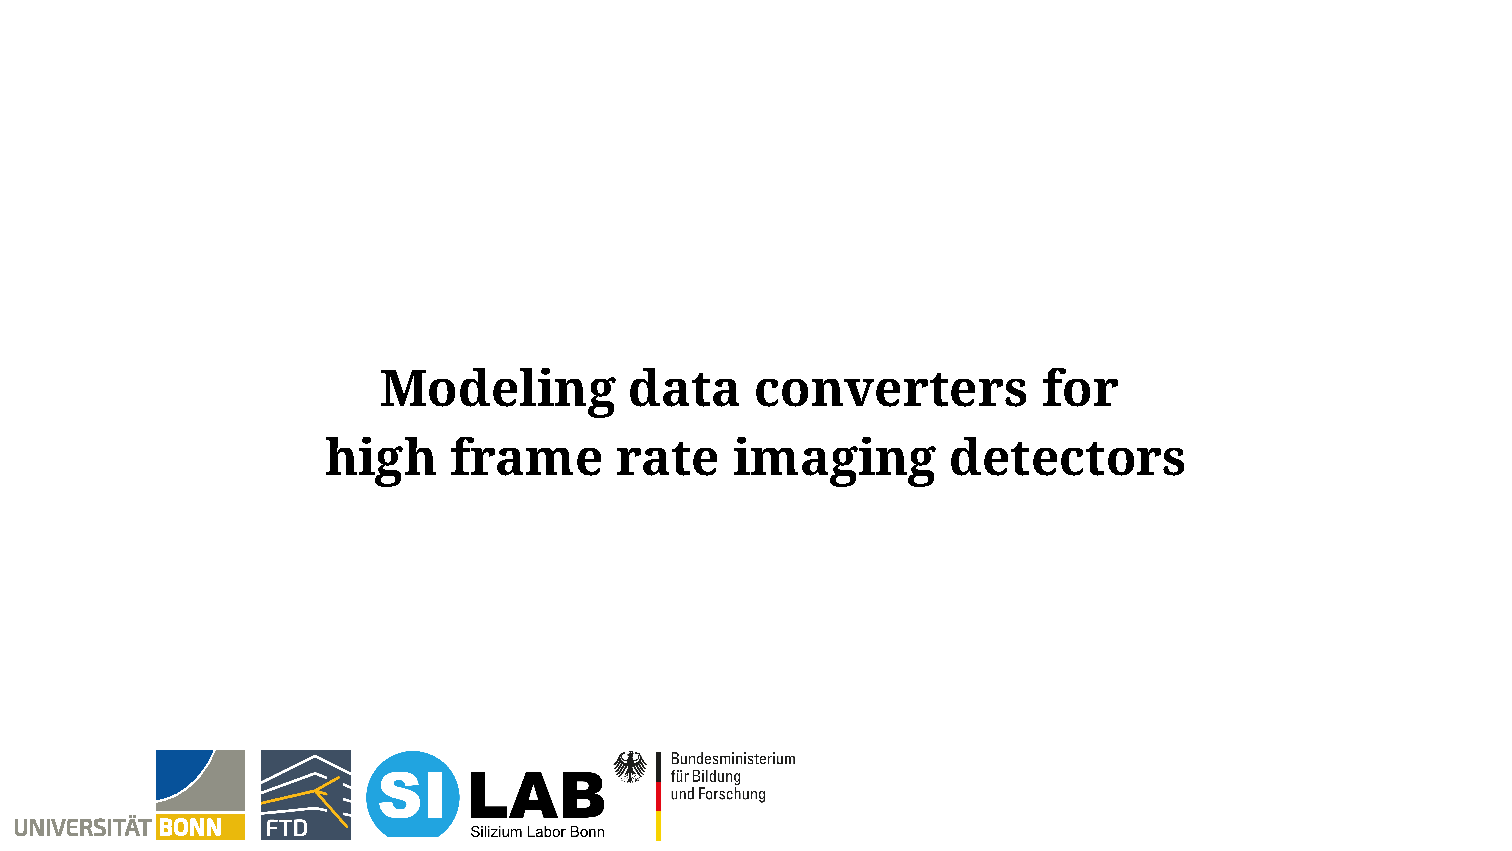
\includegraphics[width=\textwidth]{title.pdf}}

\frame{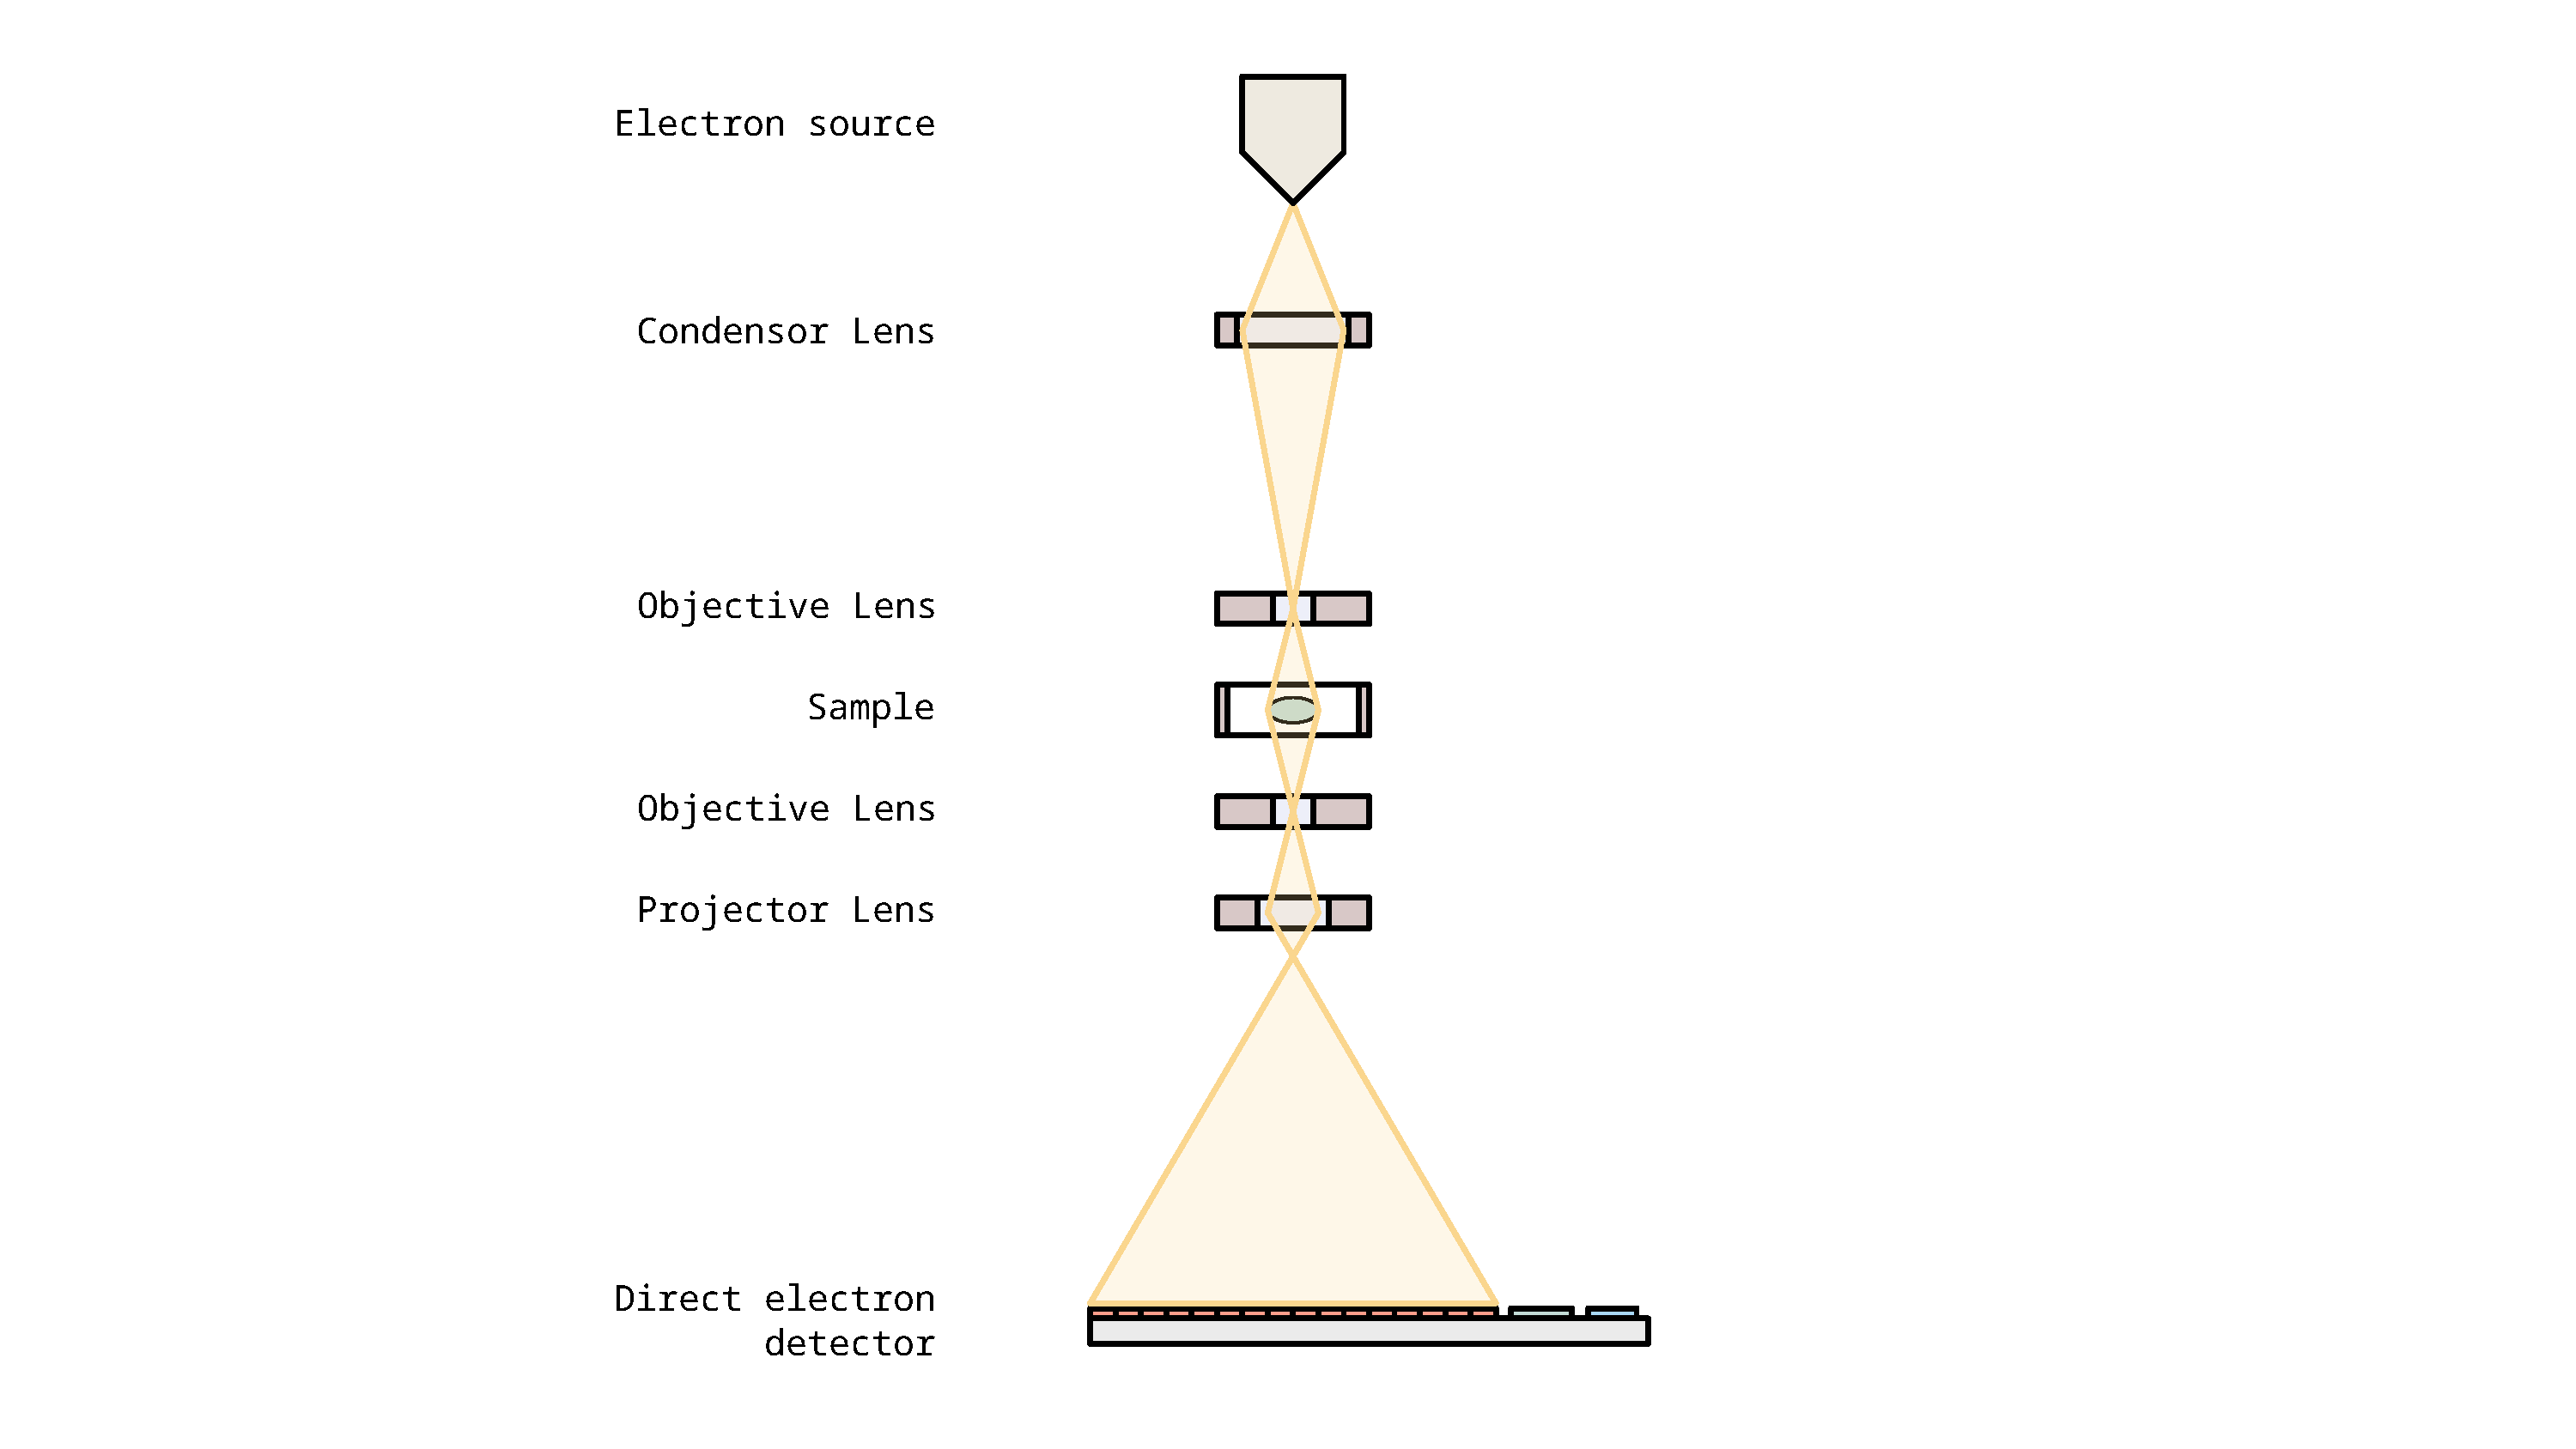
\includegraphics[width=\textwidth]{tem1.pdf}}
\frame{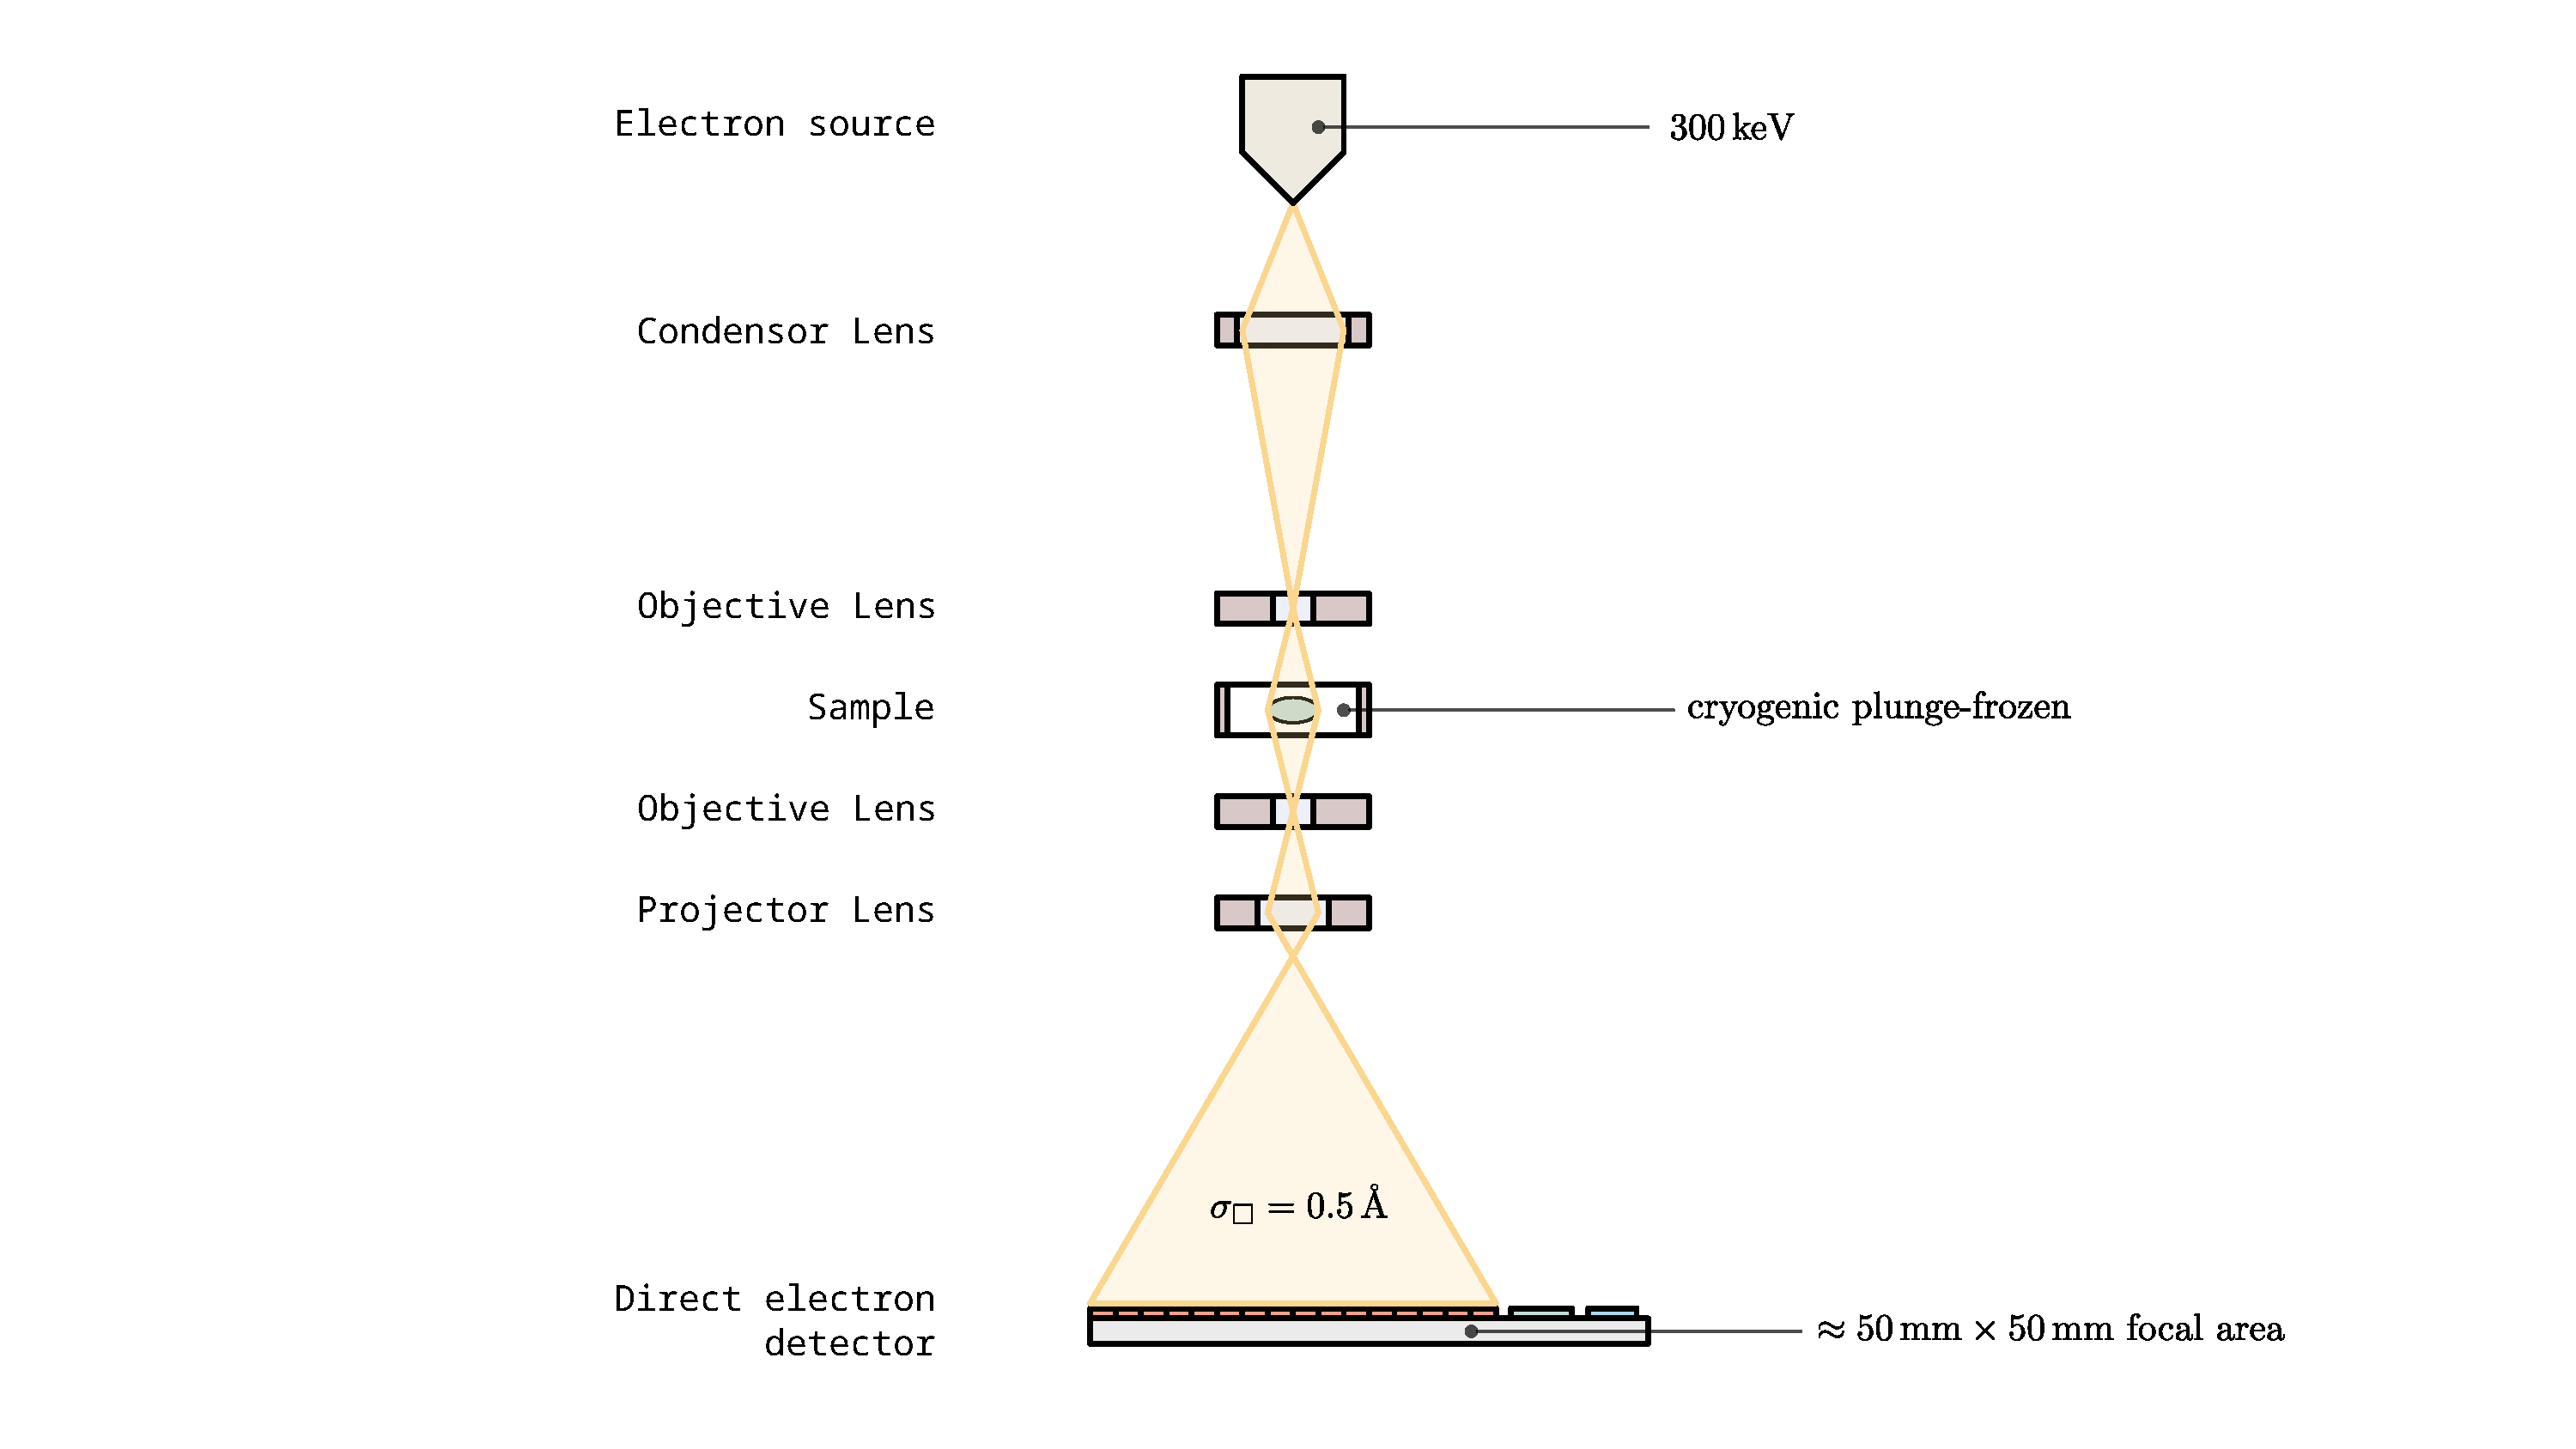
\includegraphics[width=\textwidth]{tem2.pdf}}
\frame{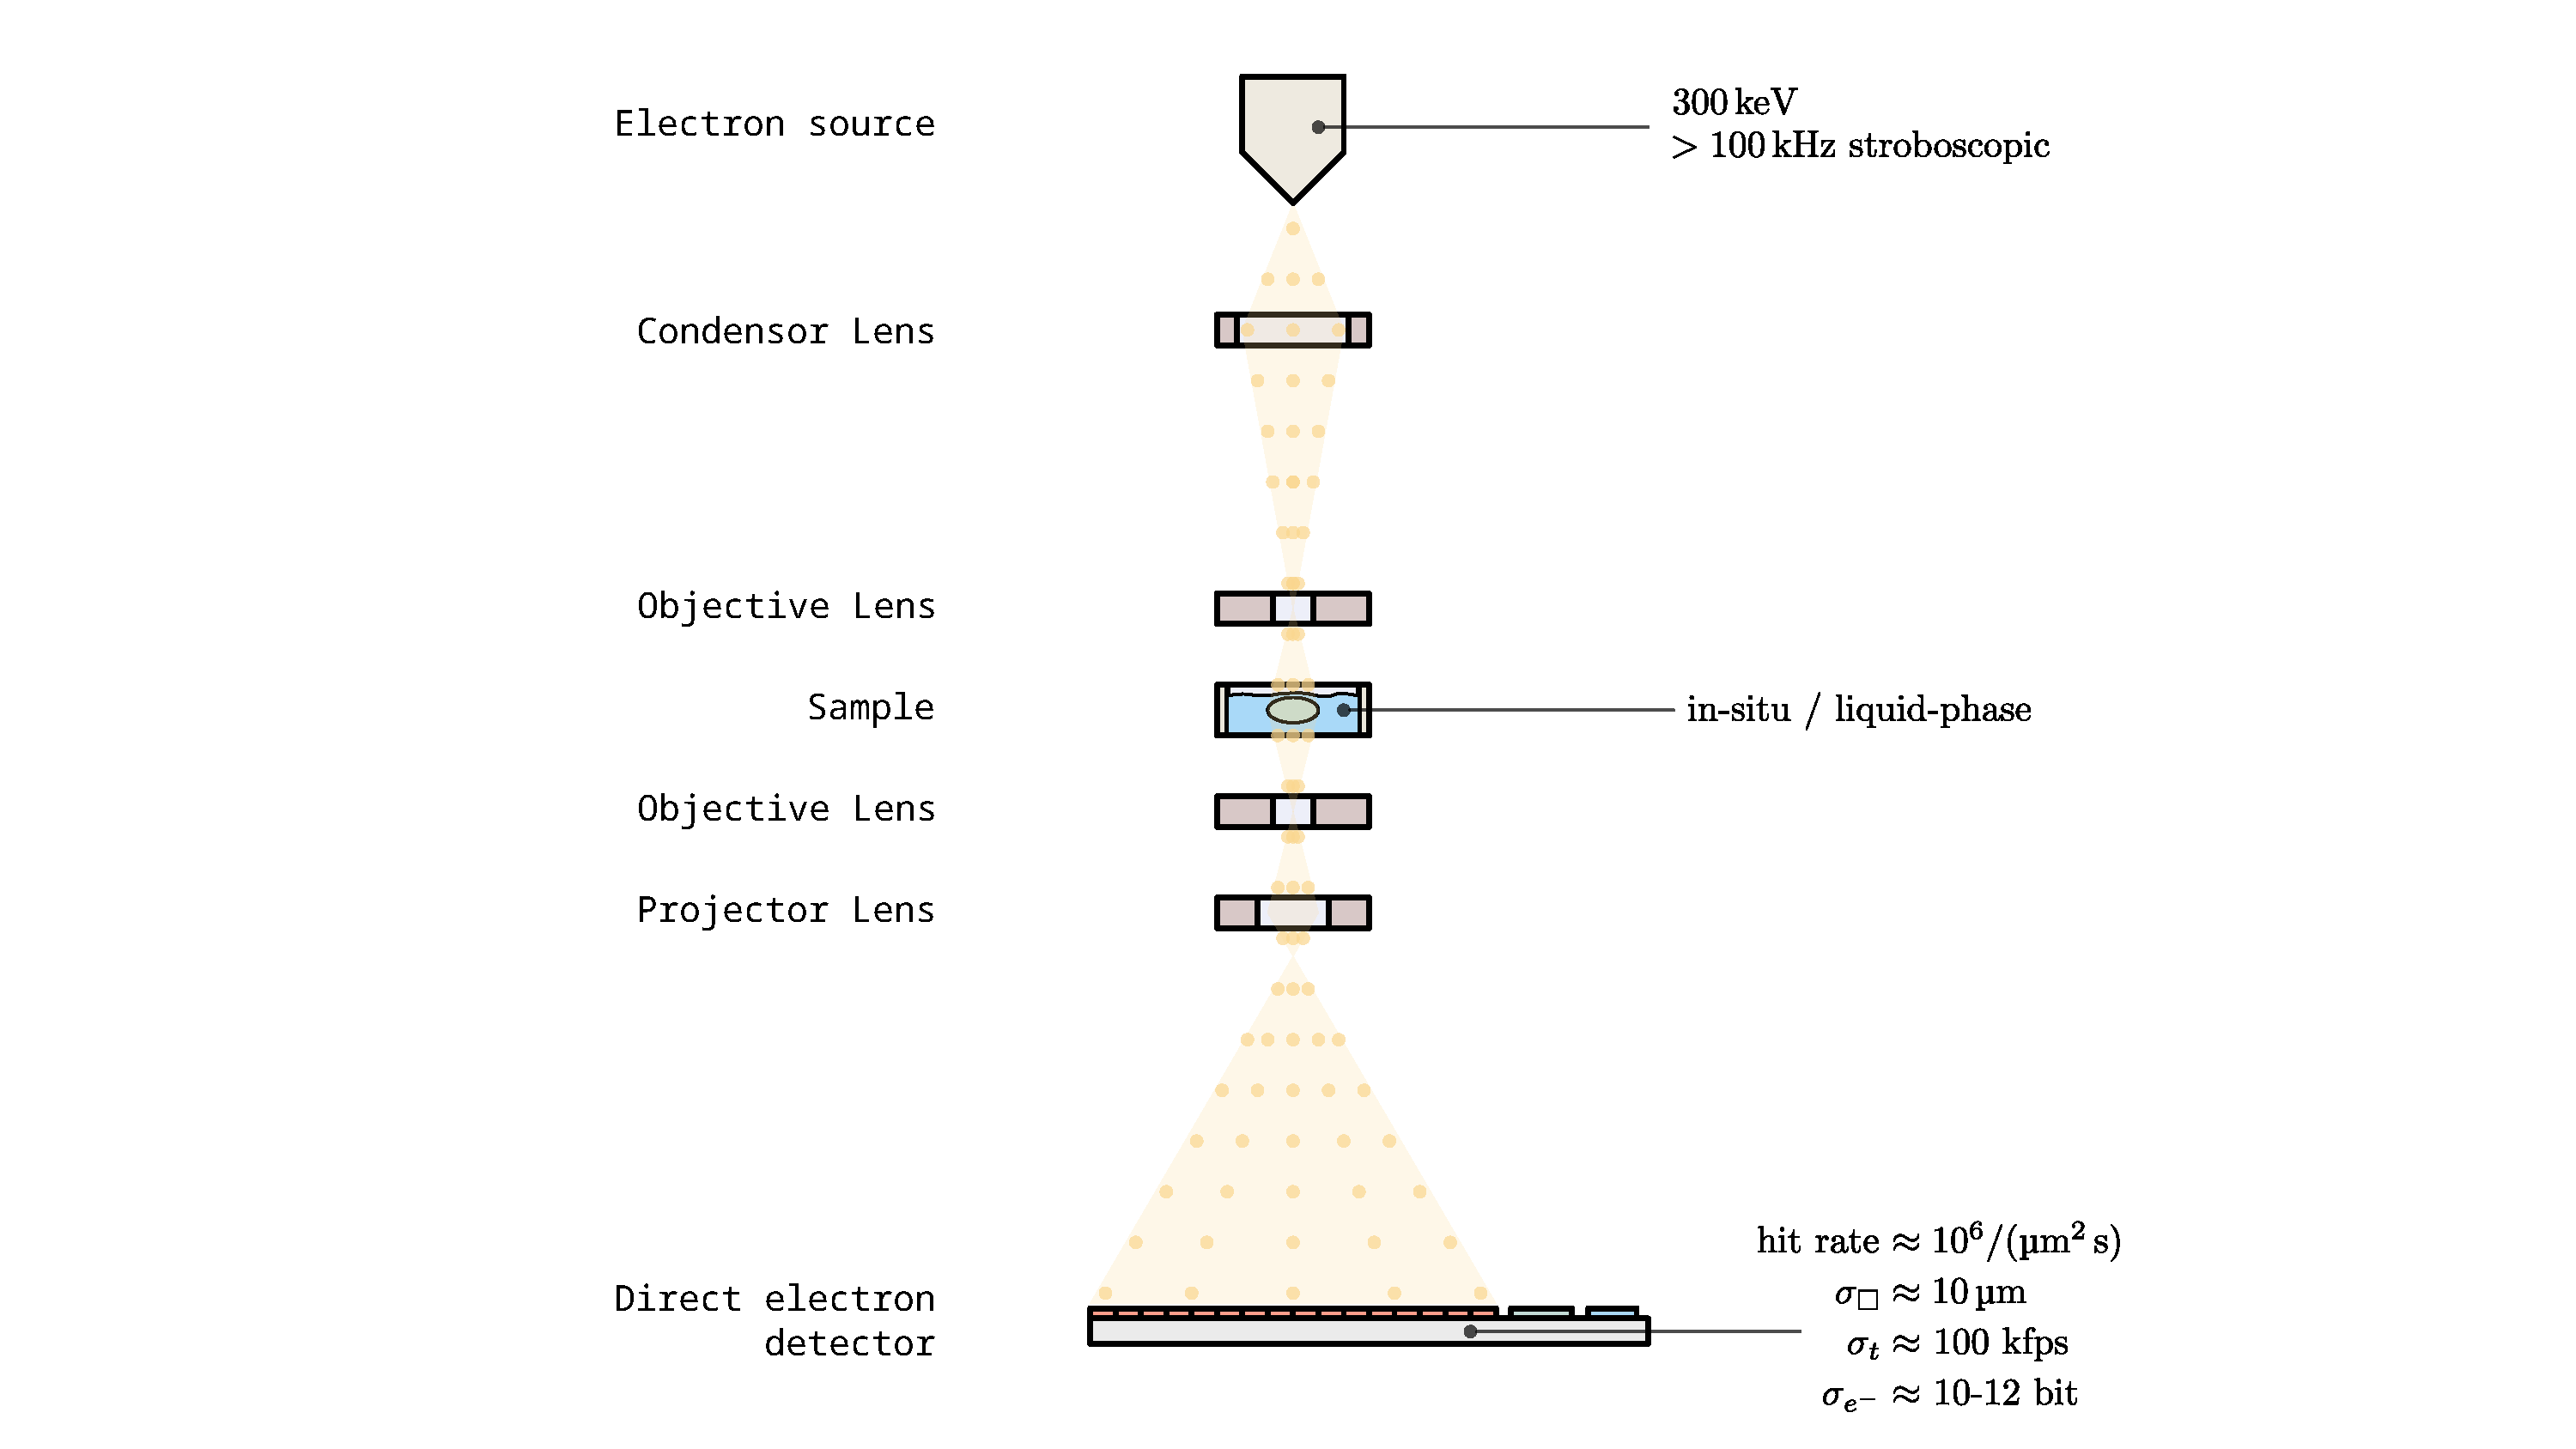
\includegraphics[width=\textwidth]{tem3.pdf}}
\frame{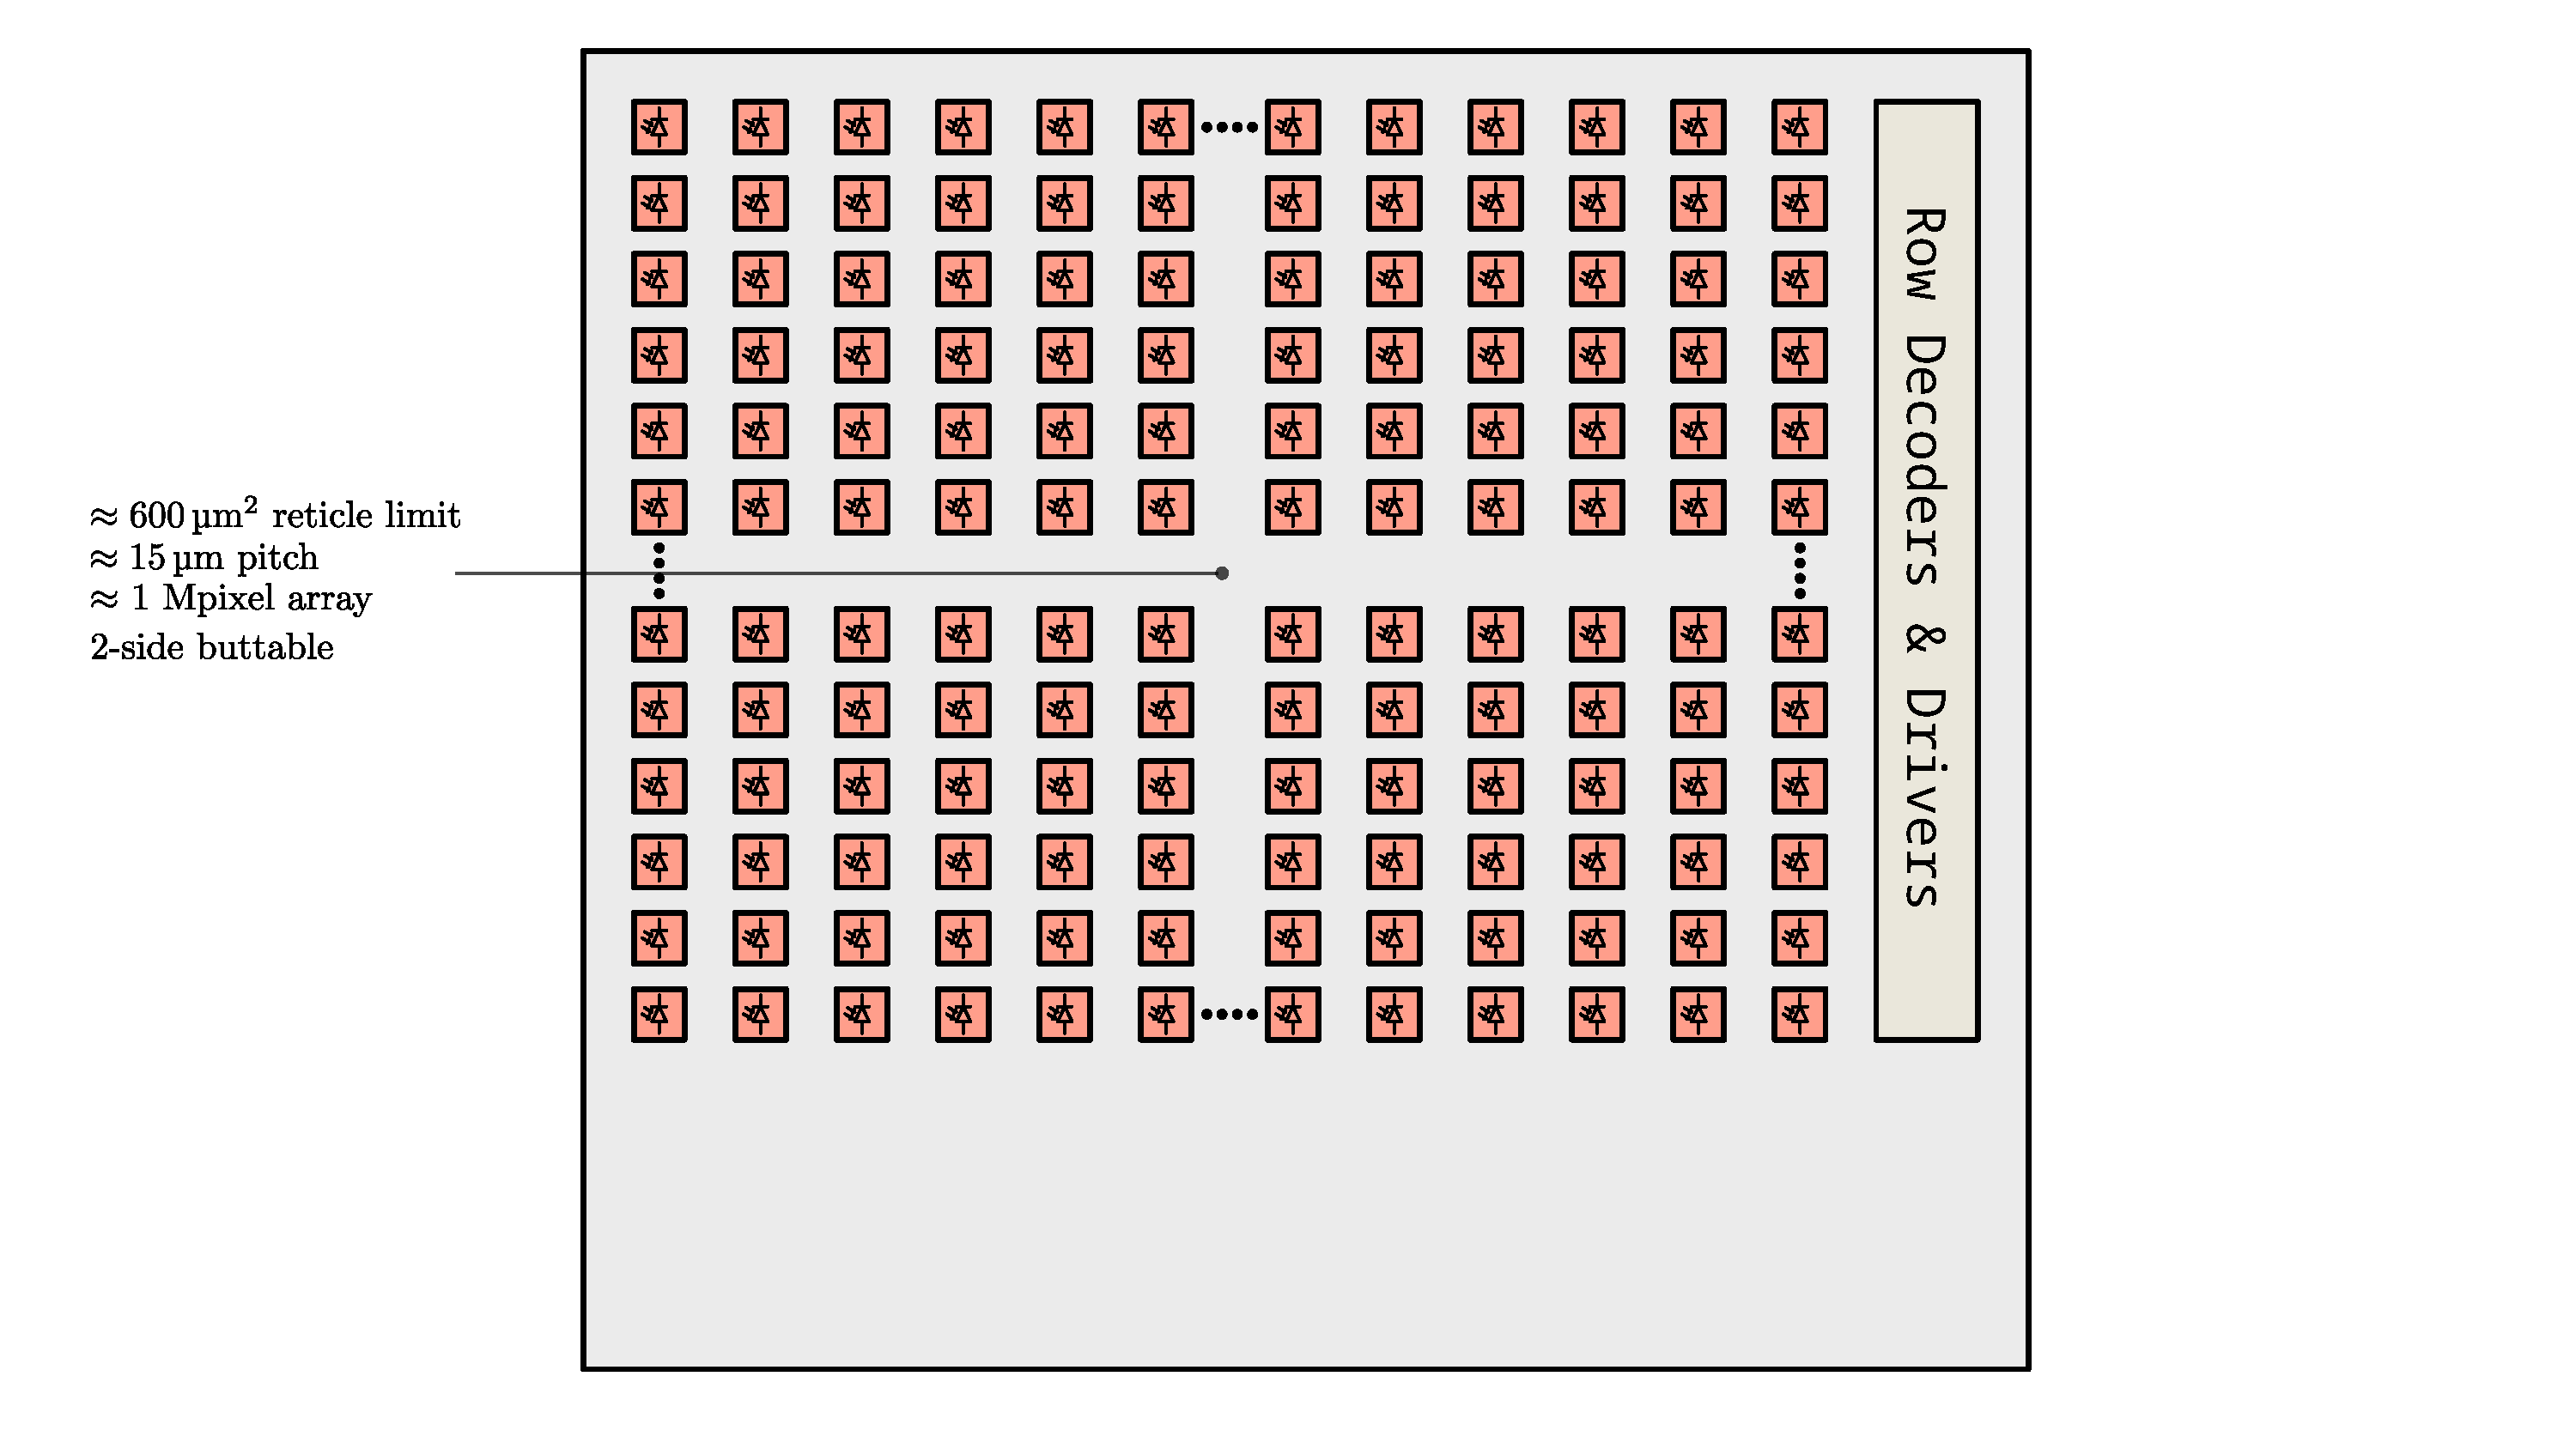
\includegraphics[width=\textwidth]{arch1.pdf}}
\frame{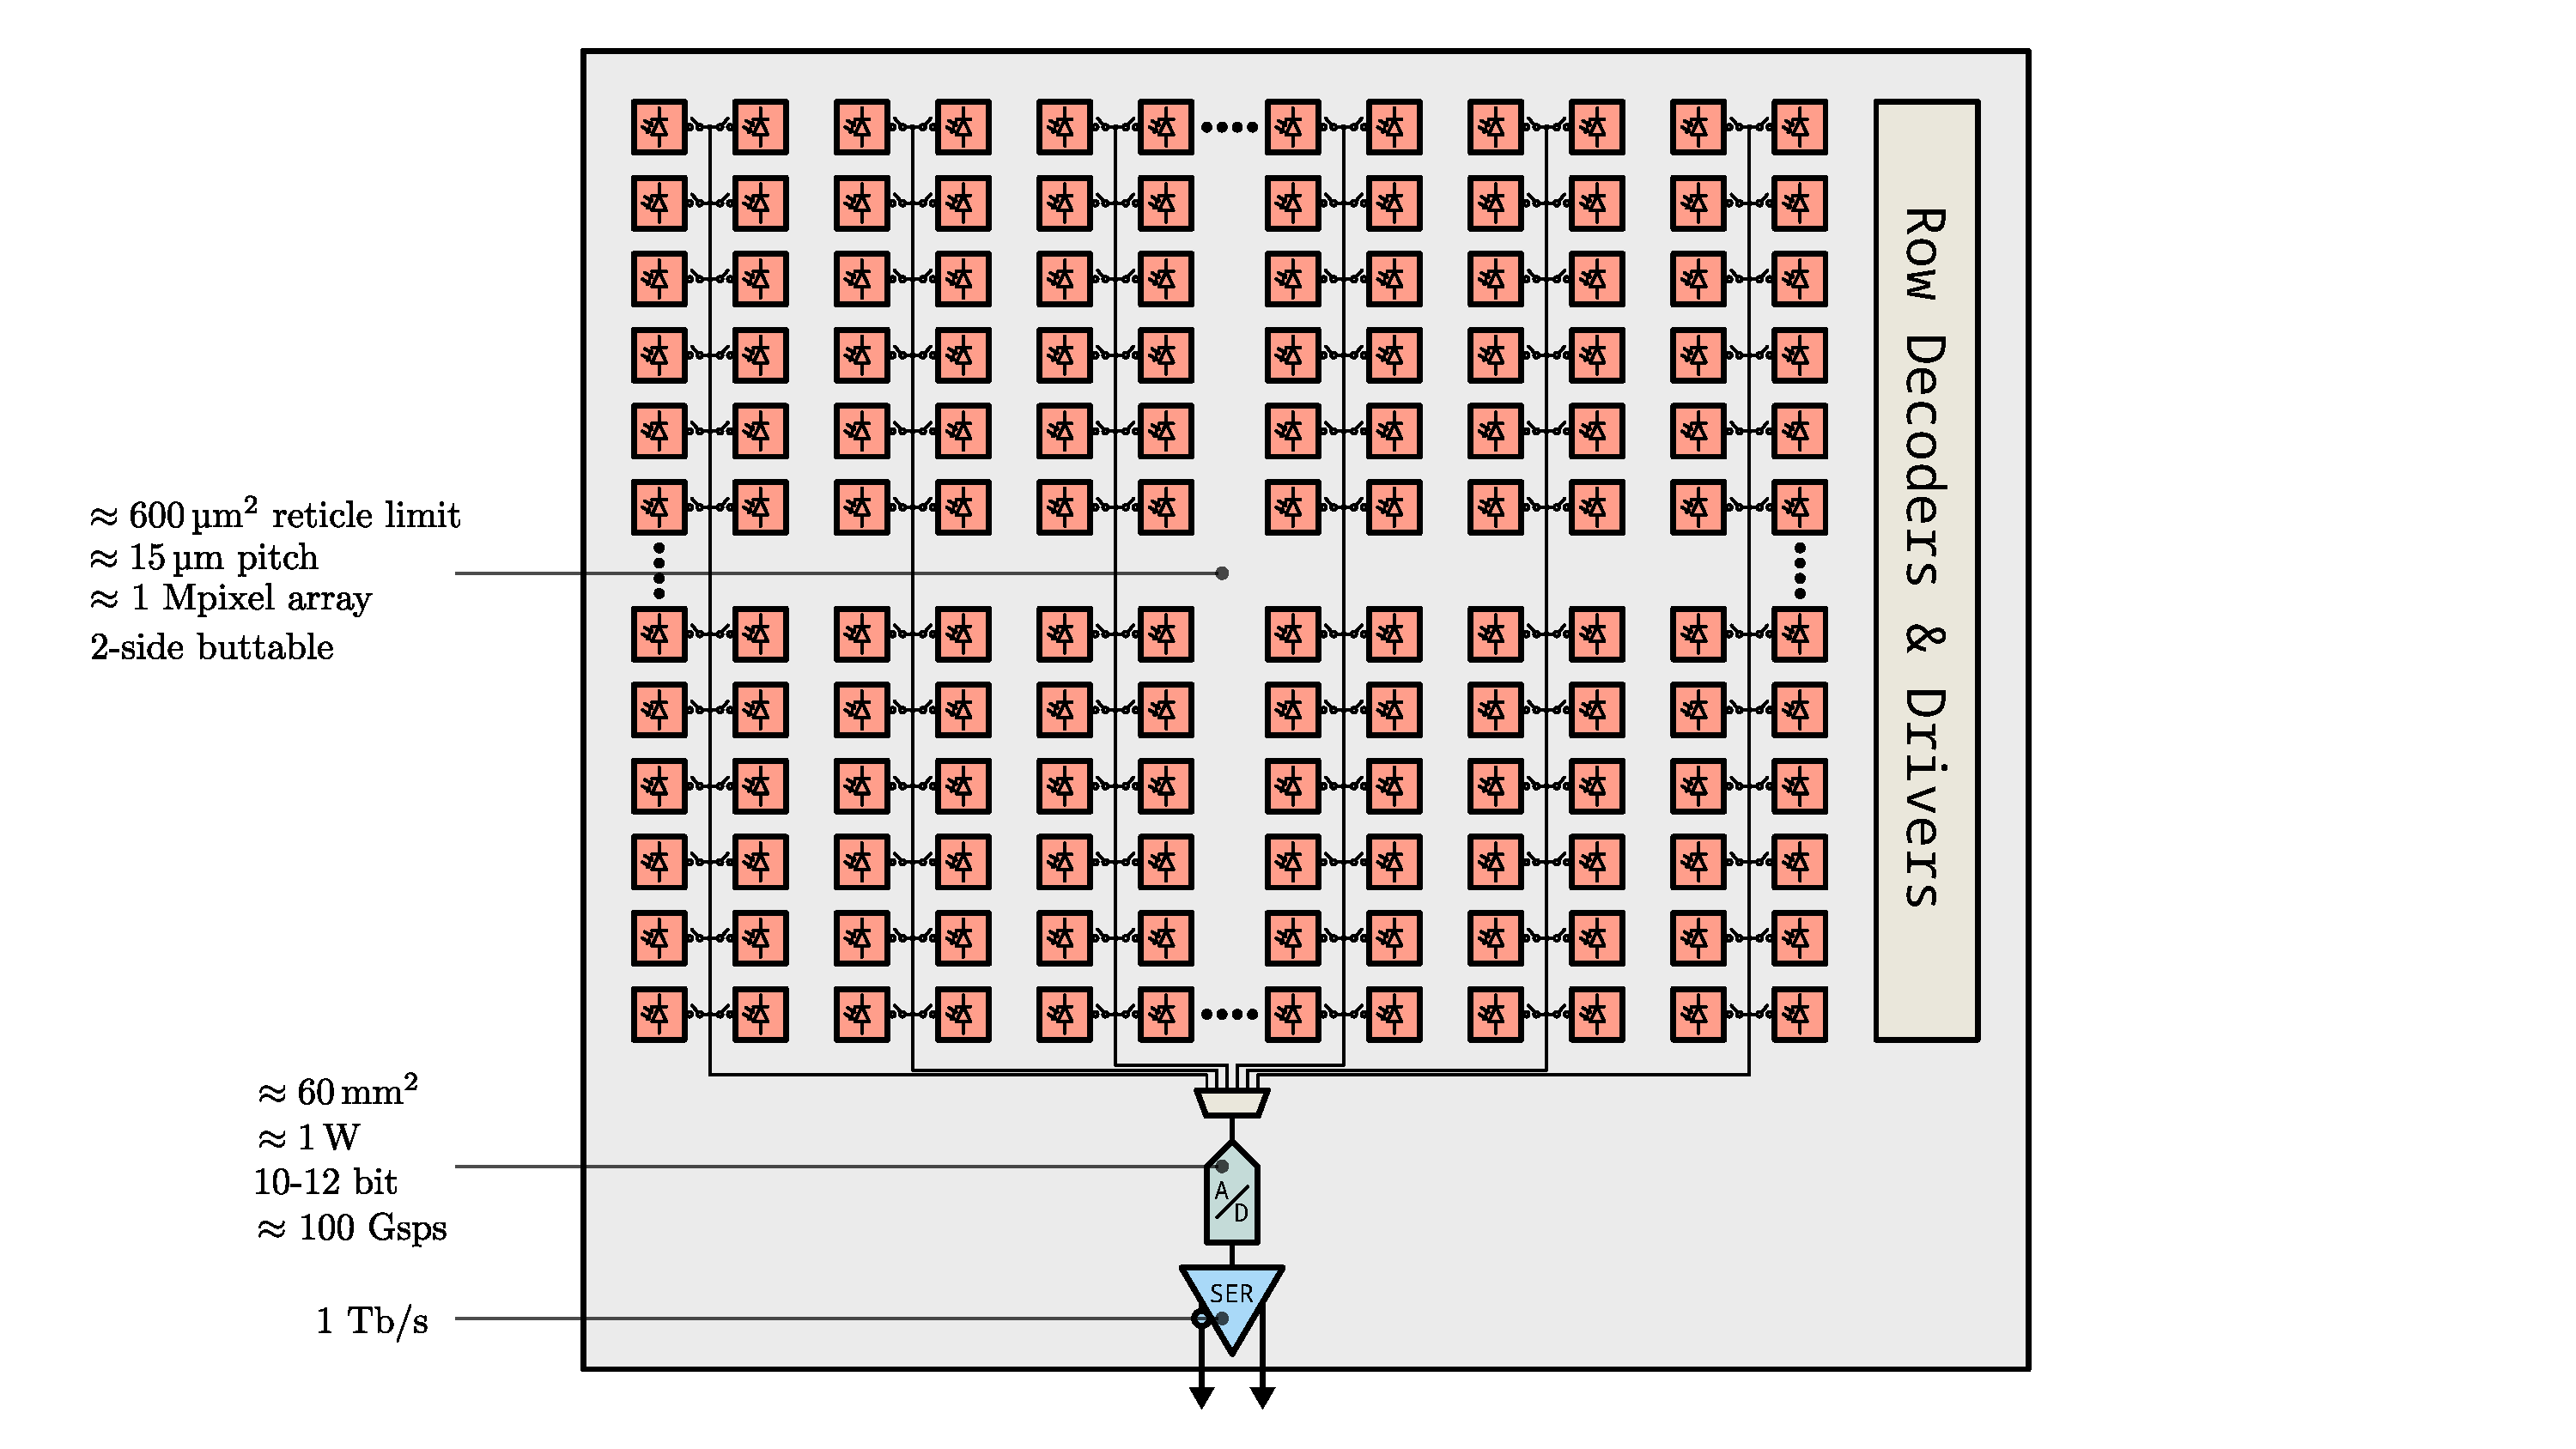
\includegraphics[width=\textwidth]{arch2.pdf}}
\frame{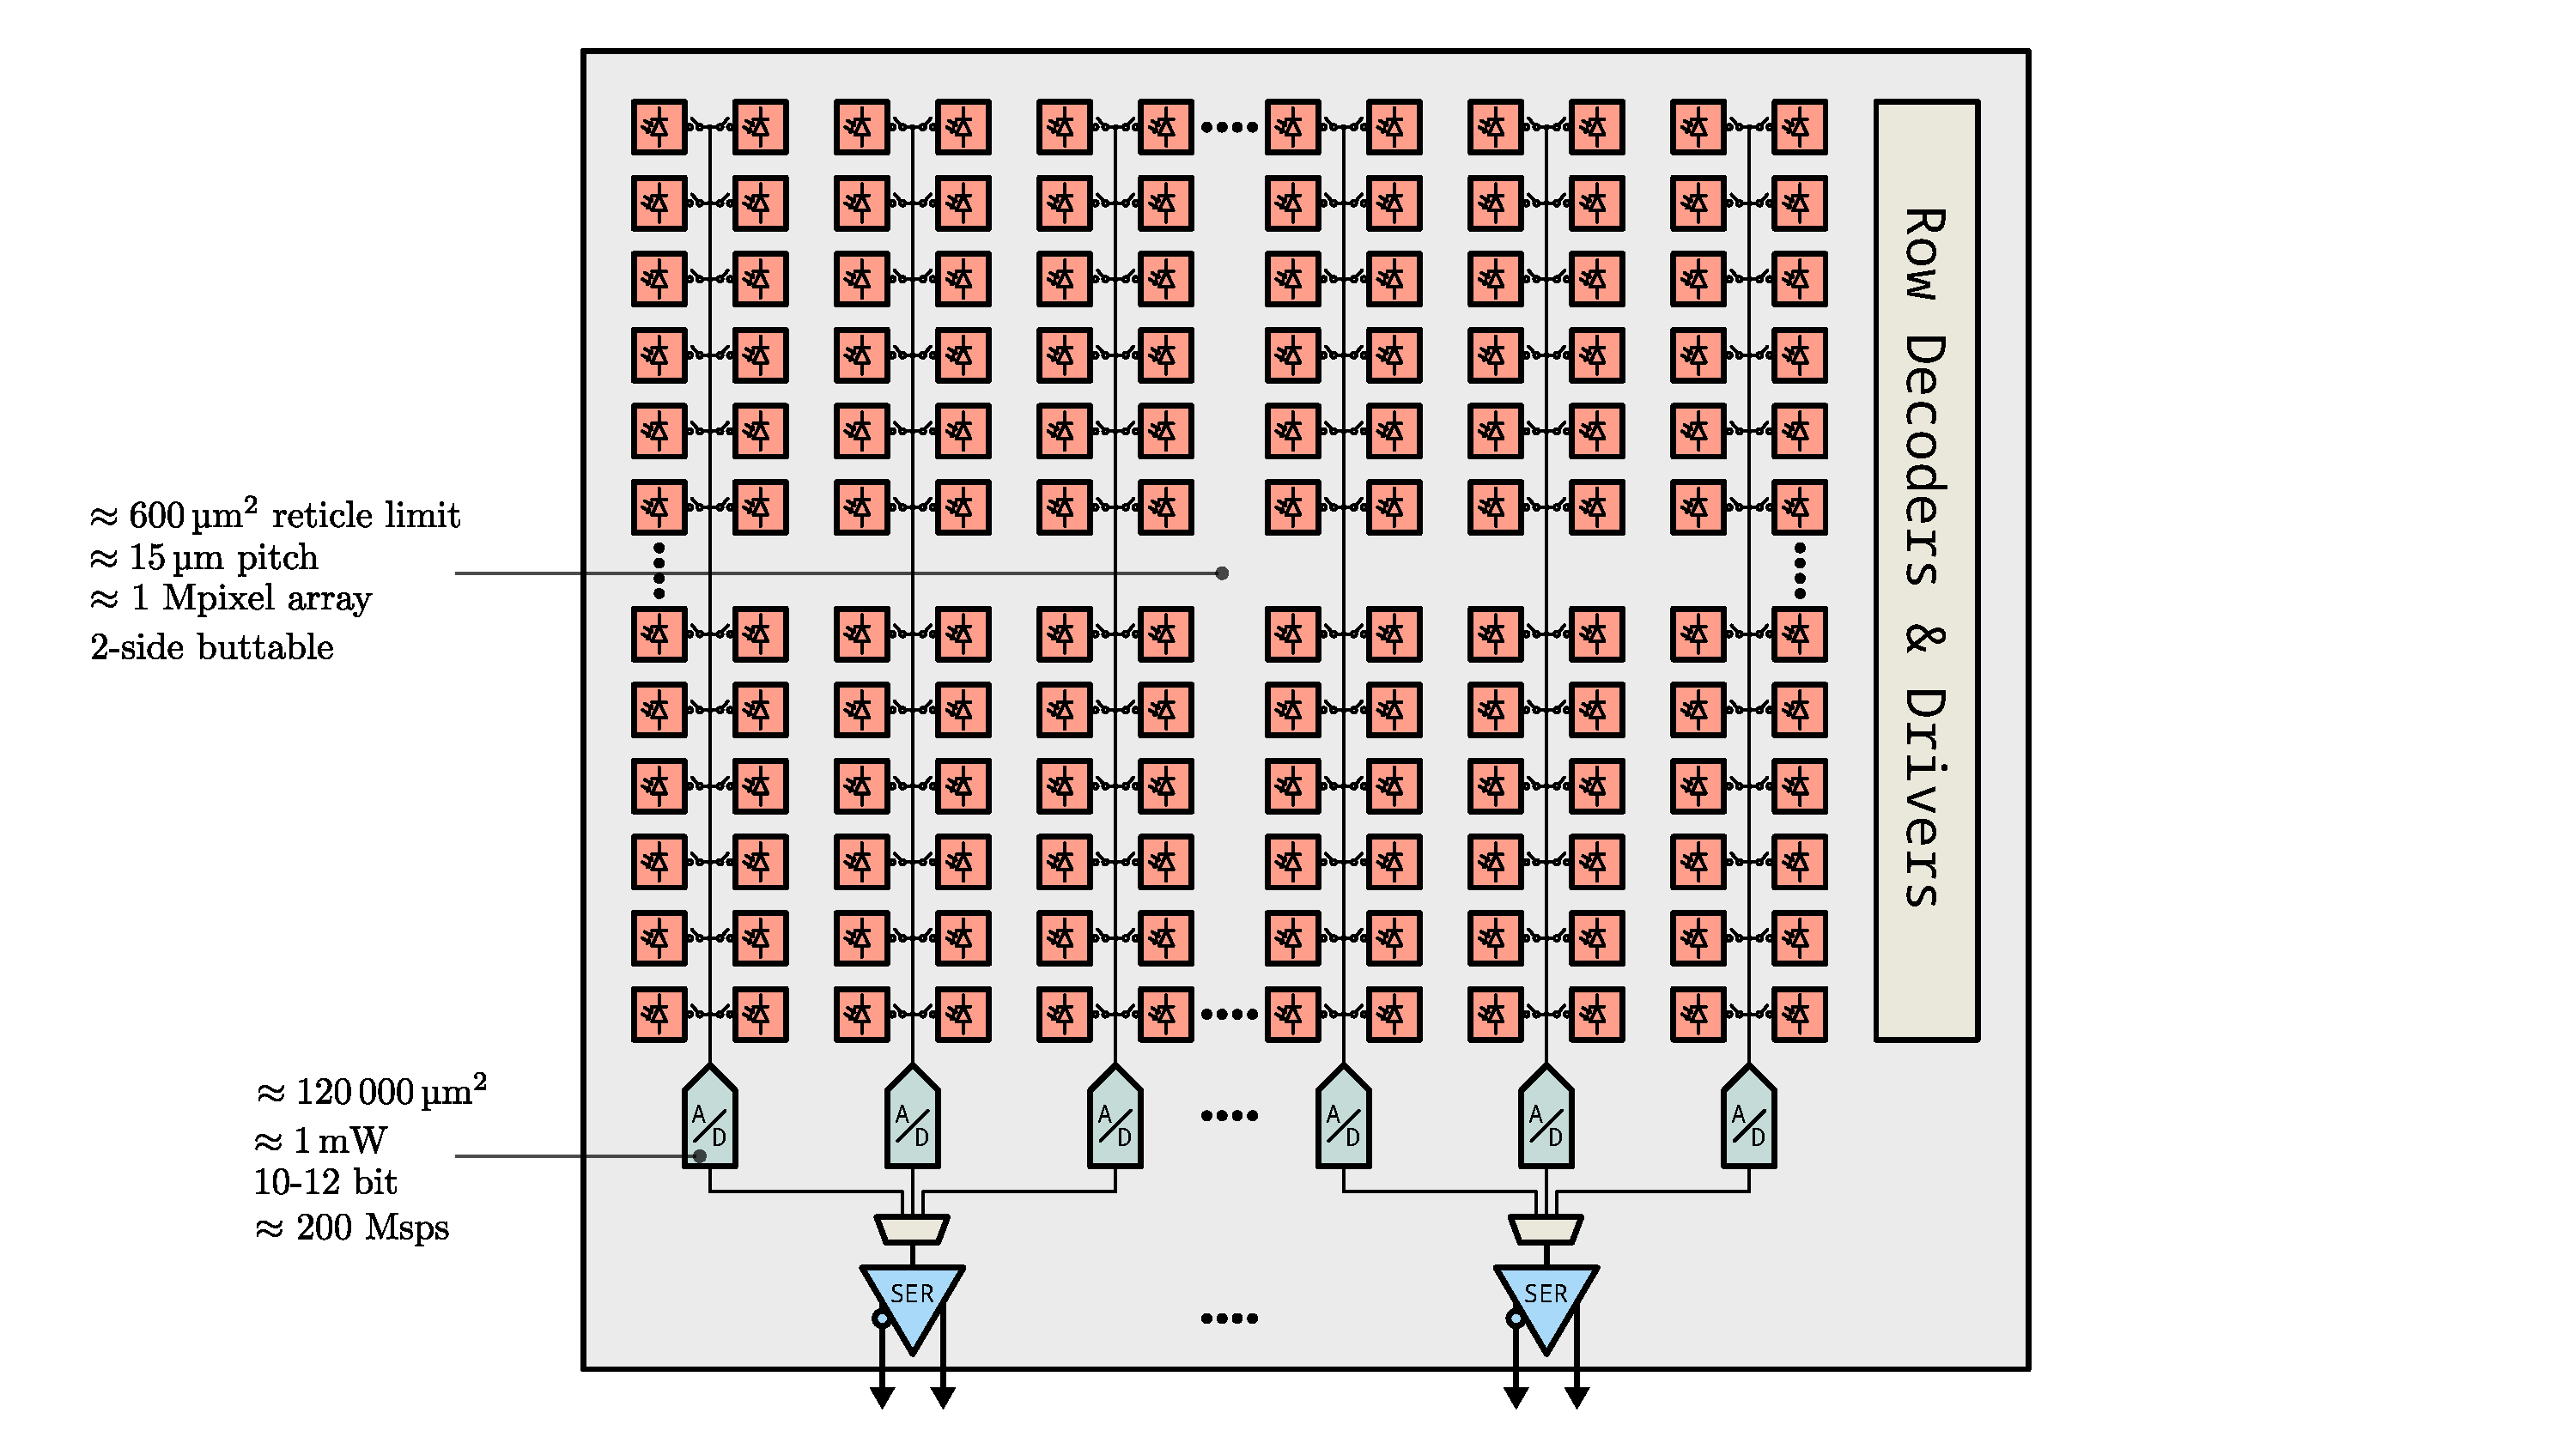
\includegraphics[width=\textwidth]{arch3.pdf}}
\frame{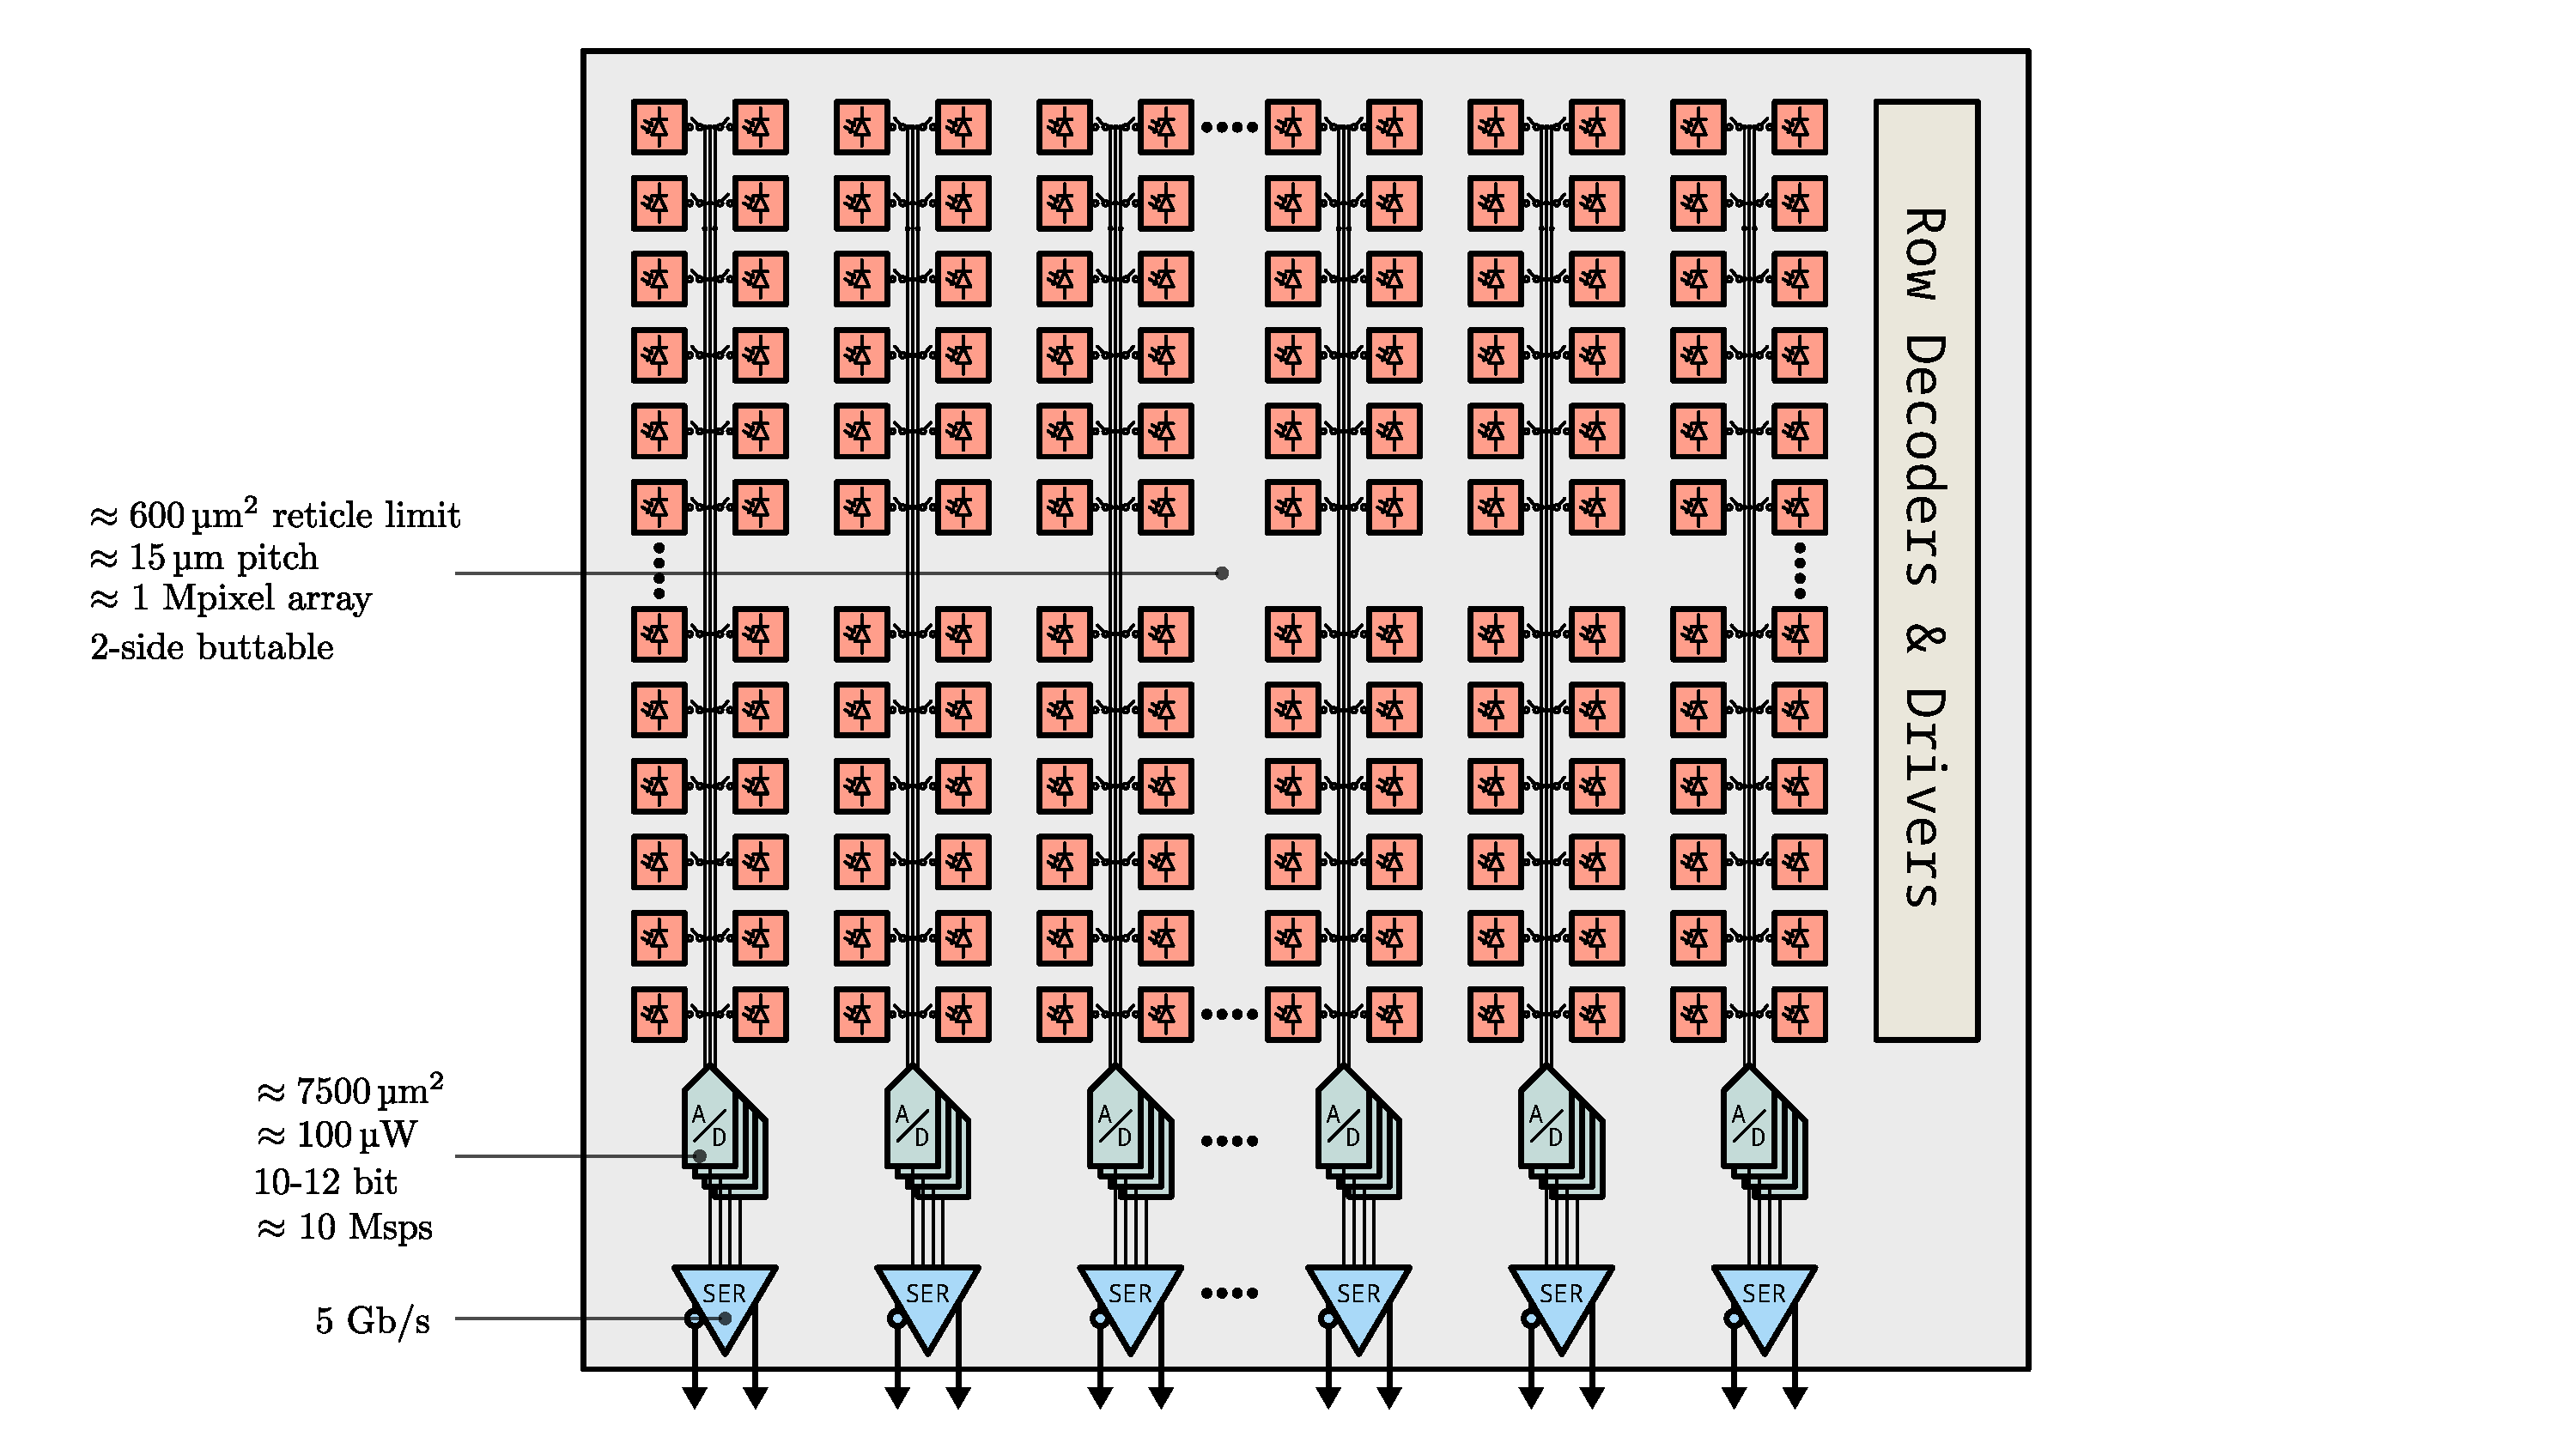
\includegraphics[width=\textwidth]{arch4.pdf}}
\frame{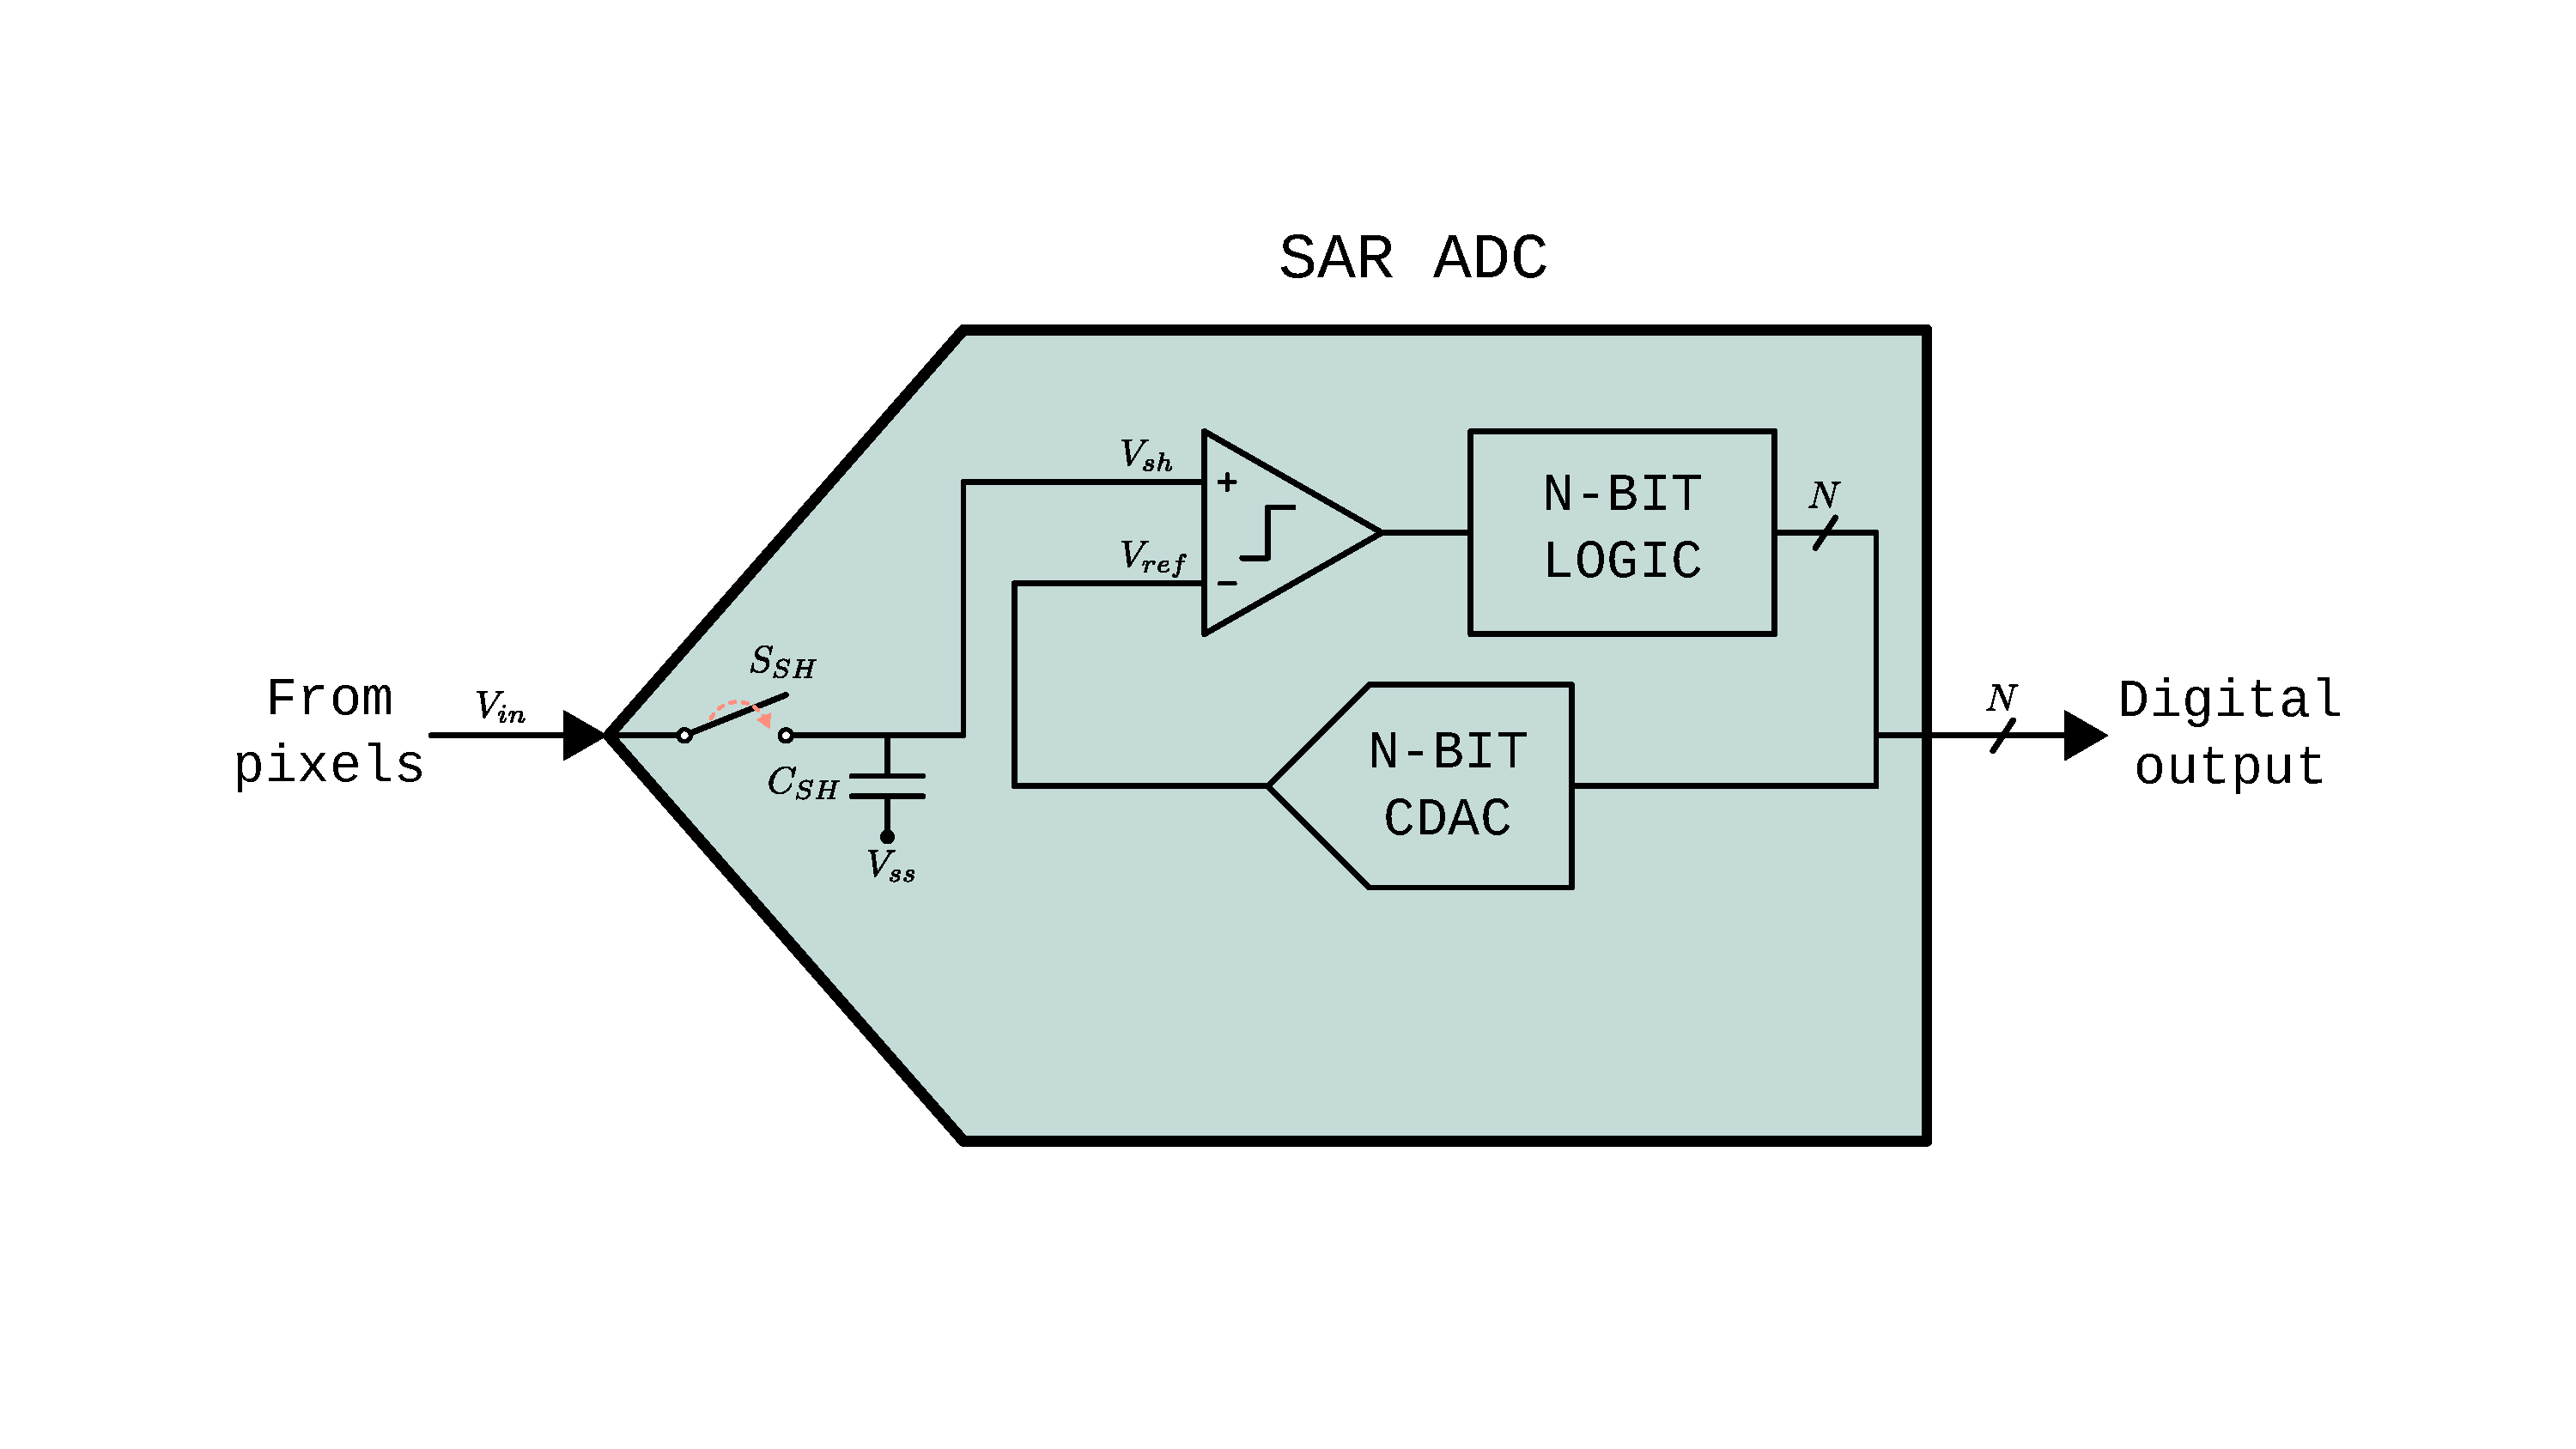
\includegraphics[width=\textwidth]{adc1.pdf}}
\frame{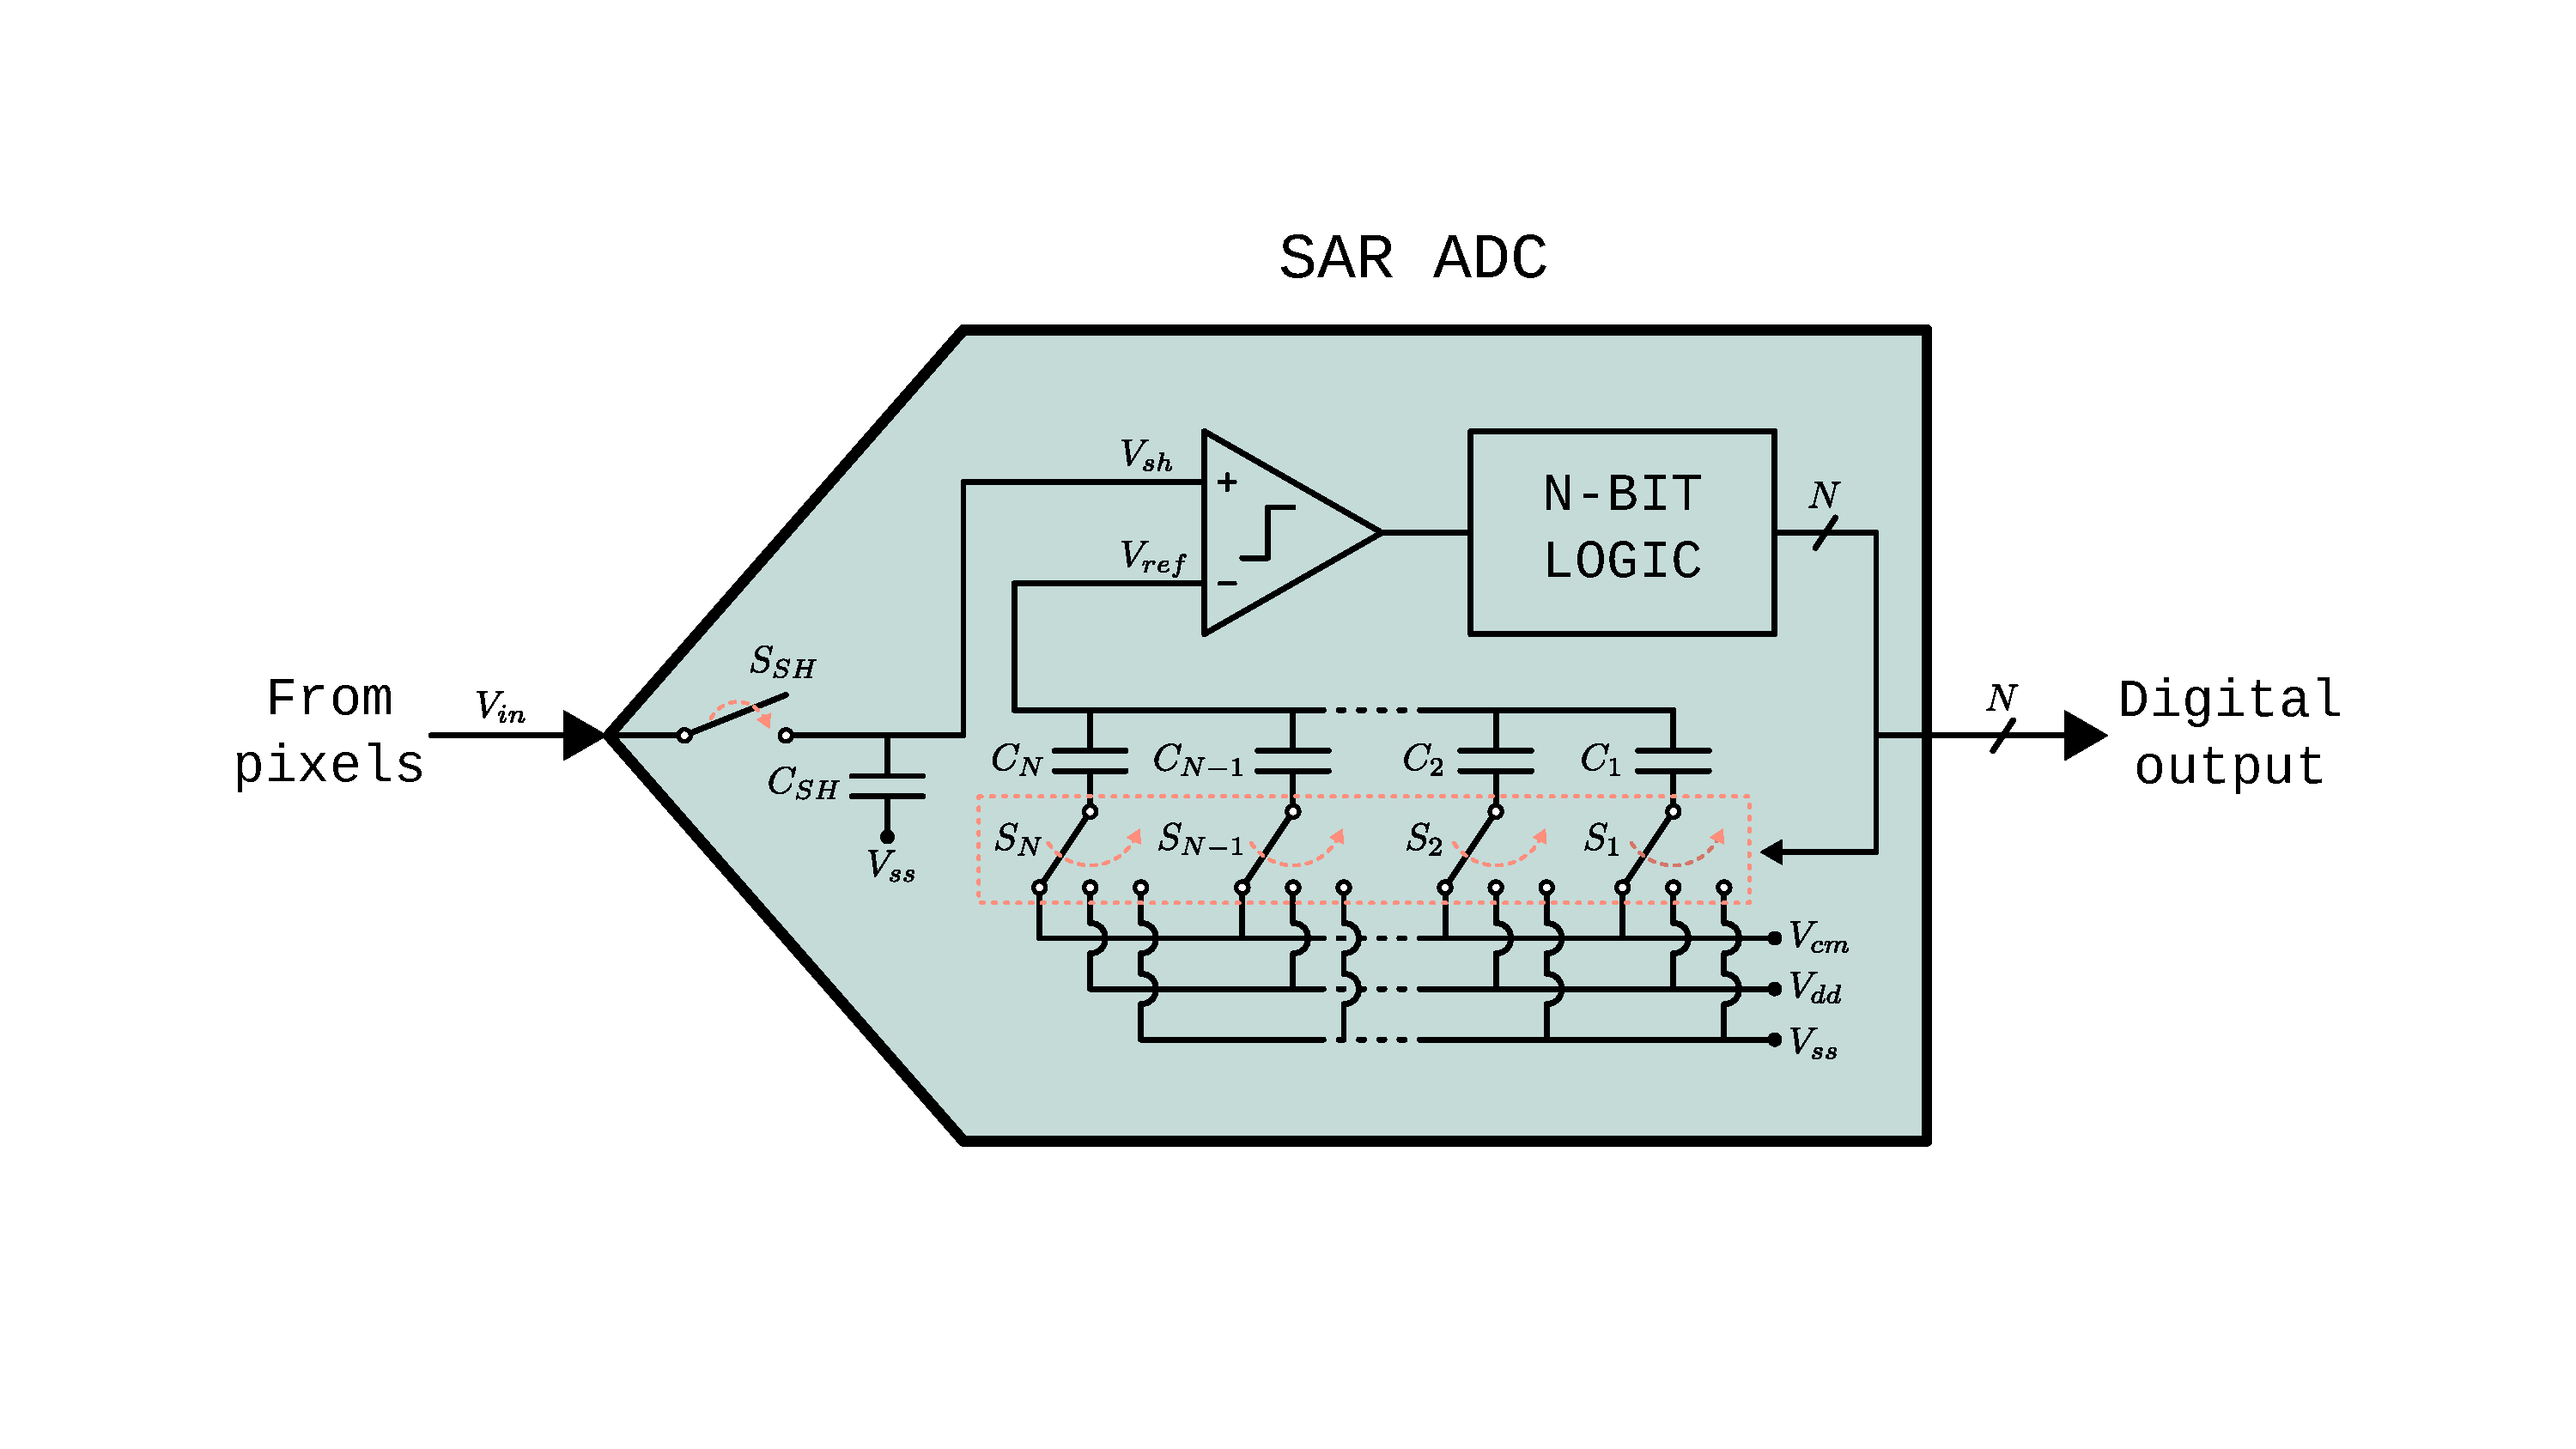
\includegraphics[width=\textwidth]{adc2.pdf}}

\frame{
  \frametitle{Basic ideal operation}
  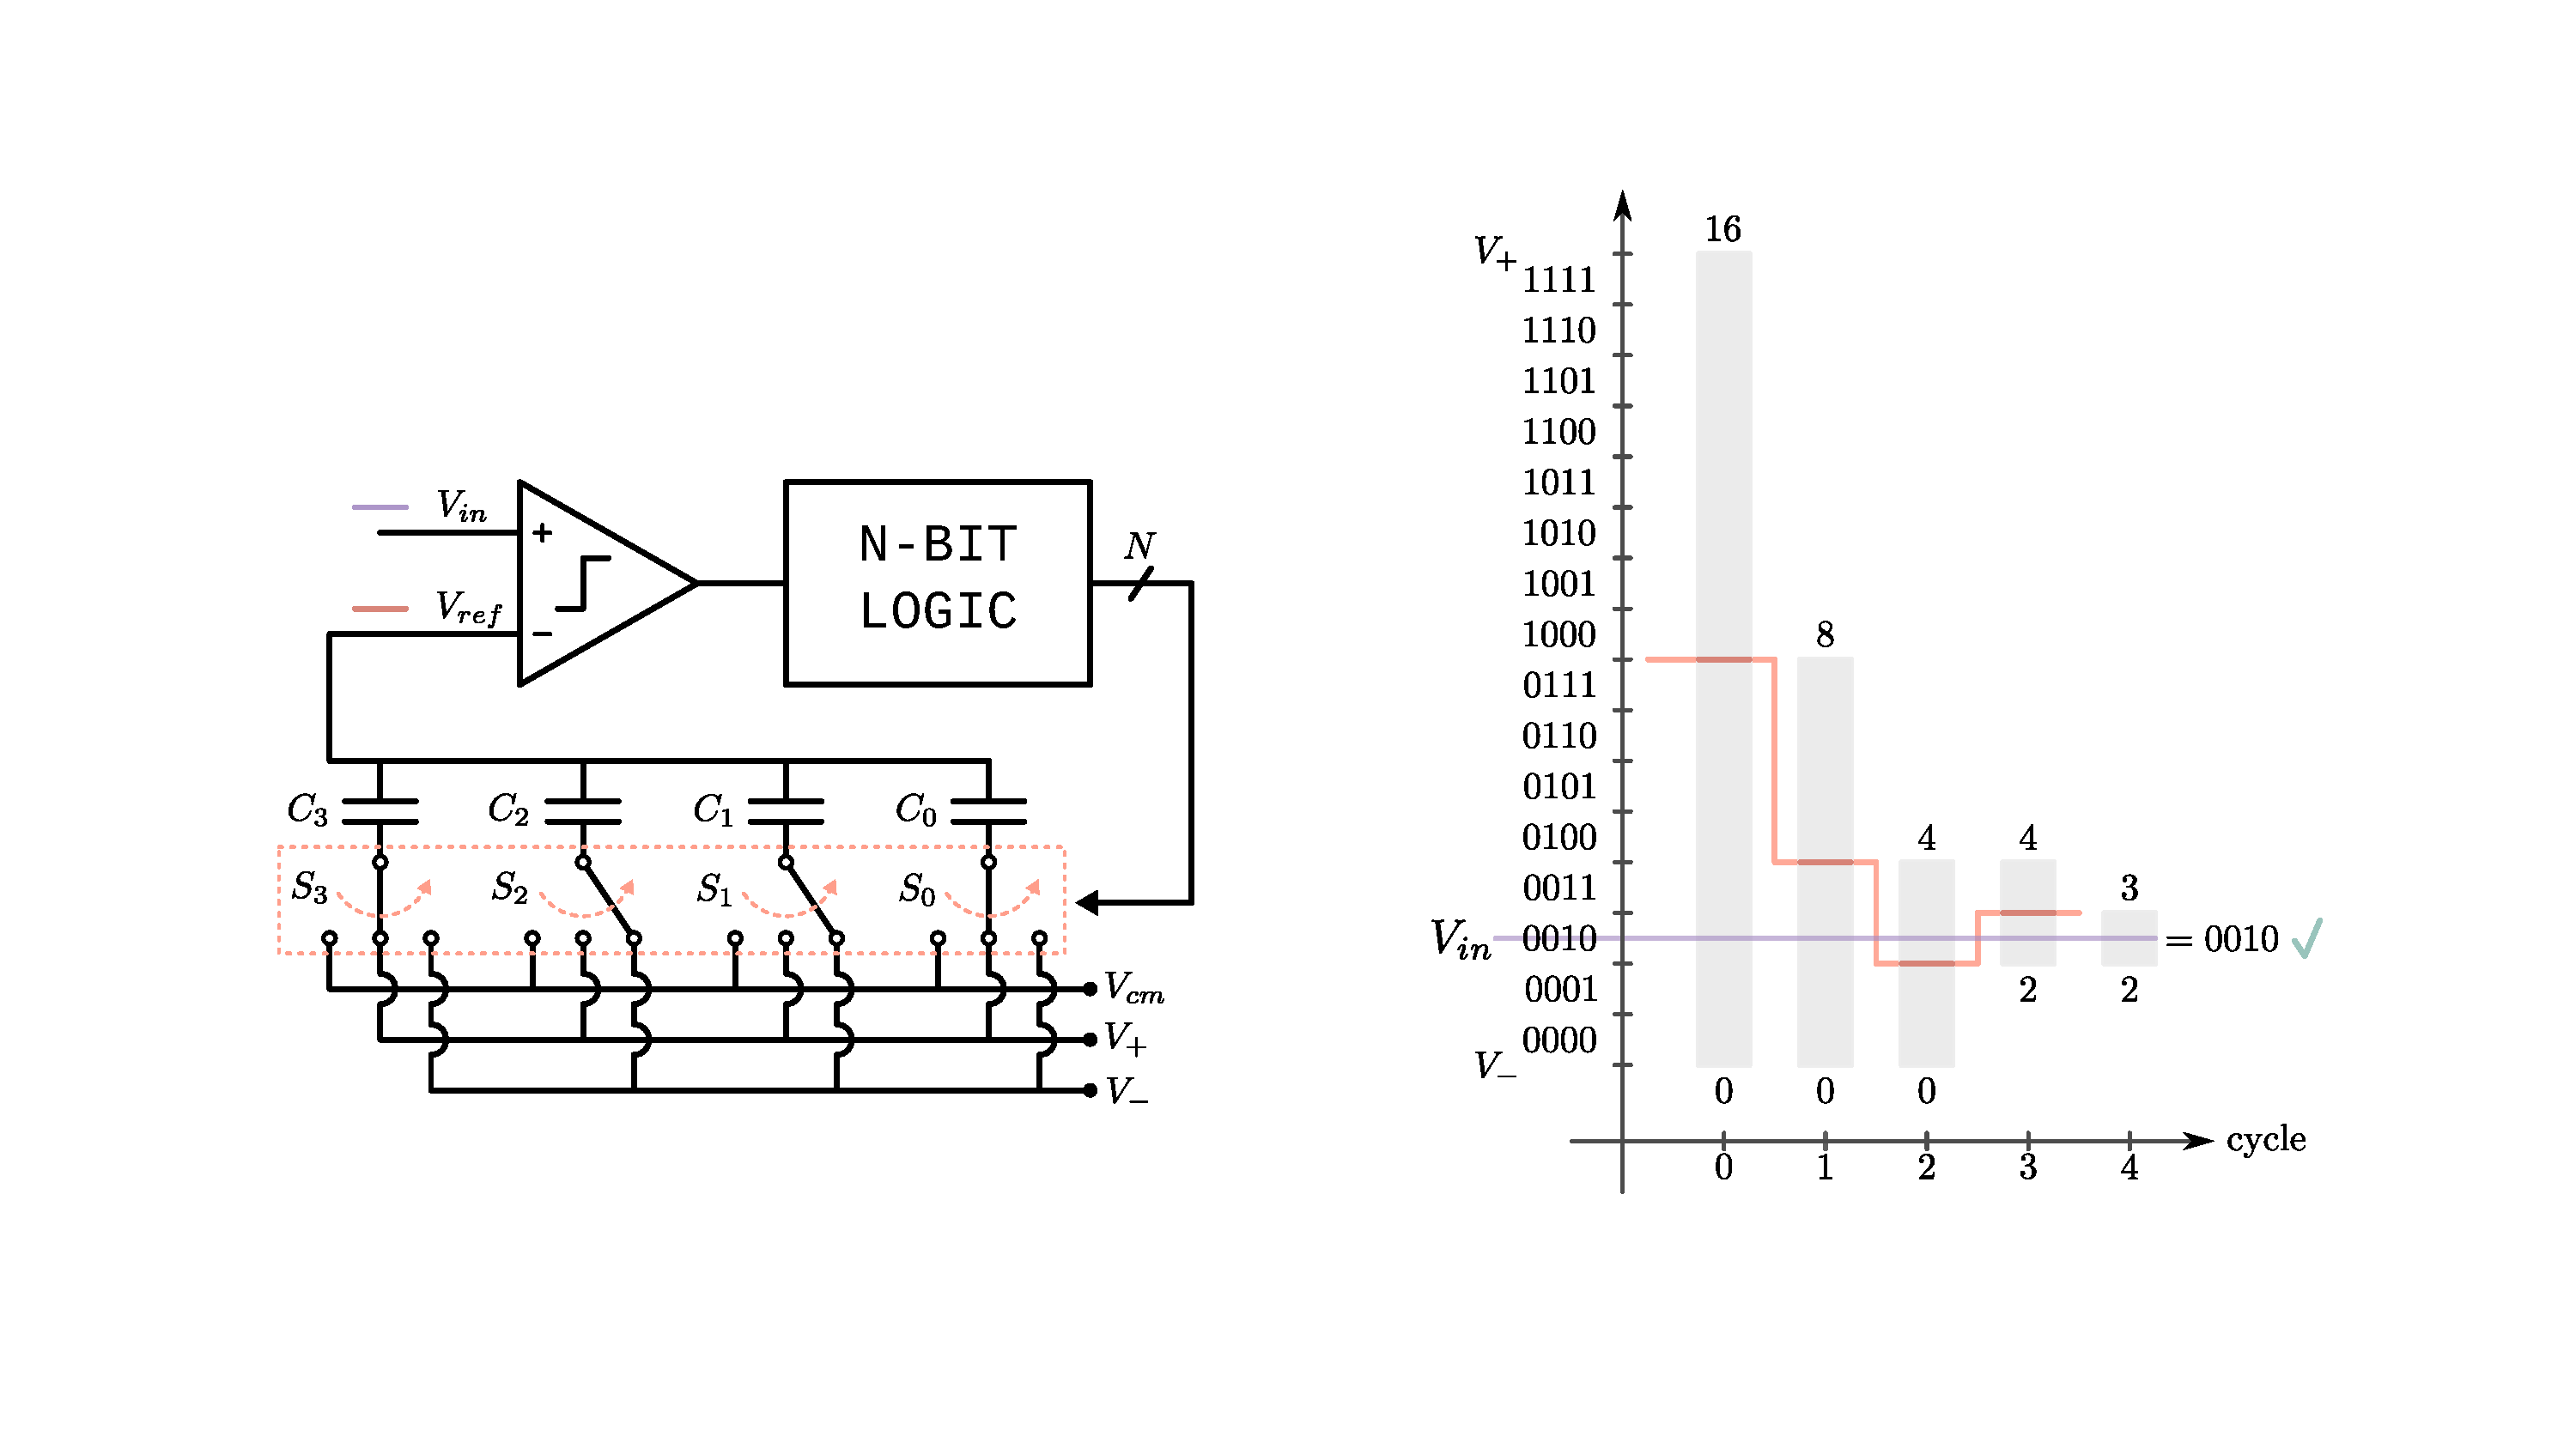
\includegraphics[width=\textwidth]{tranchar1.pdf}
  }
\frame{\frametitle{Threshold and reference noise (dynamic error)}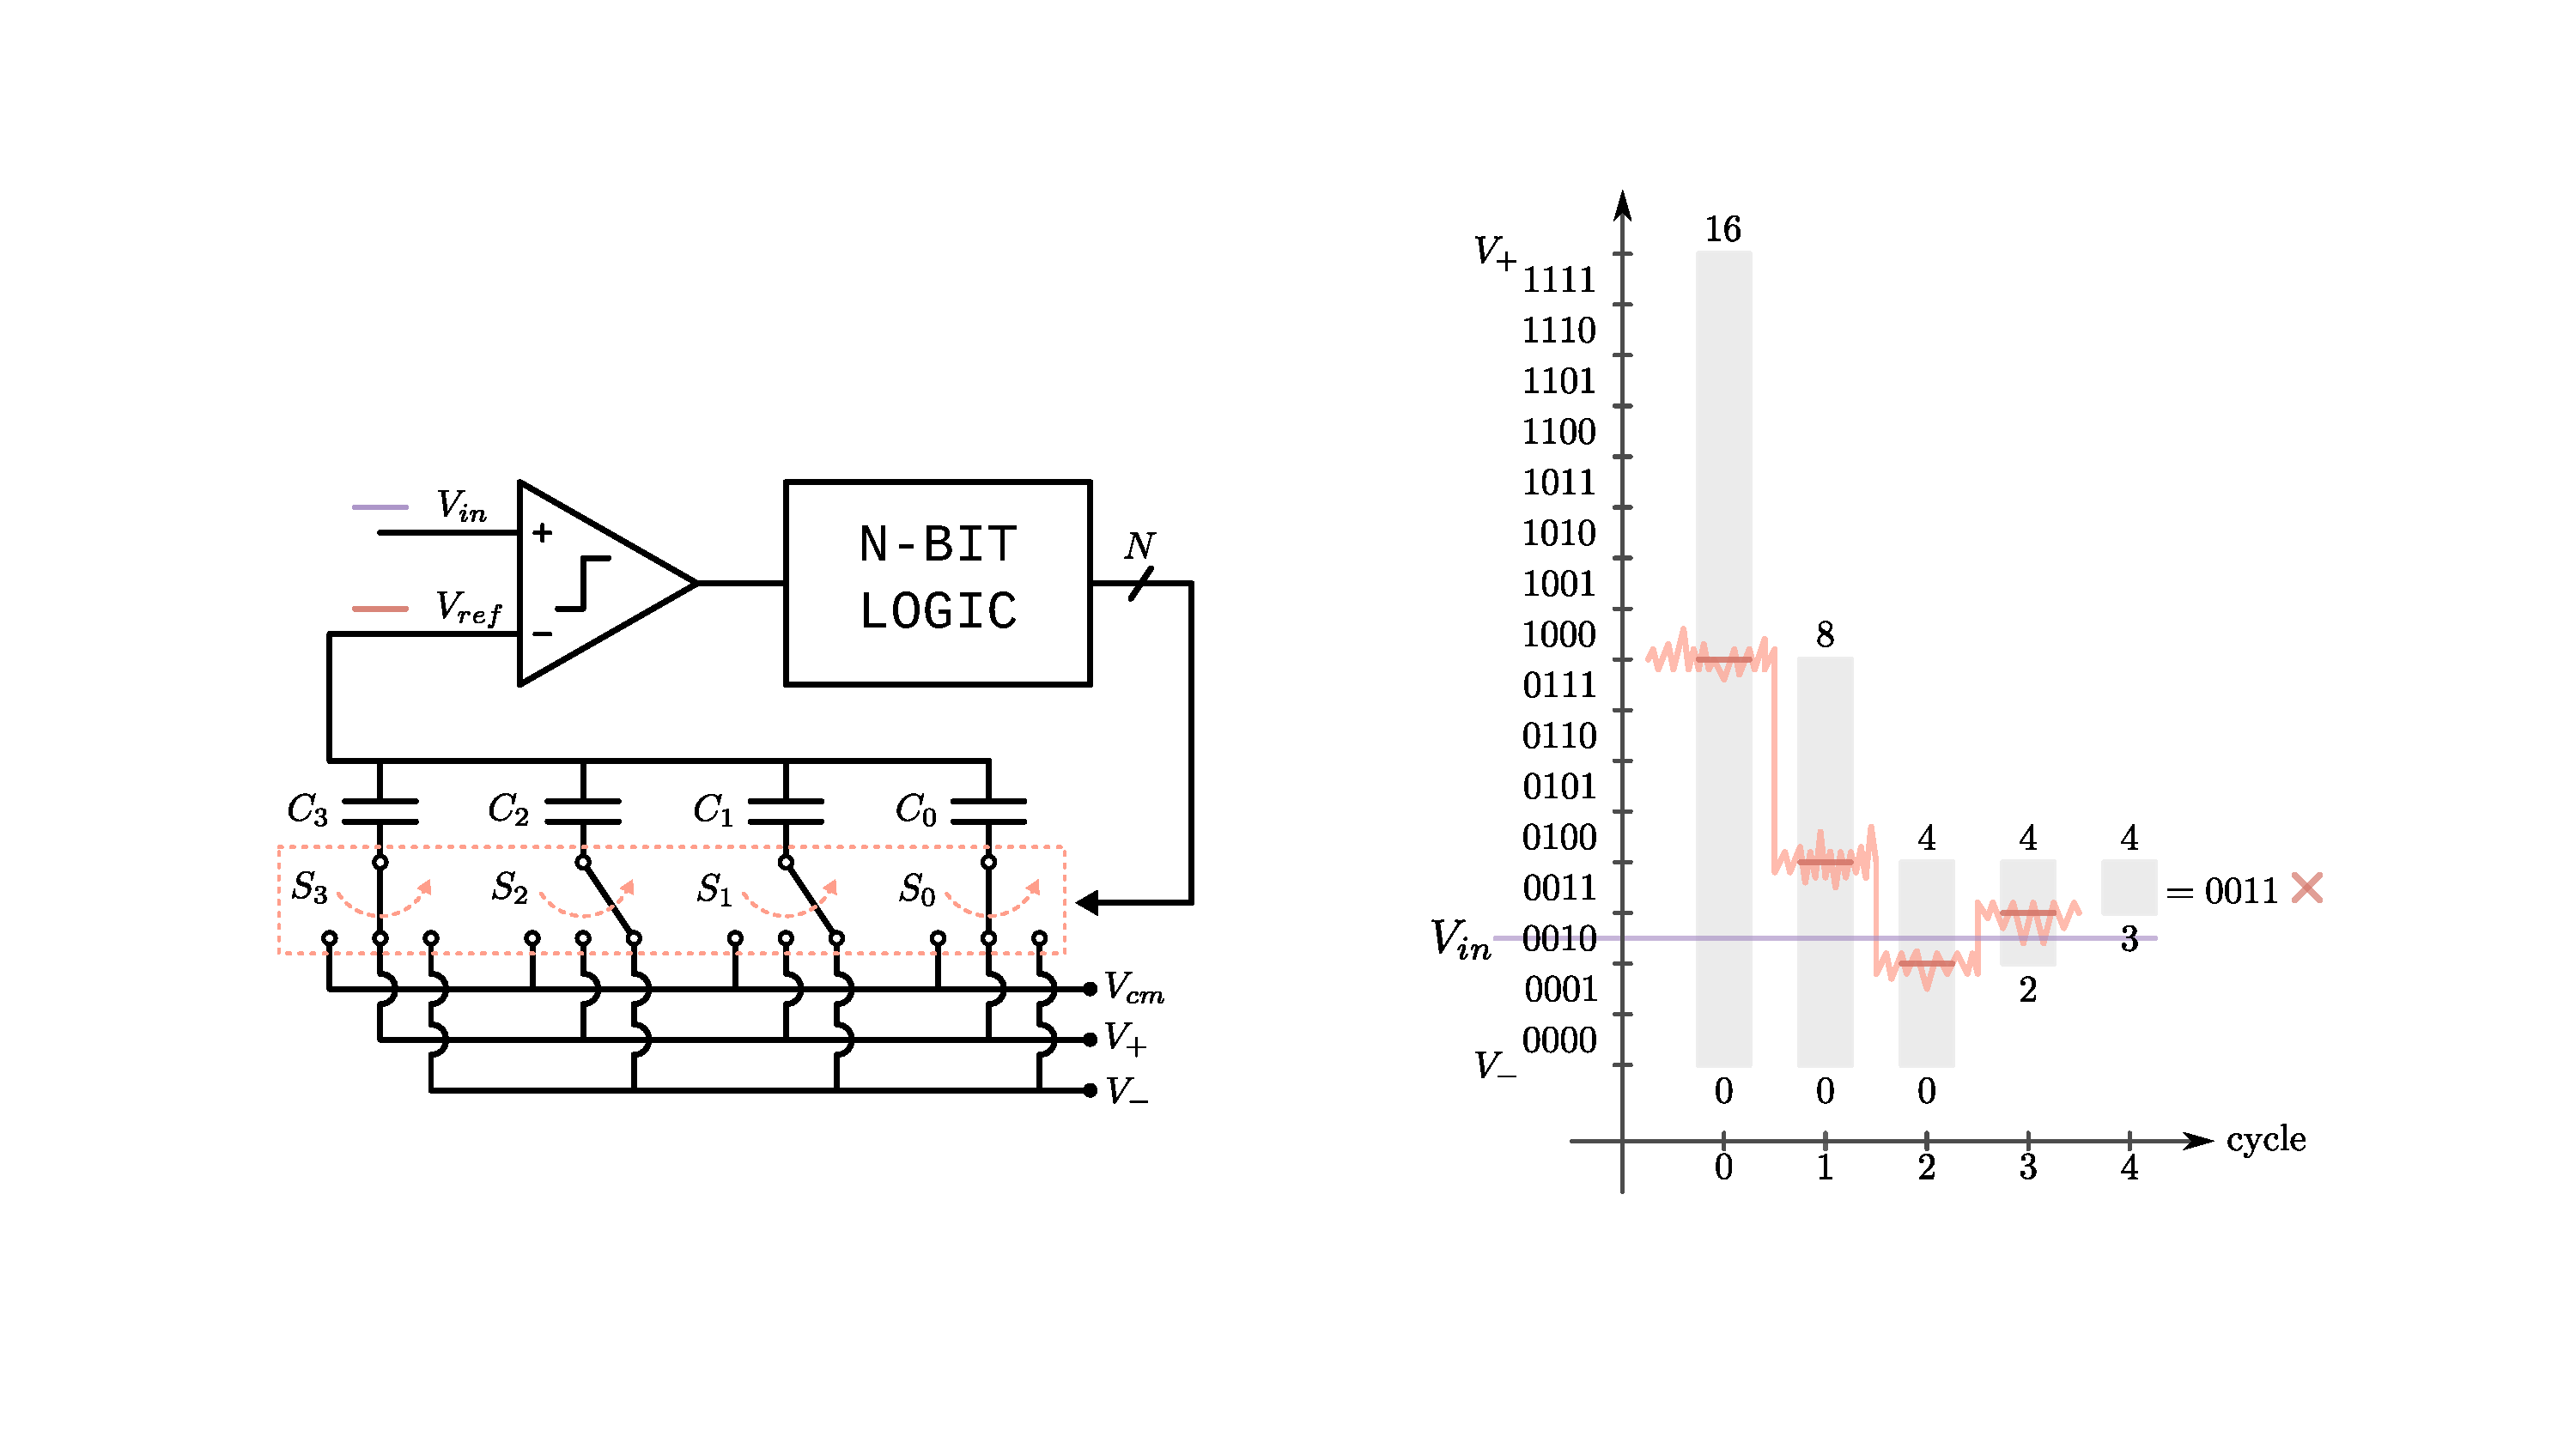
\includegraphics[width=\textwidth]{tranchar3.pdf}}

\frame{\frametitle{Settling error (dynamic error)}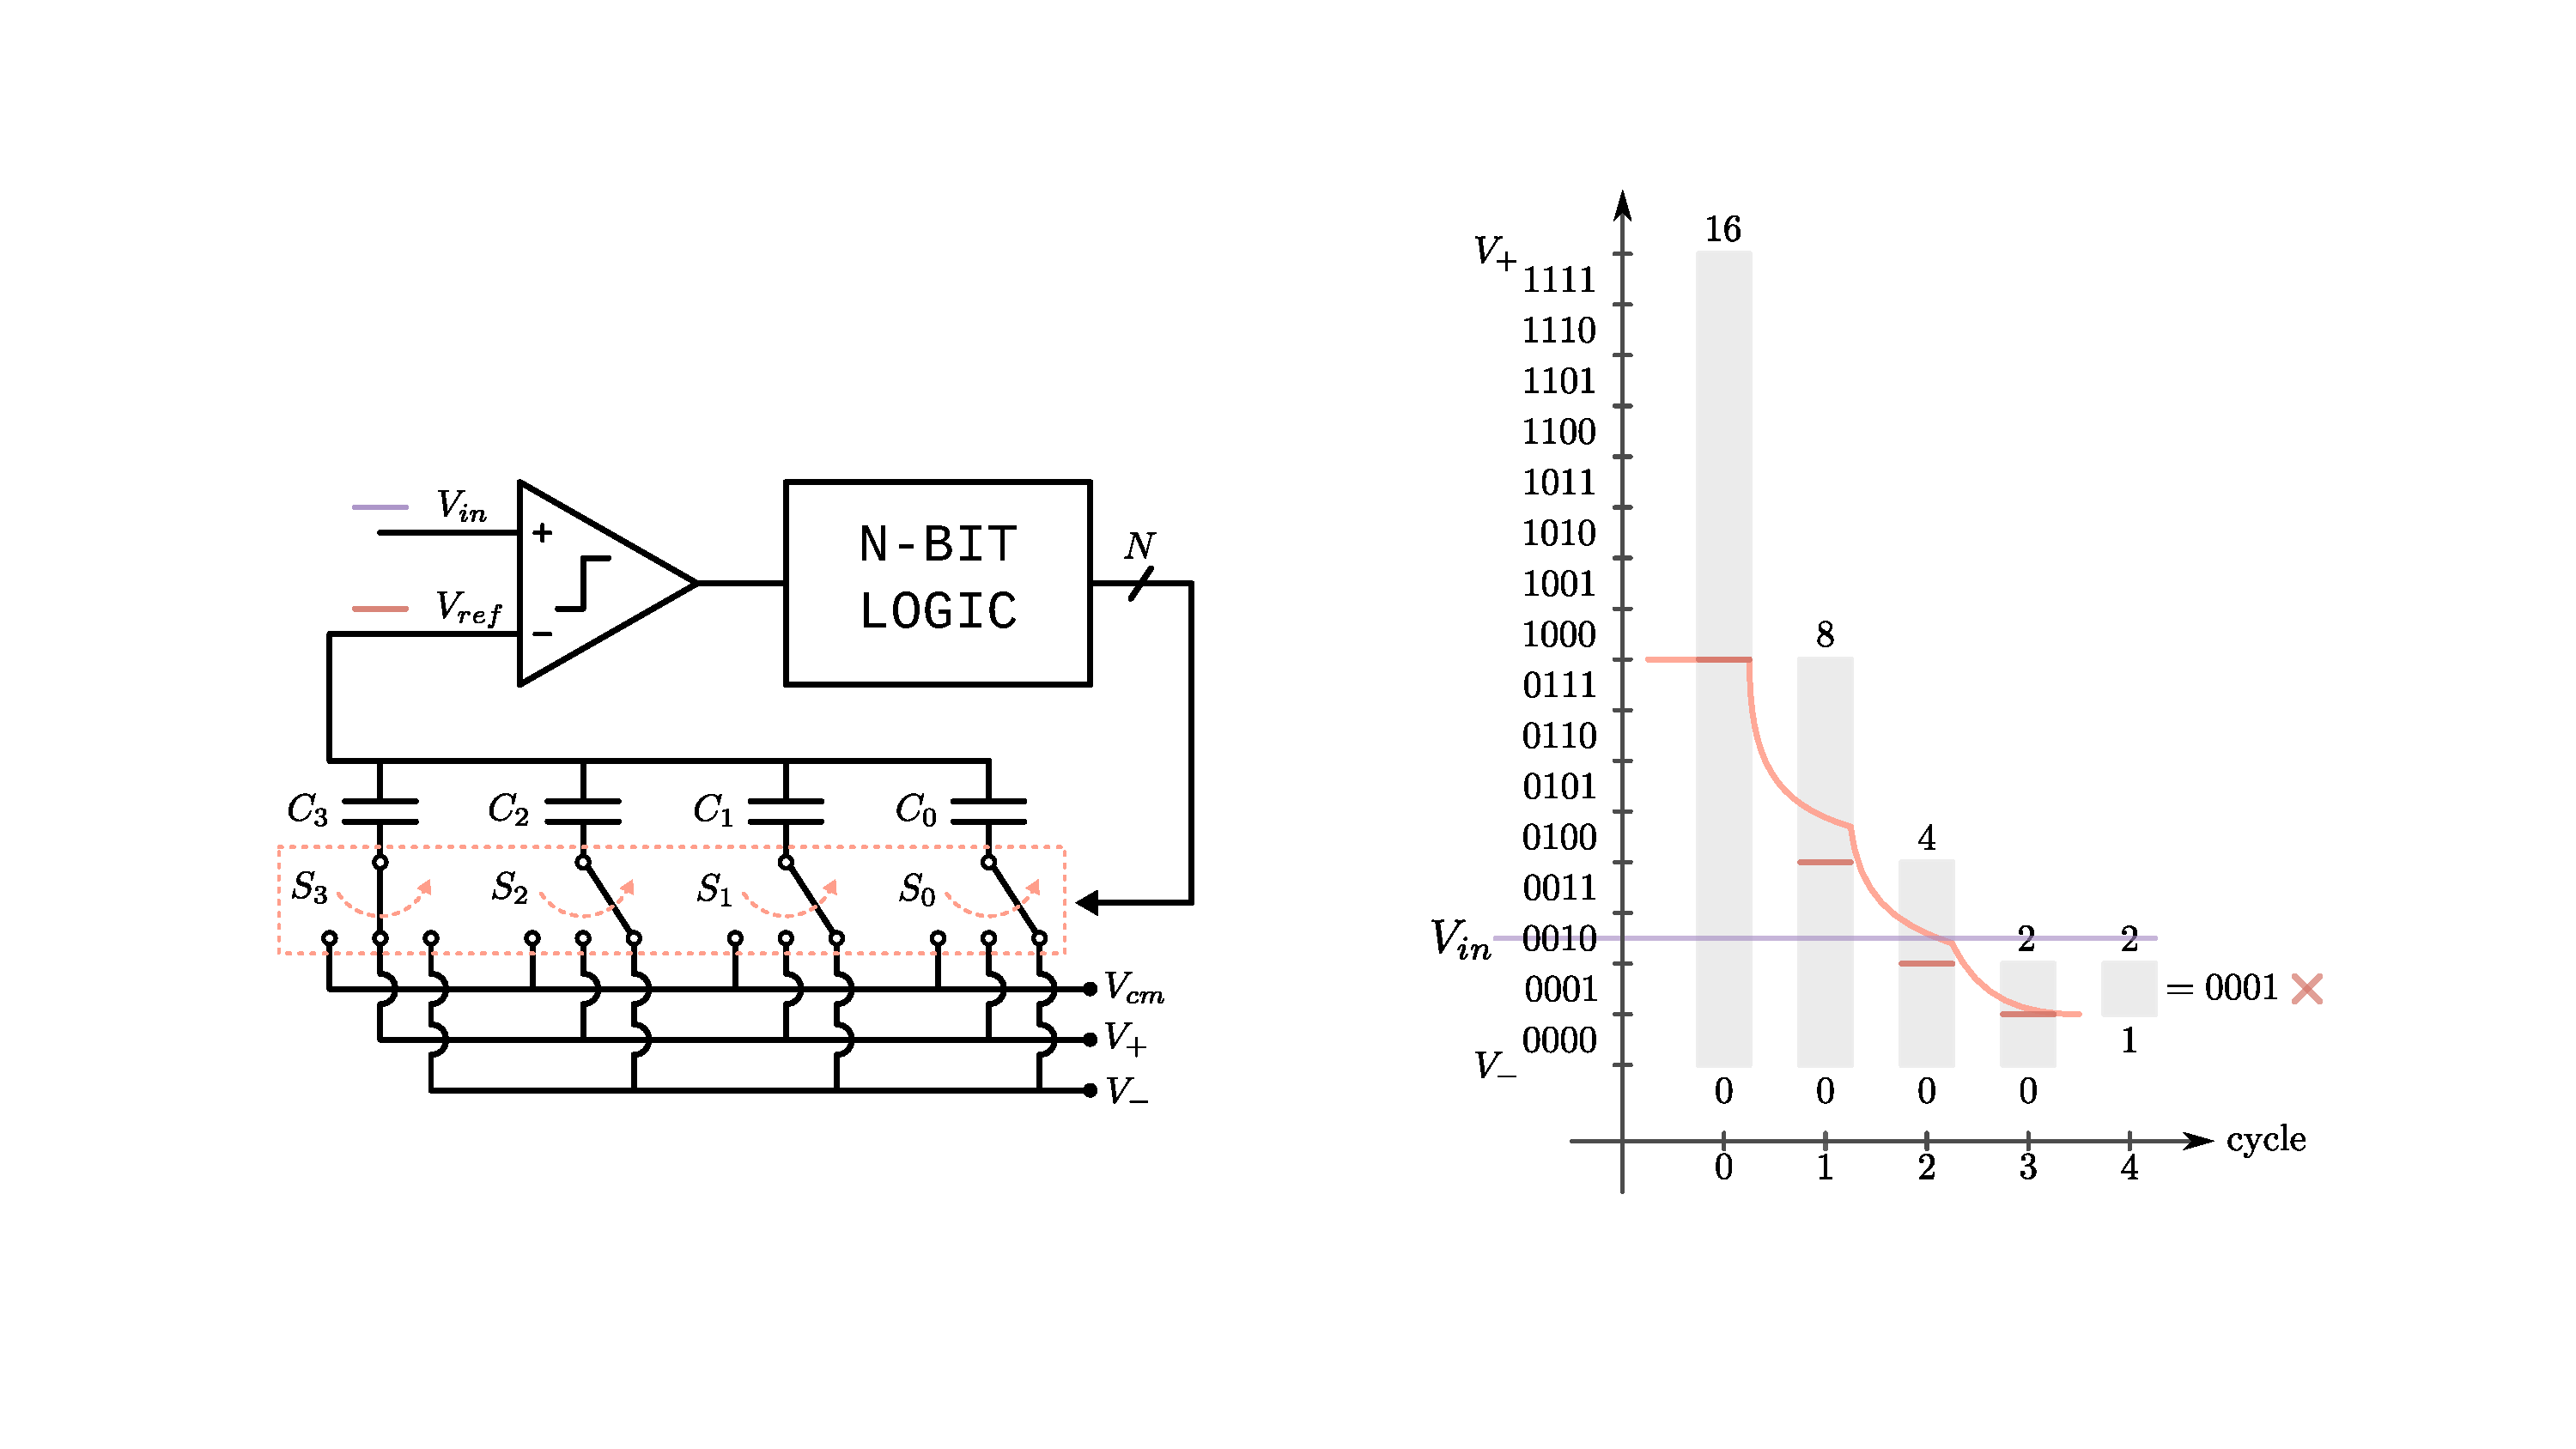
\includegraphics[width=\textwidth]{tranchar2.pdf}}
\frame{\frametitle{Mismatch errors (static error)}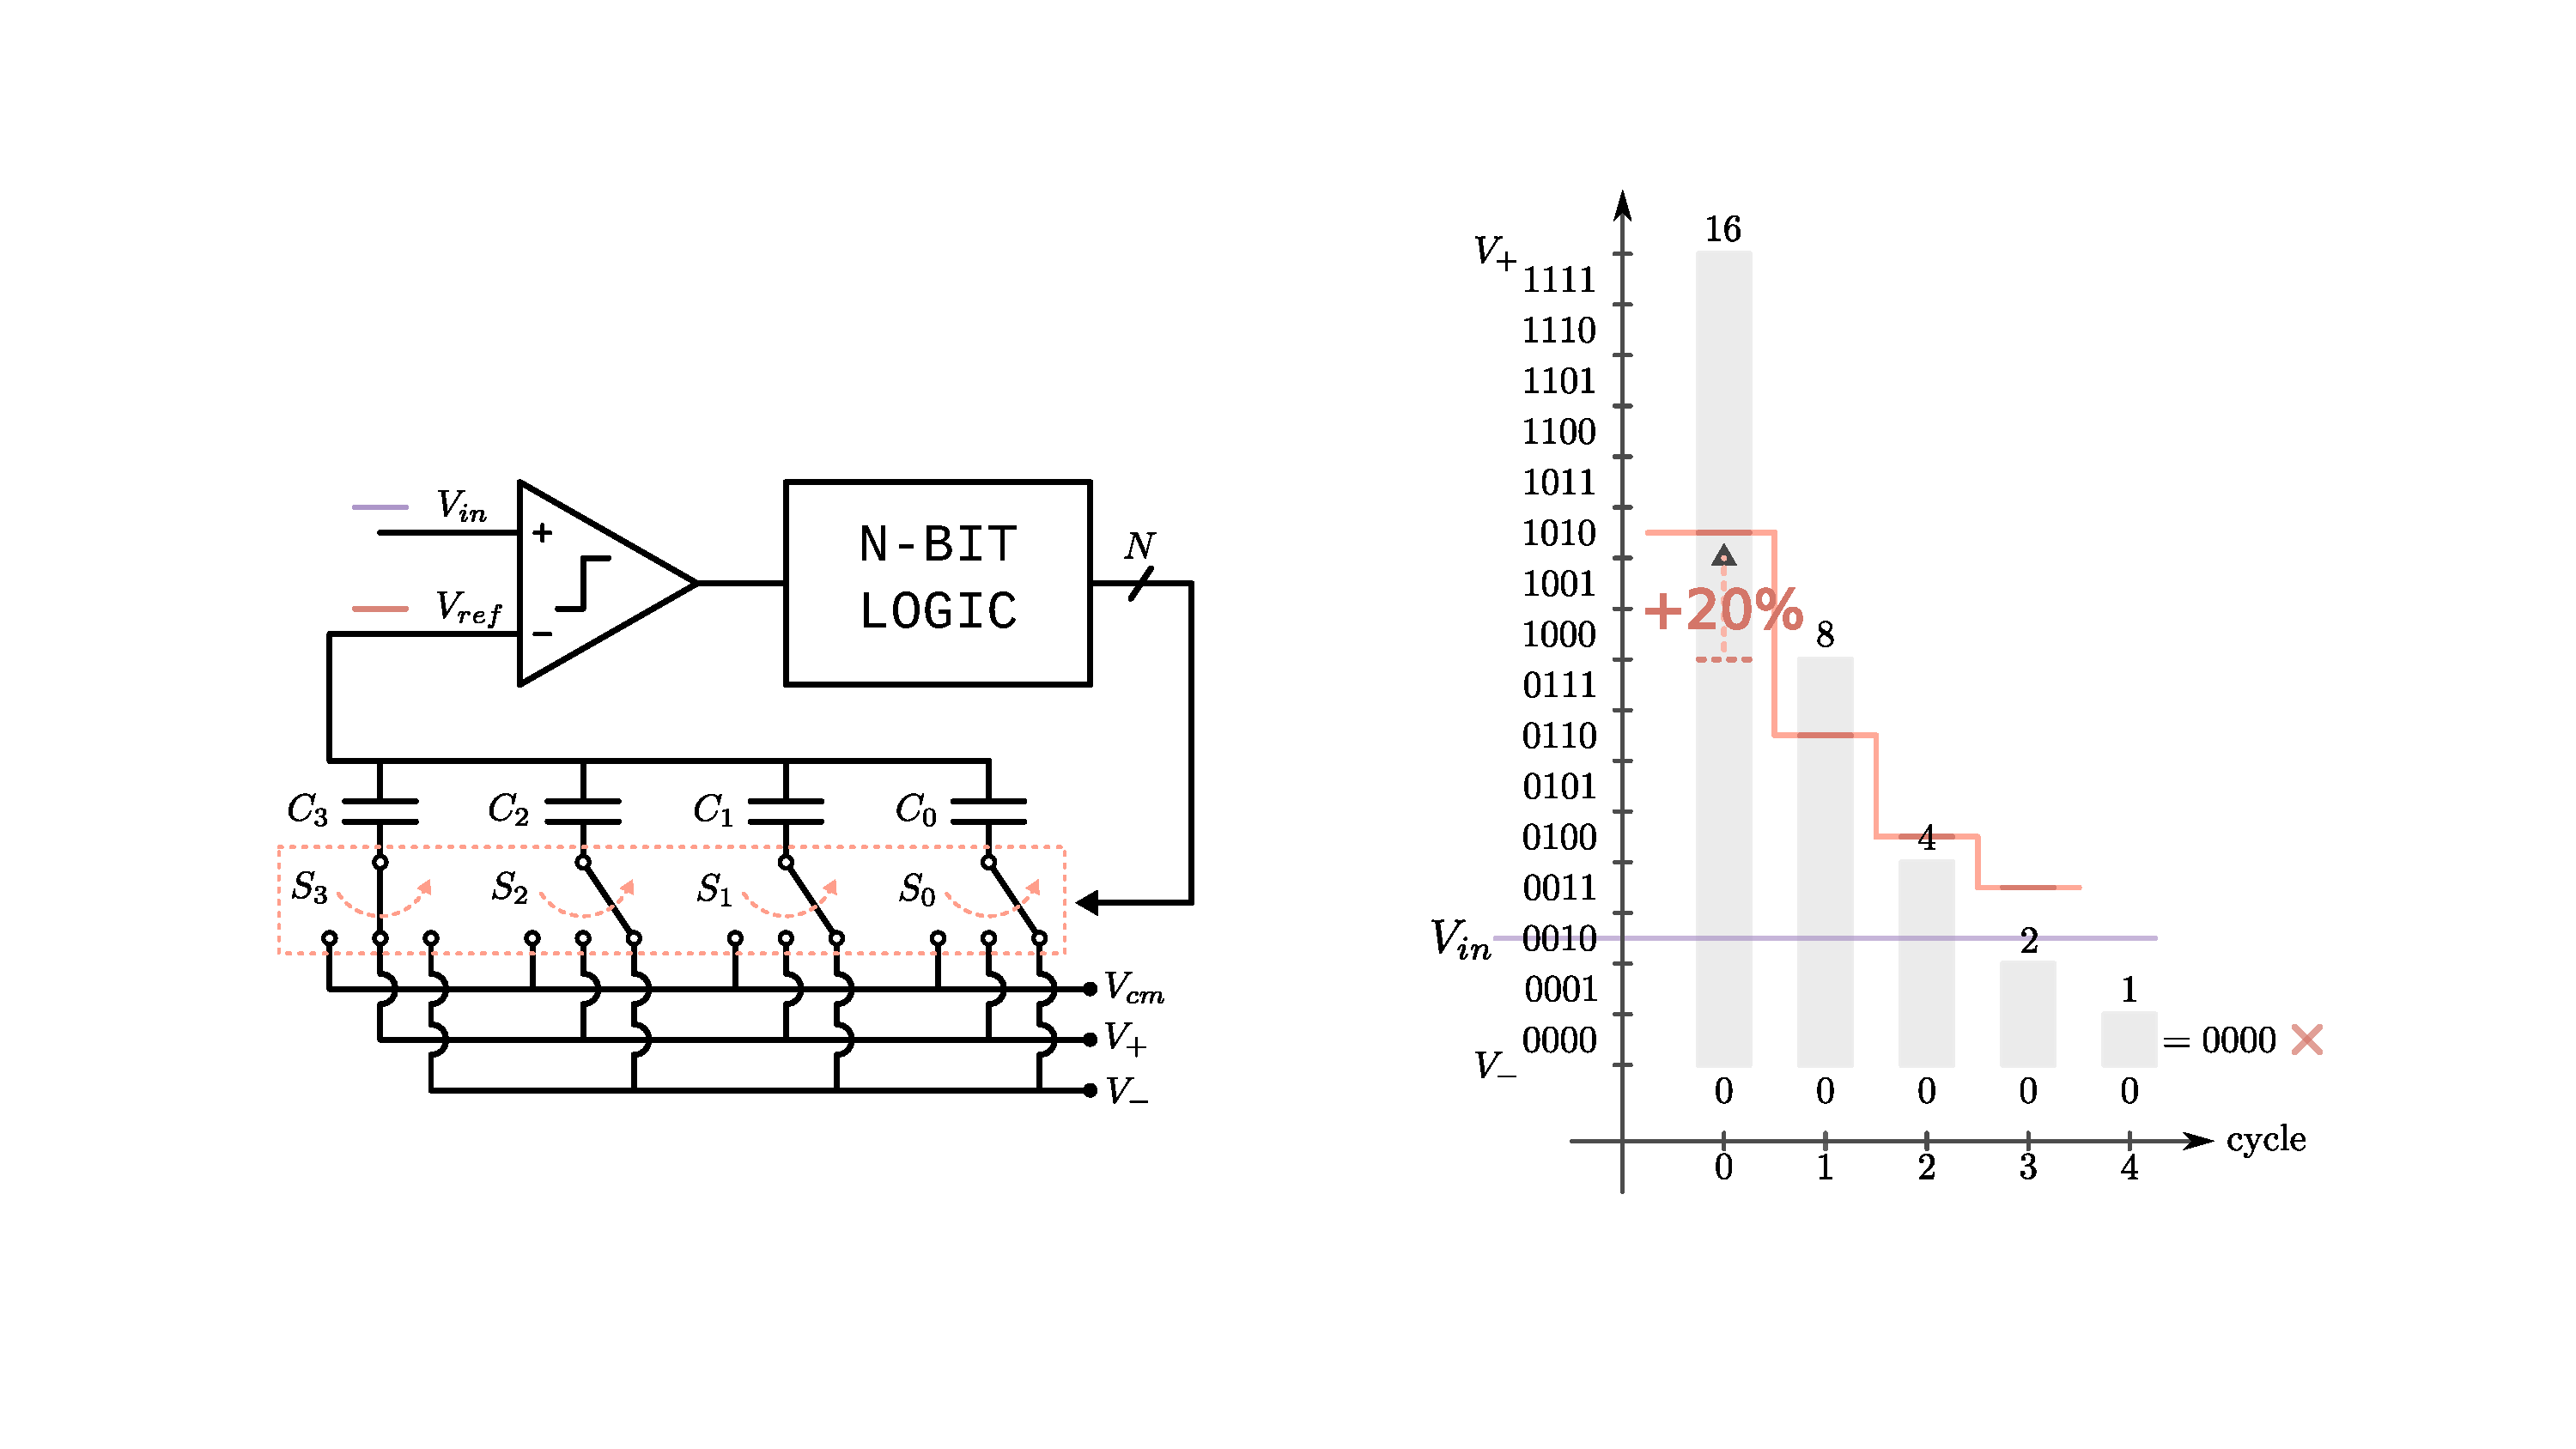
\includegraphics[width=\textwidth]{tranchar4.pdf}}


\begin{frame}
  \frametitle{CDAC construction principles}
  For complete capacitor array. We'd like to be as close to min capacitance as possible, to the point that we'd have 125aF for unit caps in 10-bit design
  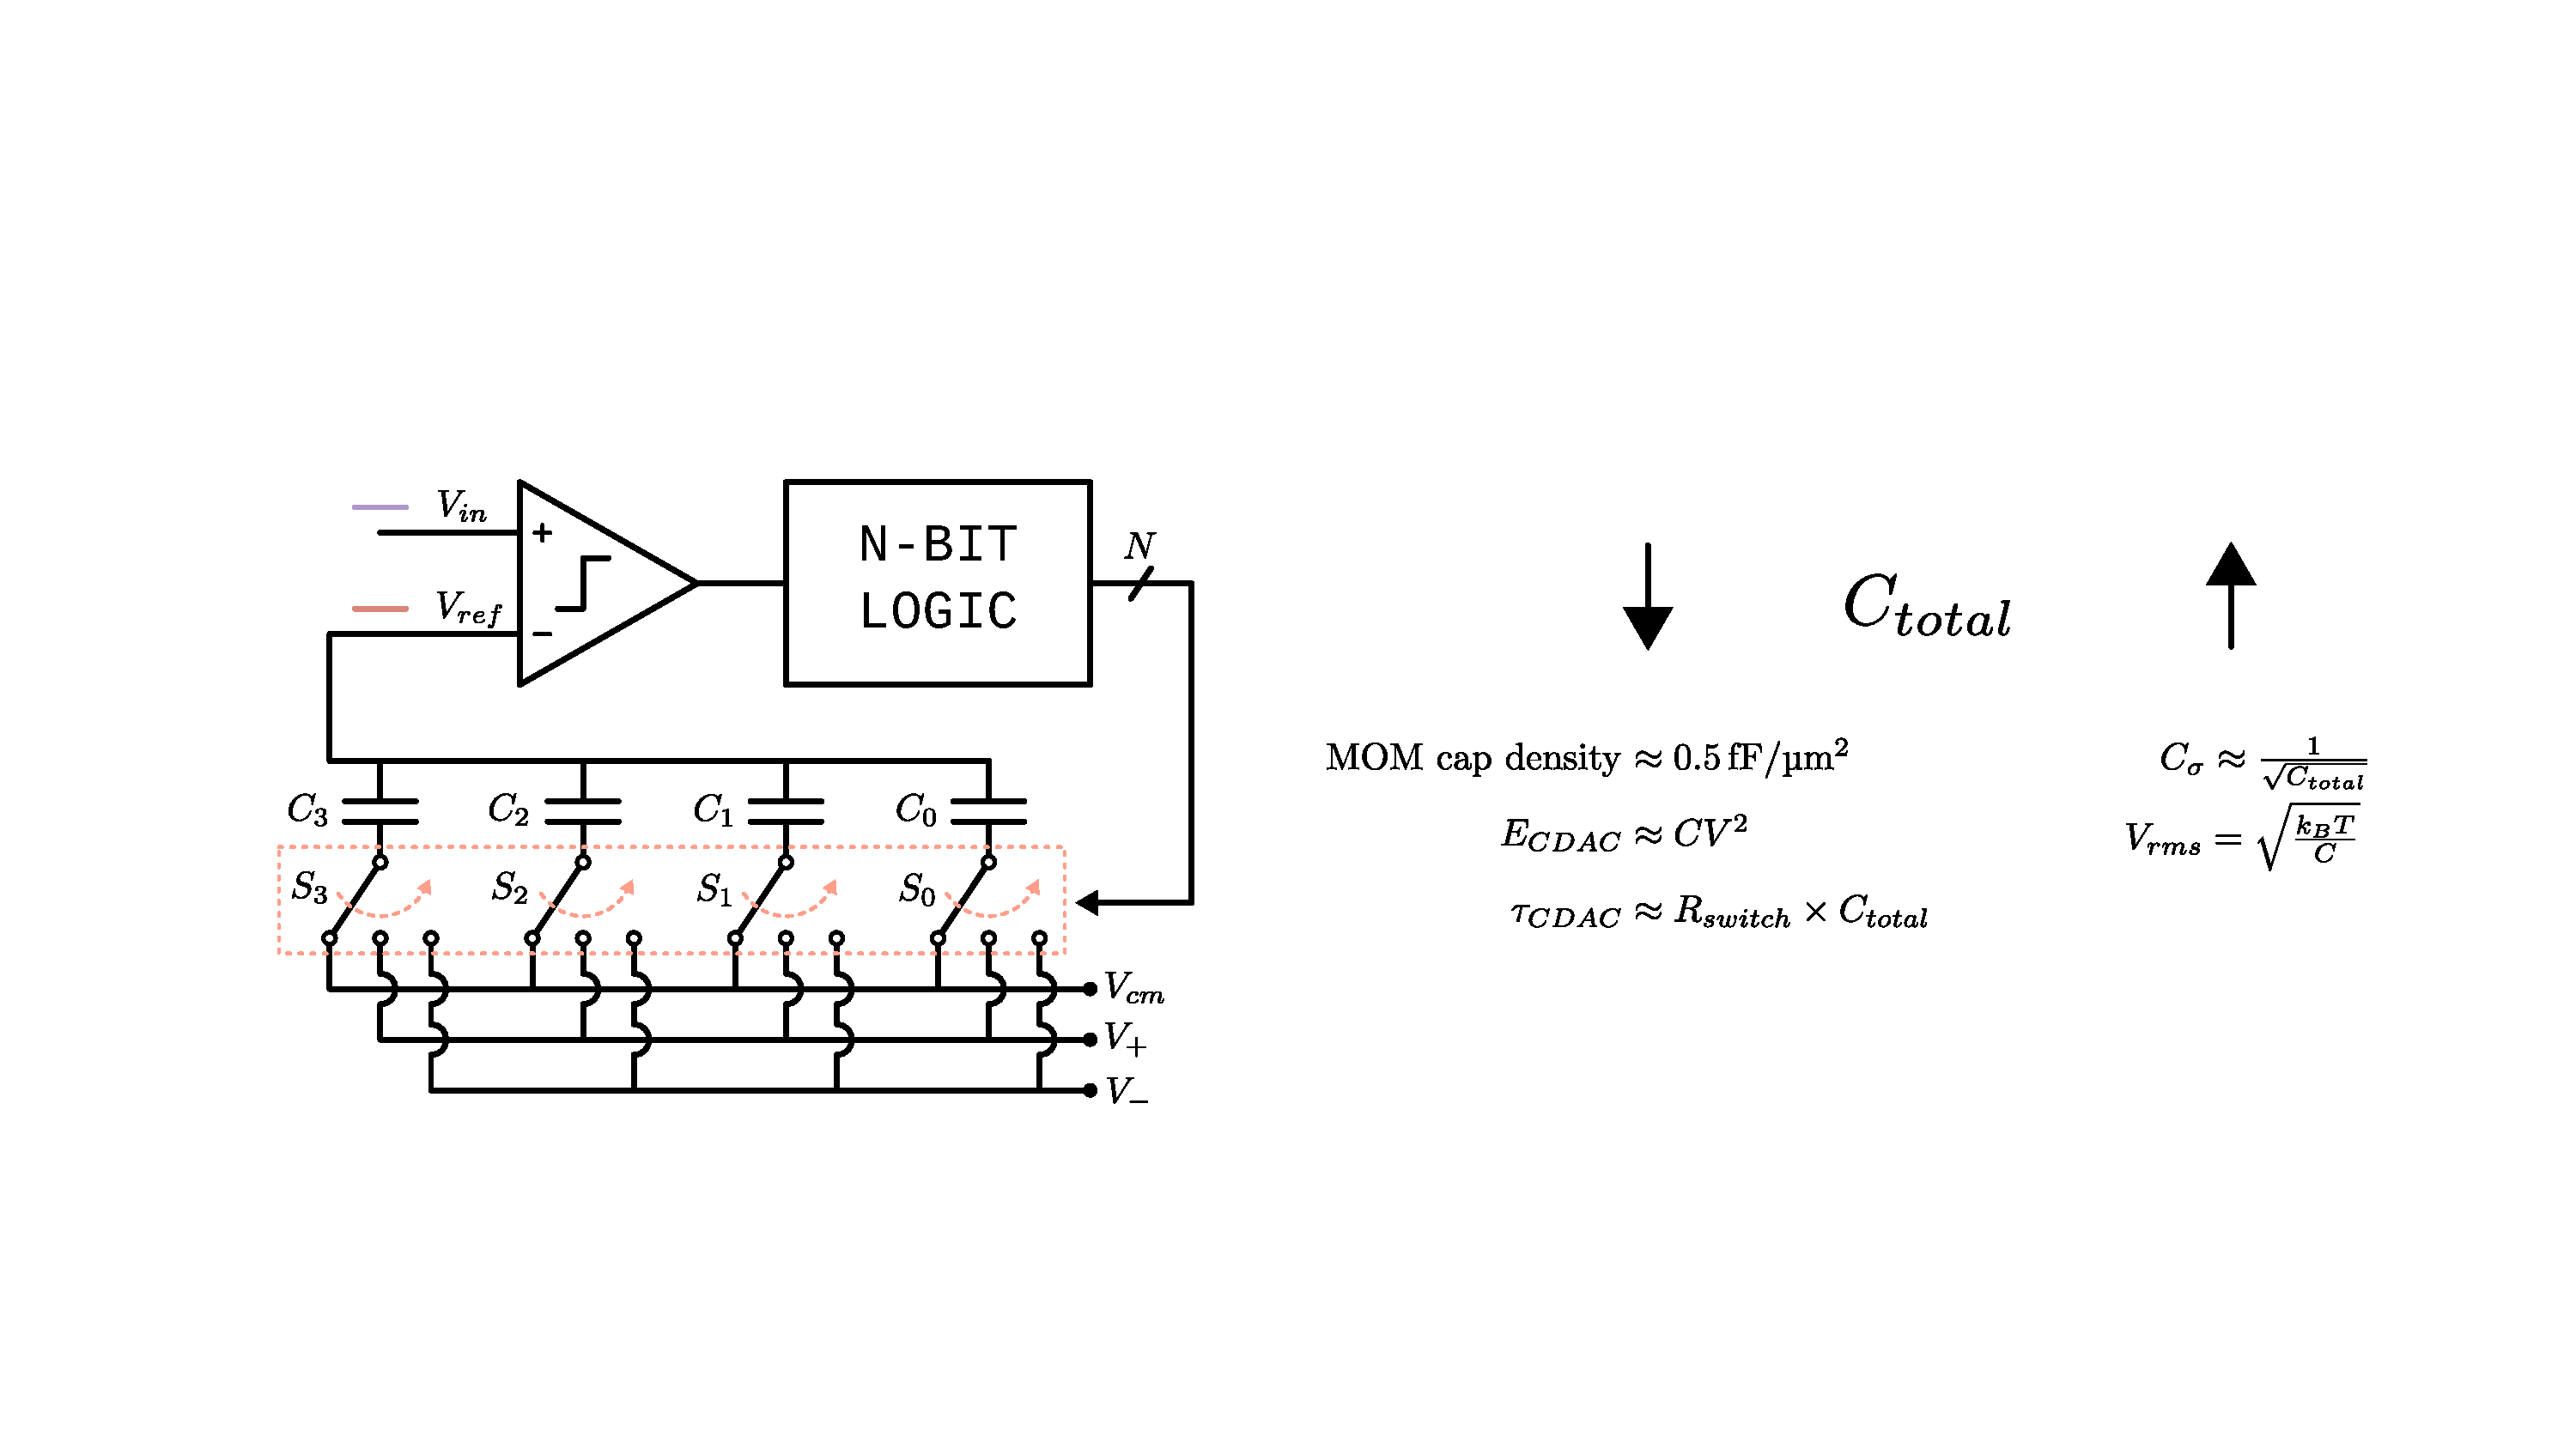
\includegraphics[width=\textwidth]{tranchar5.pdf}
\end{frame}


\begin{frame}
  \frametitle{CDAC construction principles}
  For individual capacitor weights
  \begin{itemize}
    \item Defining each bit weights as integers simplifies cap implementation; improves matching
    \item And defining each bit weight as sum of binary scaled values keeps DEC to just adders
    \item Finally, keeping sum total to binary scaled total prevents overflow
  \end{itemize}
  \end{frame}



\begin{frame}
  \frametitle{SAR modeling status}
  \begin{itemize}
    \item Threshold noise and variation, reference noise, settling error, capacitor mismatch supported
    \item Arbitrary CDAC weights, with support for "extended range bits"
    \item Monotonic and bidirectional-single-side switching supported (CRS, CAS, MCS to be added)
    \item Analyses for static and dynamic performance analyses ($ENOB @ f_{s}$)
    \item Single test case requires 20 seconds
    \item Compatibility with T-Spice, AFS, and Spectre simulator (30hr run, 4hr with Spectre)
  \end{itemize}

\end{frame}
\begin{frame}
    \frametitle{SAR modeling status}
  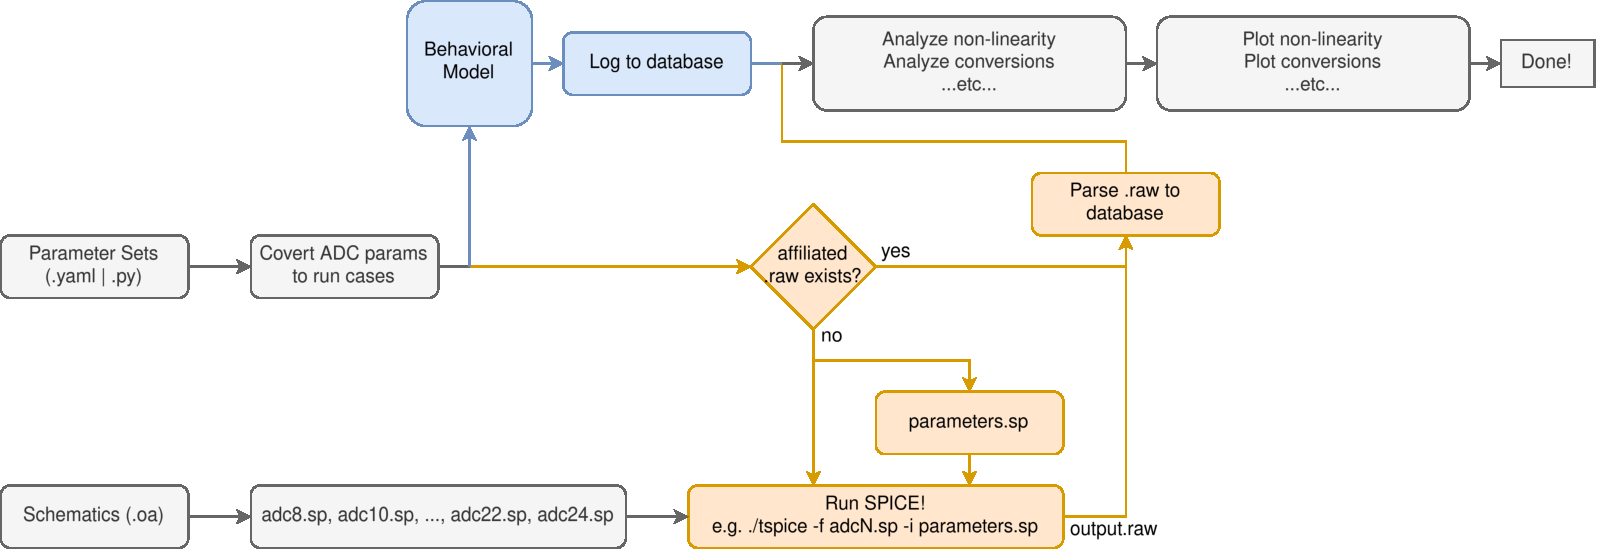
\includegraphics[width=\textwidth]{workflow.pdf}
\end{frame}

\frame{\frametitle{Ideal 10-bit operation}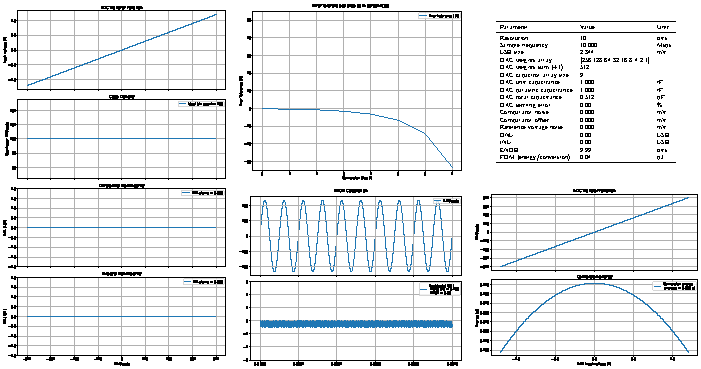
\includegraphics[width=\textwidth]{behavioral_10b_ideal_combine.pdf}}

\begin{frame}
  \frametitle{Error tolerance strategies}
  Sub-radix 2 steps
  \begin{itemize}
    \item Creates overlapping search voltages
    \item In $D_{out}$ procesed as $W_i \times B_i$
    \item Can also satisfy calibratability requirements
  \end{itemize}
  Extended search steps
  \begin{itemize}
    \item In $D_{out}$ procesed as $W_i \times (B_i-0.5)$
    \item Decreases input amplitude swing to $V_{ref} \times \frac{C}{d}$
    \item Introduced by CC Liu 2010, where they were additional cap, 
  \end{itemize}
  \end{frame}

\begin{frame}
  \frametitle{Error tolerance strategies}
  \begin{center}
    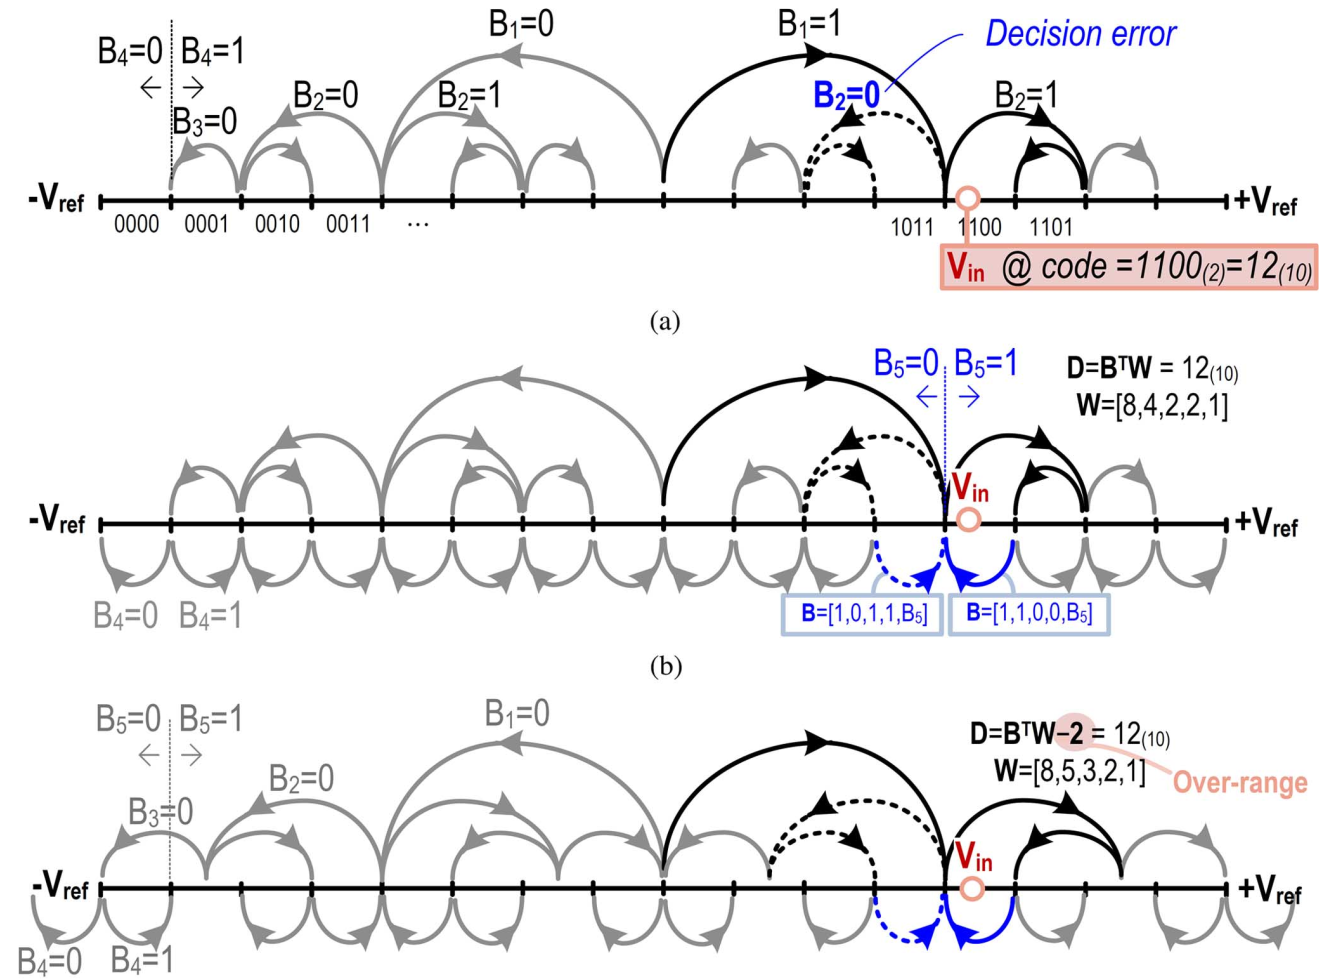
\includegraphics[width=0.6\textwidth]{redun_strats.png}
  \end{center}
  \end{frame}


\begin{frame}
\frametitle{Device and reference noise correction}
\begin{itemize}
  \item In most common case, only small LSBs errors will occur from thermal noise.
  \item Can be corrected by single post-bits, or more comparator power
\end{itemize}
\begin{equation*}
\sigma_n^2 \leq LSB^2 / 2 \times 12
\end{equation*}
\begin{center}
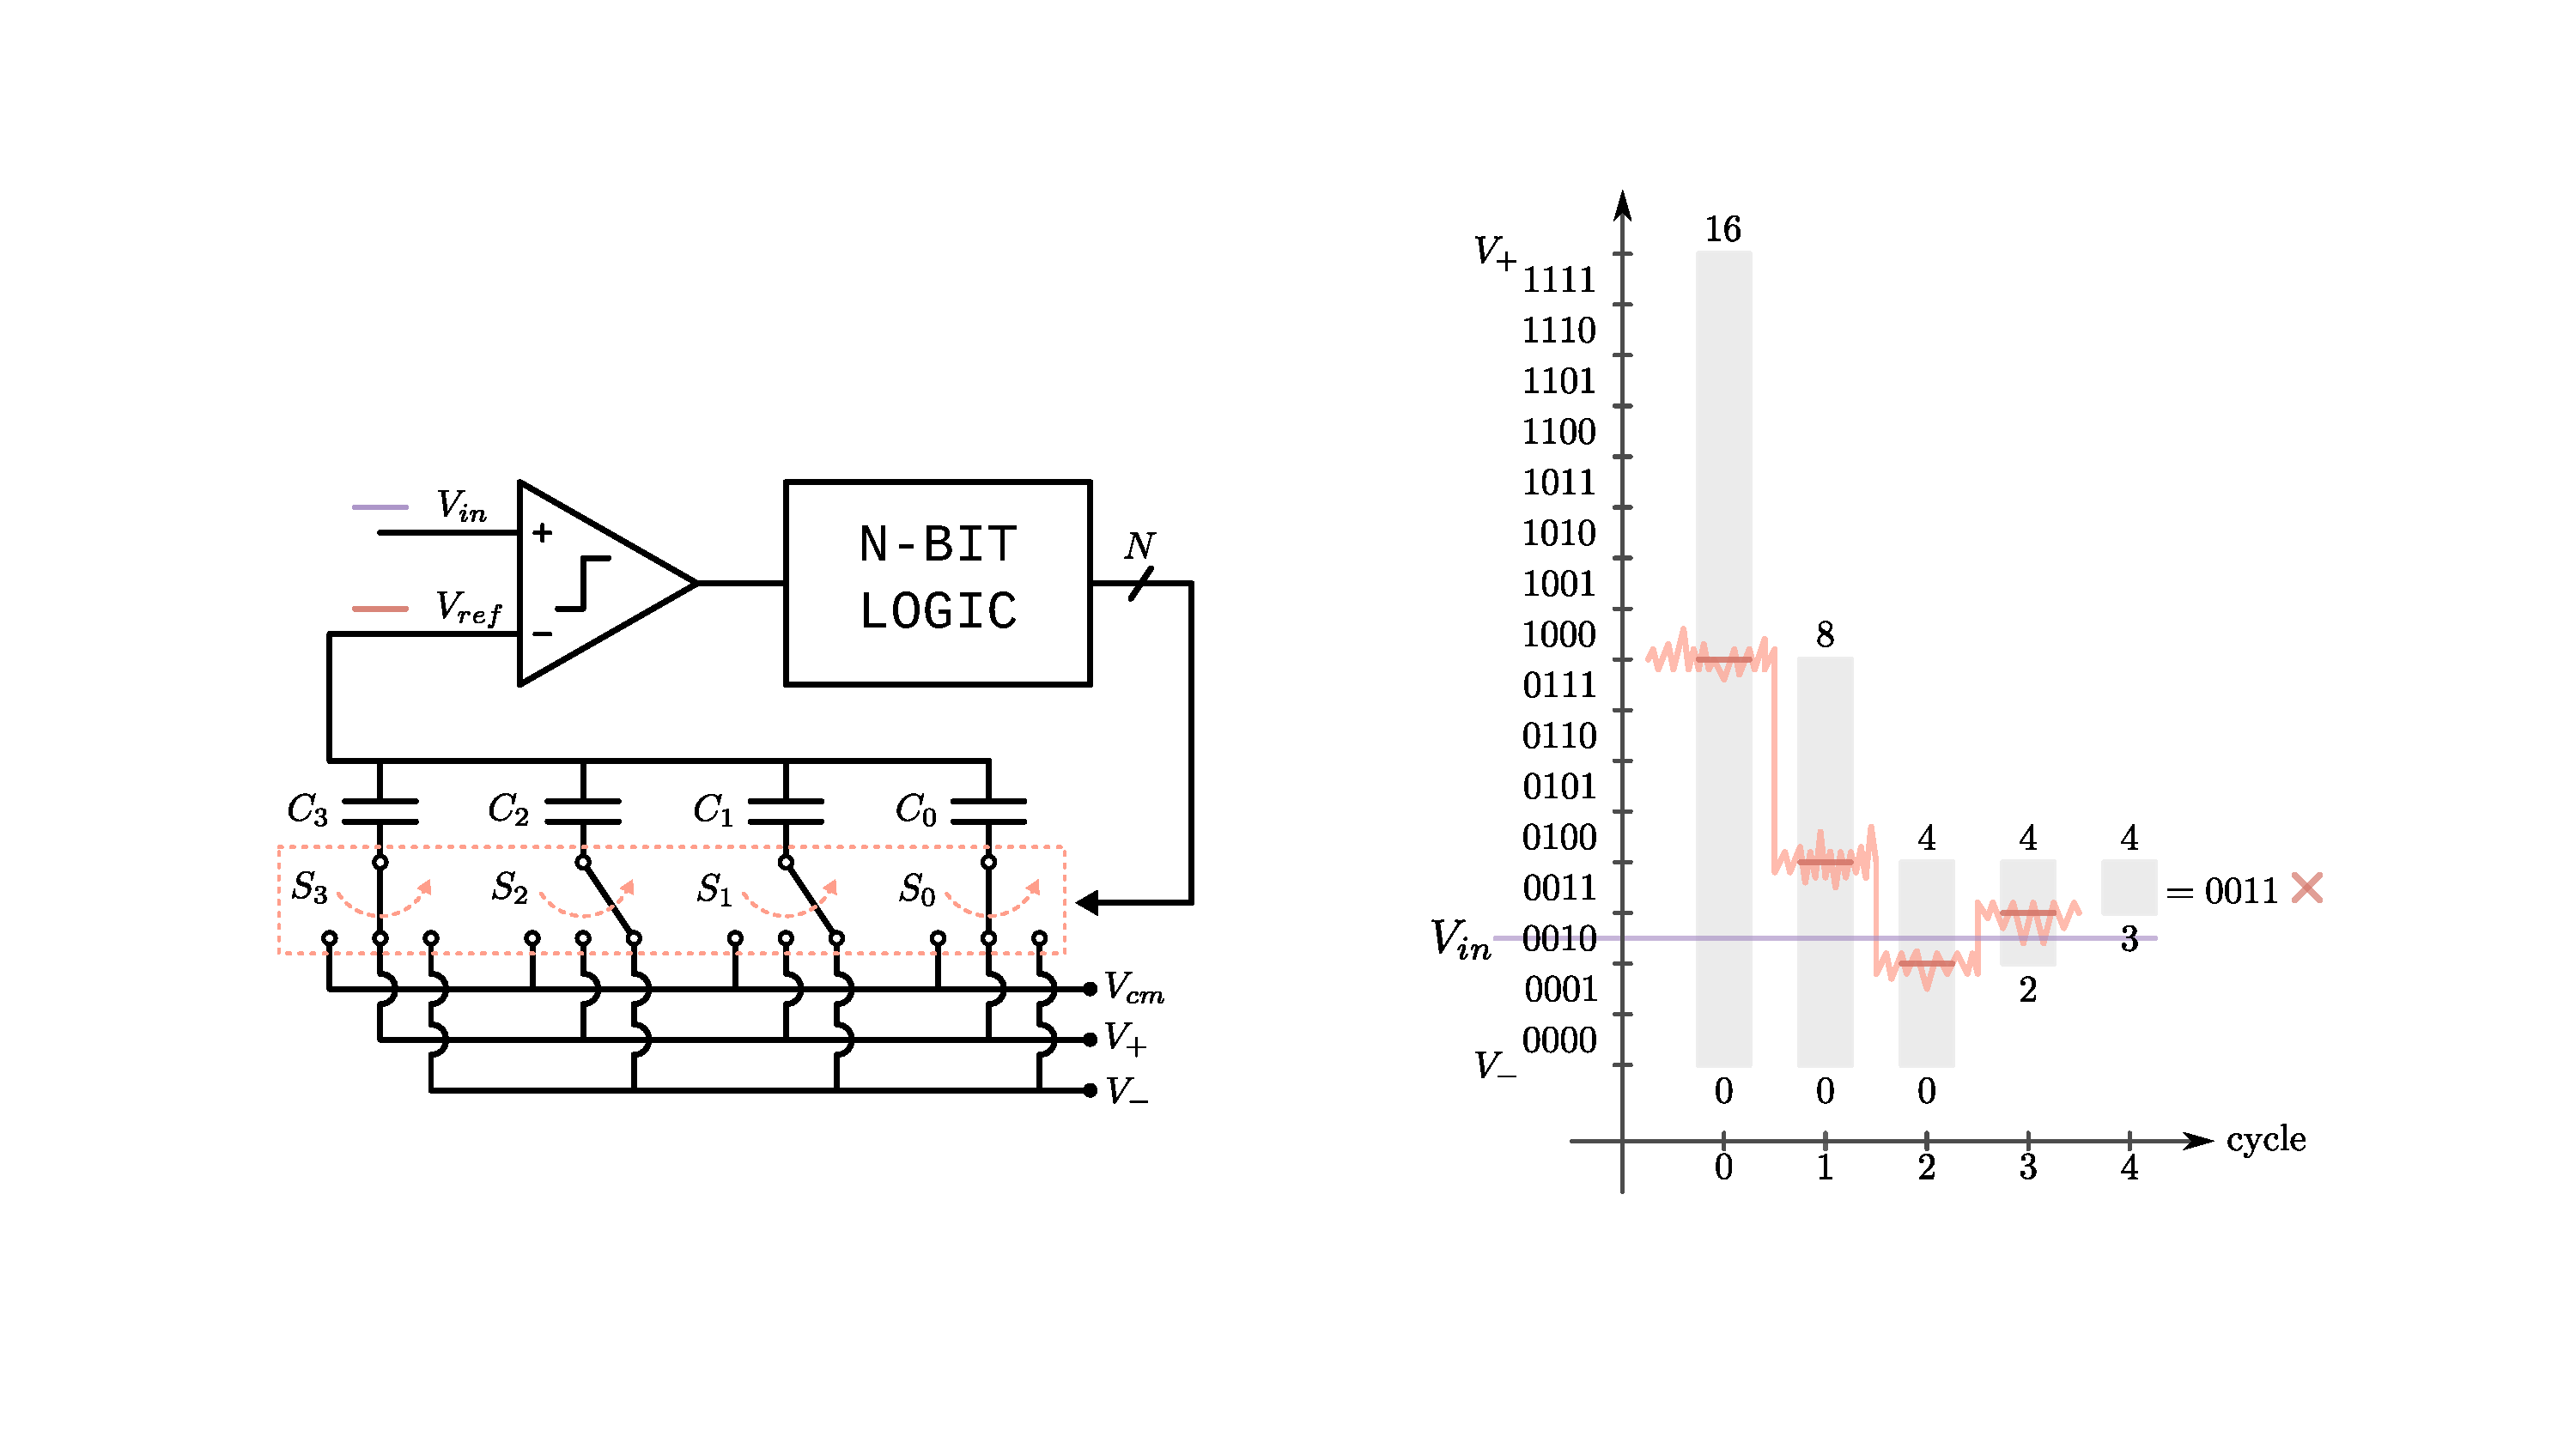
\includegraphics[width=0.6\textwidth]{tranchar3.pdf}
\end{center}
\end{frame}

\begin{frame}
\frametitle{Settling error correction}
Most pronounced in MSBs, recovery determined by remaining caps:
\begin{equation*}
\textrm{Error tolerance @} B_i = \frac{\sum_{i+1}^{M}B_j - B_i} {\sum_{i}^{M}B_j} \times 100 \%
\end{equation*}
\begin{center}
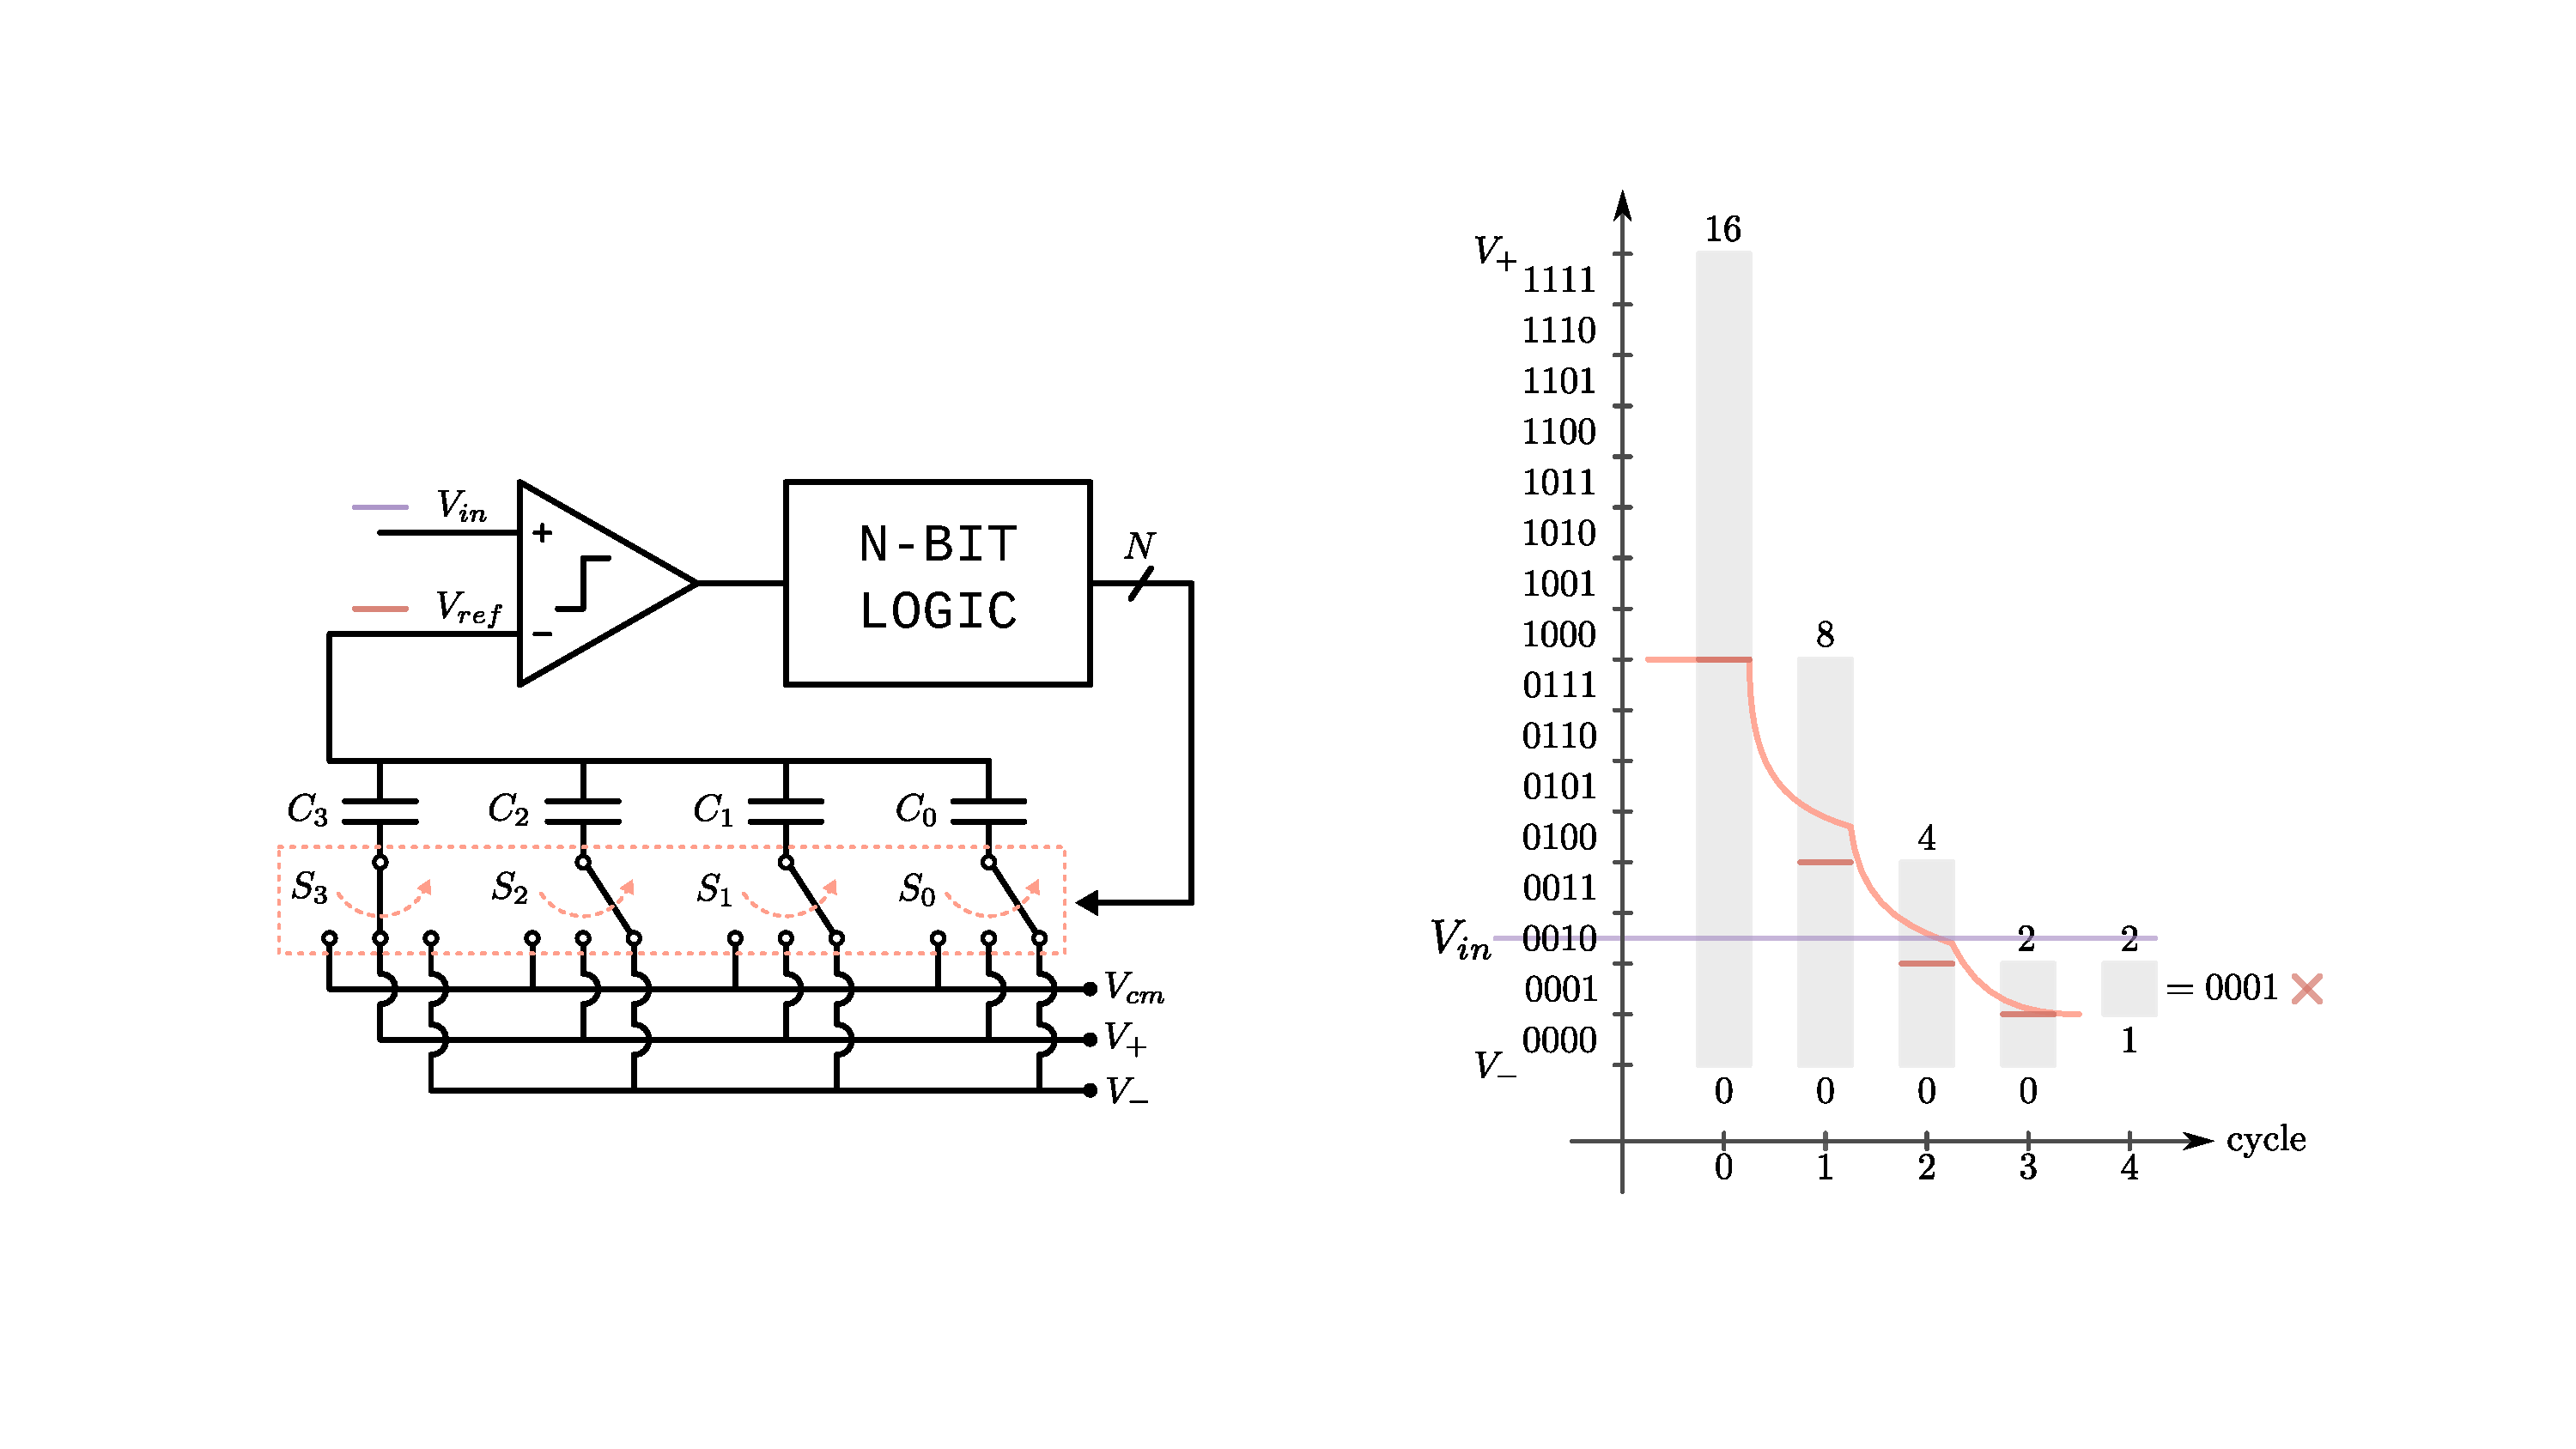
\includegraphics[width=0.6\textwidth]{tranchar2.pdf}
\end{center}
\end{frame}

\begin{frame}
\frametitle{Mismatch static error \& calibratability}
\begin{itemize}
  \item Redundancy can absorb static error, but what about mismatch?
  \item 1-bit comparator = inherintely linear, so CDAC dominates
  \item Assuming monotonic switching, without cap-reuse like CRS [Tsai 2015]
\end{itemize}
\begin{equation*}
\sigma_{INL_{max}} \approx \frac{1}{2}(\sigma_{C_{unit}})\sqrt{2^N}
\end{equation*}
  \begin{center}
  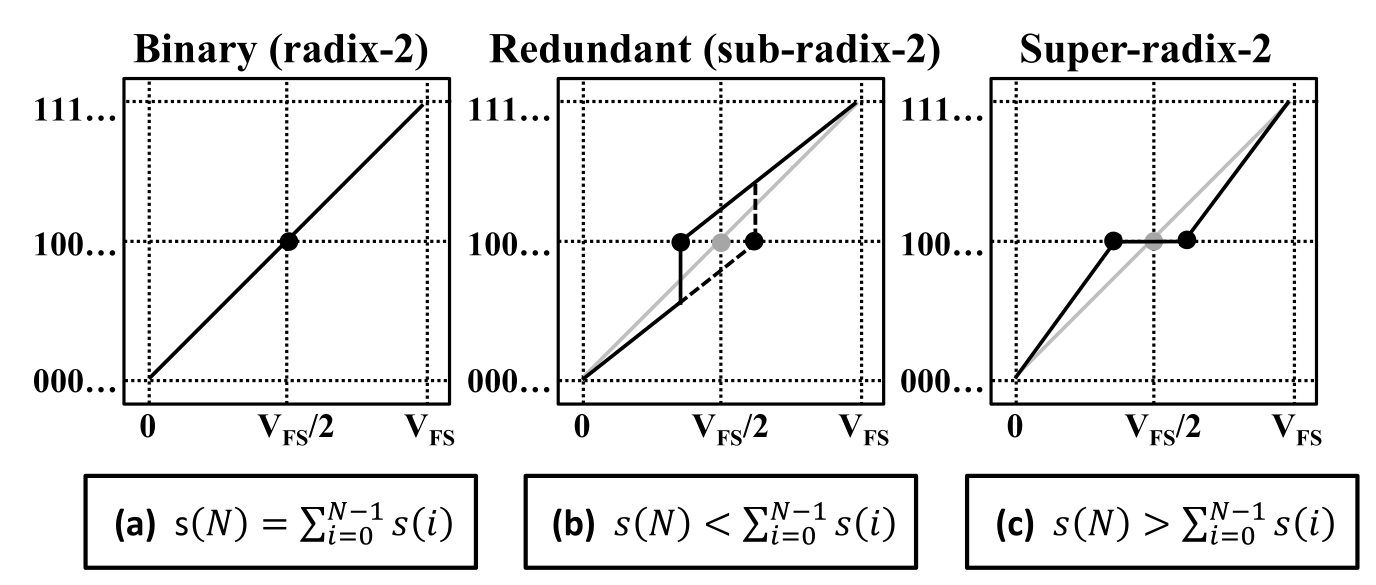
\includegraphics[width=0.6\textwidth]{calibrate.png}
  \end{center}
\end{frame}

\begin{frame}
  \frametitle{Mismatch static error \& calibratability}
    \begin{center}
    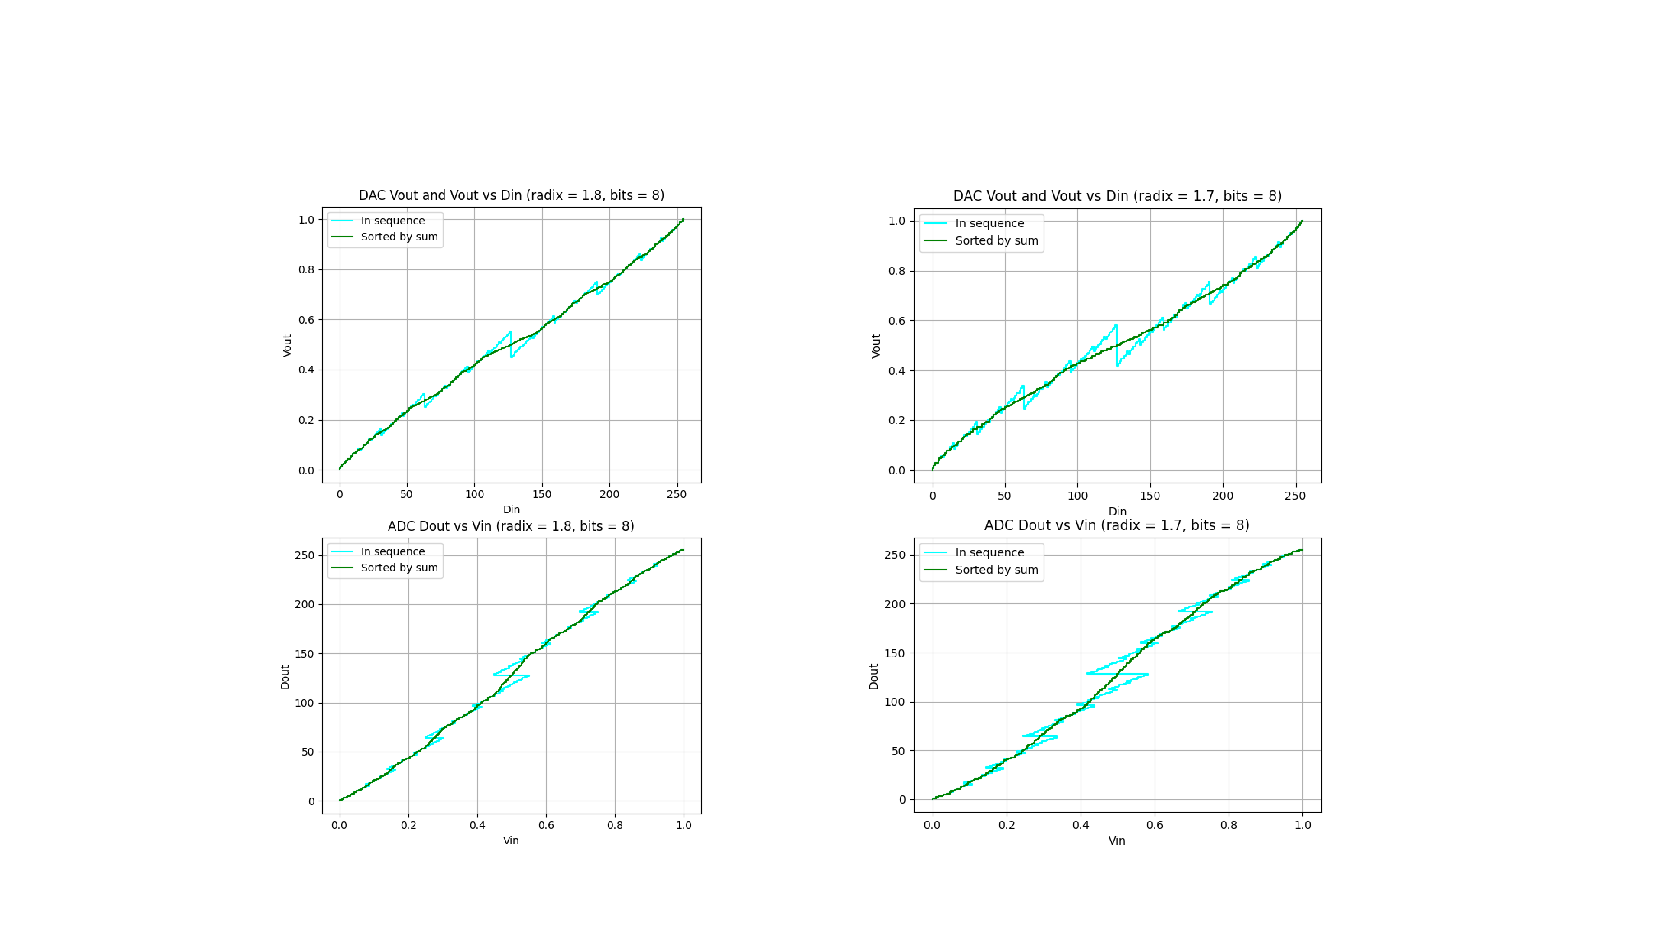
\includegraphics[width=\textwidth]{overlap.pdf}
    \end{center}
  \end{frame}

\frame{\frametitle{10-bit w/ device noise}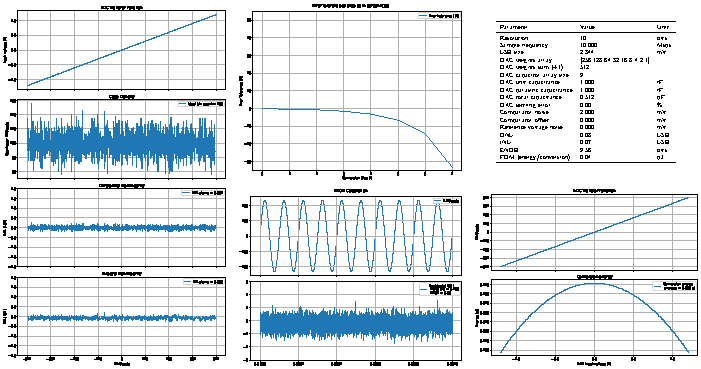
\includegraphics[width=\textwidth]{behavioral_10b_devnoise_combine.pdf}}
\frame{\frametitle{10-bit w/ reference noise}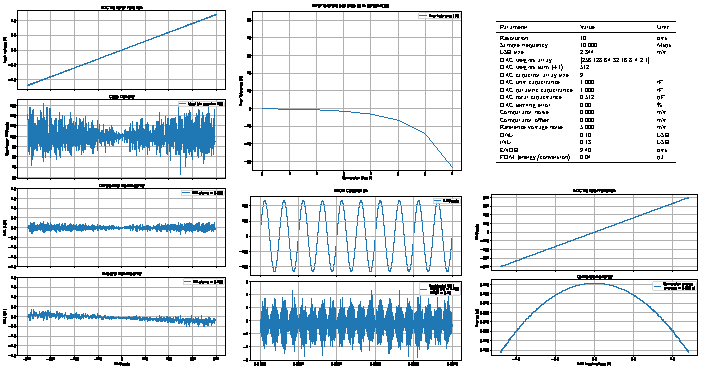
\includegraphics[width=\textwidth]{behavioral_10b_refnoise_combine.pdf}}
\frame{\frametitle{10-bit w/ device and reference noise}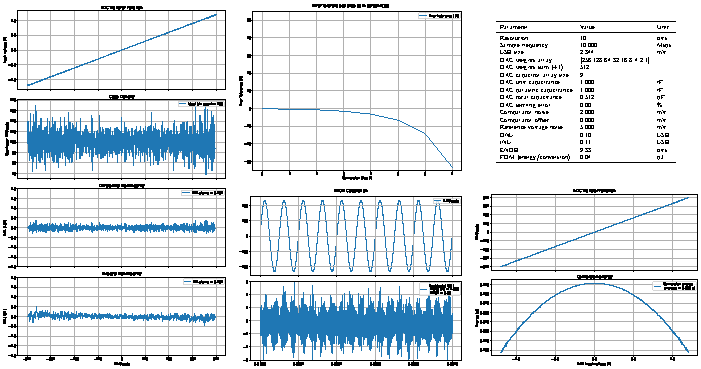
\includegraphics[width=\textwidth]{behavioral_10b_noisy_combine.pdf}}


% \frame{\includegraphics[width=\textwidth]{behavioral_10b_noisy_postconv.pdf}}
% \frame{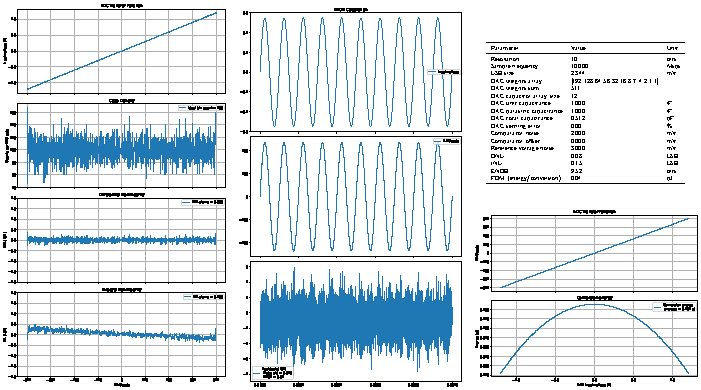
\includegraphics[width=\textwidth]{behavioral_10b_noisy_scadec_combine.pdf}}
% \frame{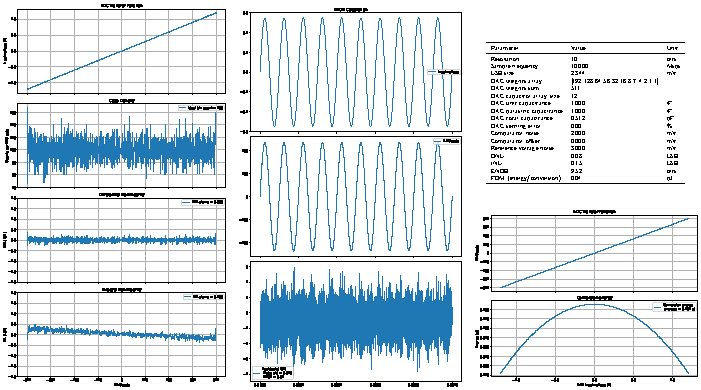
\includegraphics[width=\textwidth]{behavioral_10b_noisy_scadec_combine.pdf}}
% \frame{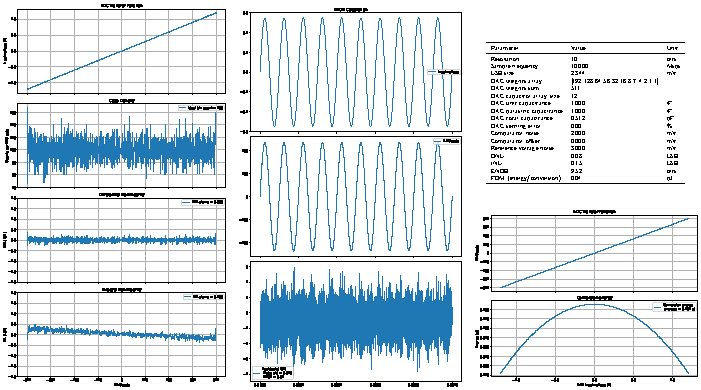
\includegraphics[width=\textwidth]{behavioral_10b_noisy_scadec_combine.pdf}}
% \frame{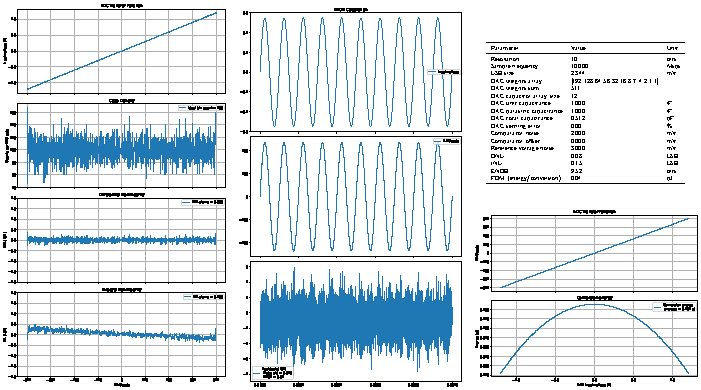
\includegraphics[width=\textwidth]{behavioral_10b_noisy_scadec_combine.pdf}}
% \frame{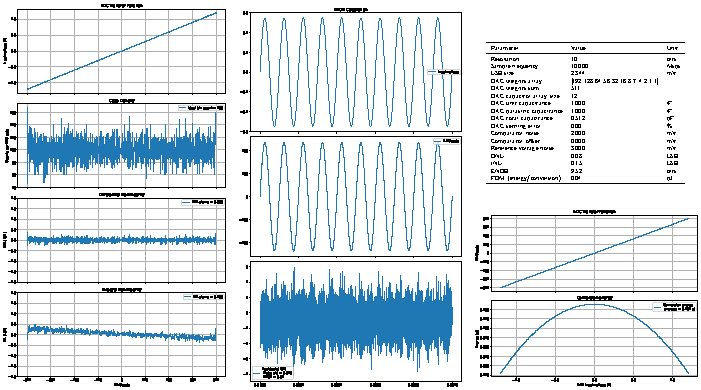
\includegraphics[width=\textwidth]{behavioral_10b_noisy_scadec_combine.pdf}}
% \frame{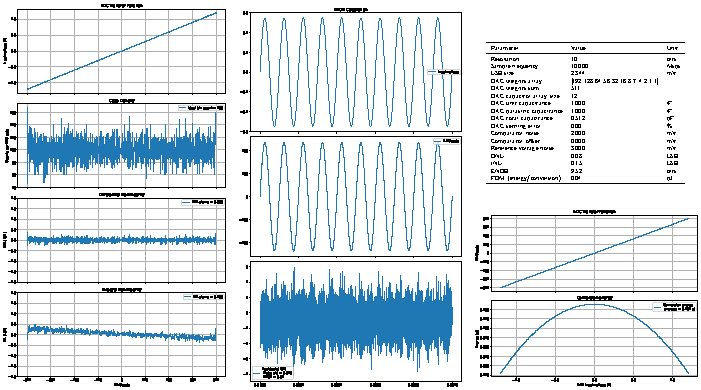
\includegraphics[width=\textwidth]{behavioral_10b_noisy_scadec_combine.pdf}}
% \frame{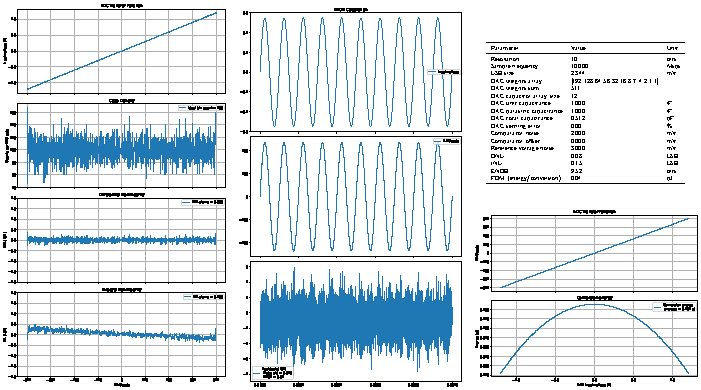
\includegraphics[width=\textwidth]{behavioral_10b_noisy_scadec_combine.pdf}}


\frame{\frametitle{10-bit w/ noise and postconversions}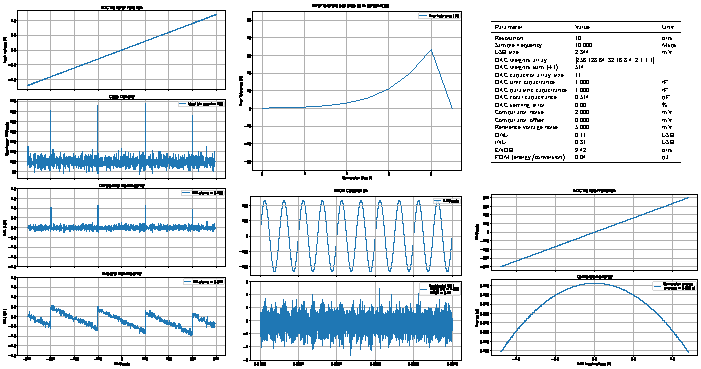
\includegraphics[width=\textwidth]{behavioral_10b_noisy_postconv_combine.pdf}}
\frame{\frametitle{10-bit w/ noise and split MSB}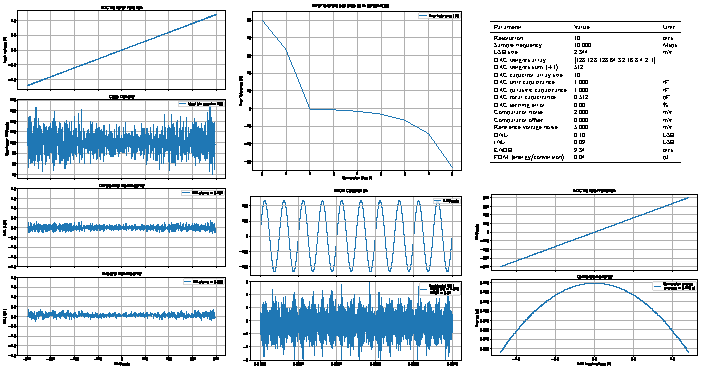
\includegraphics[width=\textwidth]{behavioral_10b_noisy_splitmsb_combine.pdf}}
\frame{\frametitle{10-bit w/ noise and radix 1.75}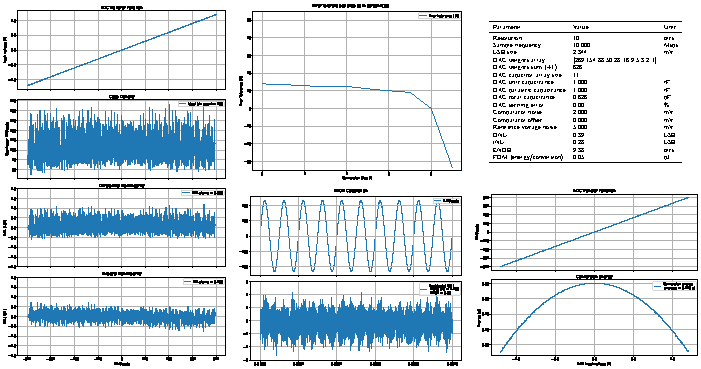
\includegraphics[width=\textwidth]{behavioral_10b_noisy_radix175_combine.pdf}}
\frame{\frametitle{10-bit w/ noise and radix 1.75 normalized}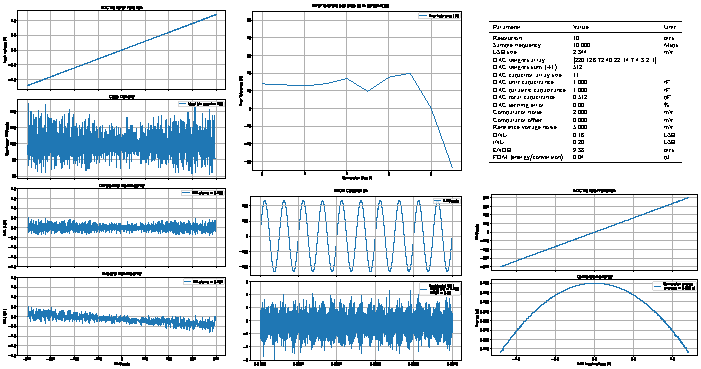
\includegraphics[width=\textwidth]{behavioral_10b_noisy_radix175norm_combine.pdf}}
\frame{\frametitle{10-bit w/ noise and binary compensation}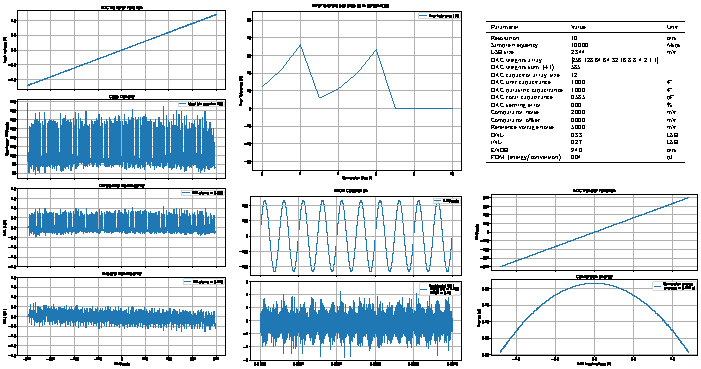
\includegraphics[width=\textwidth]{behavioral_10b_noisy_bincomp_combine.pdf}}
\frame{\frametitle{10-bit w/ noise and binary recombination}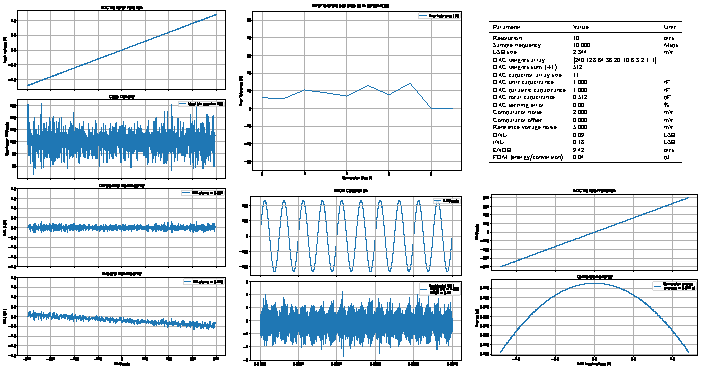
\includegraphics[width=\textwidth]{behavioral_10b_noisy_binrecomb_combine.pdf}}
\frame{\frametitle{10-bit w/ noise and SC-ADEC}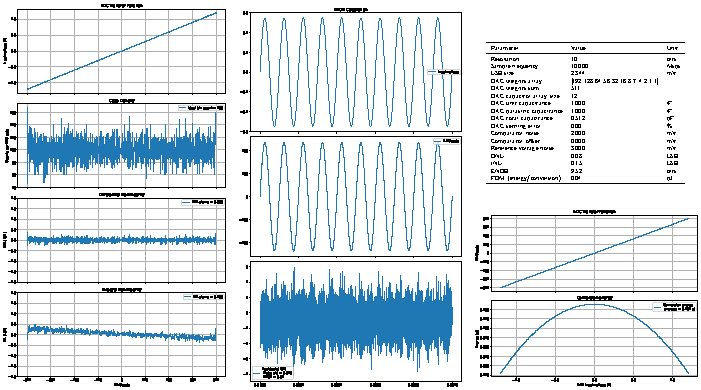
\includegraphics[width=\textwidth]{behavioral_10b_noisy_scadec_combine.pdf}}

\frame{\frametitle{10-bit w/ settling error}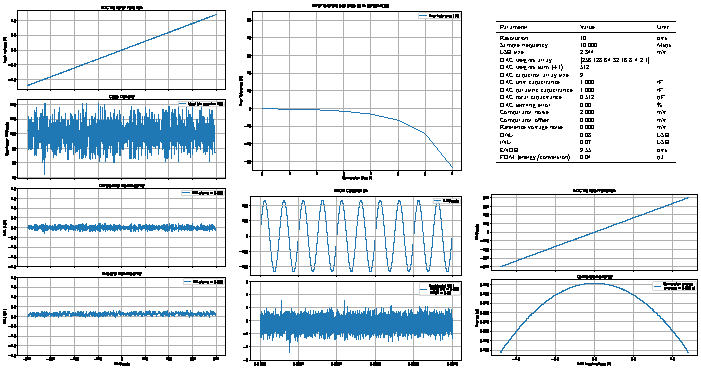
\includegraphics[width=\textwidth]{behavioral_10b_seterror_combine.pdf}}
\frame{\frametitle{10-bit w/ settling error and binary recombination}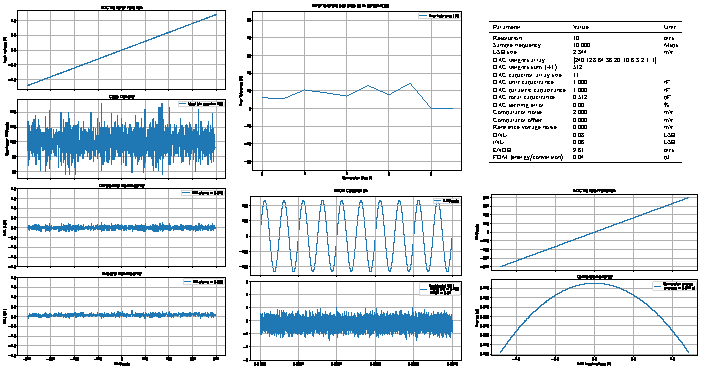
\includegraphics[width=\textwidth]{behavioral_10b_seterror_binrecomb_combine.pdf}}
\frame{\frametitle{10-bit w/ settling error and SC-ADEC}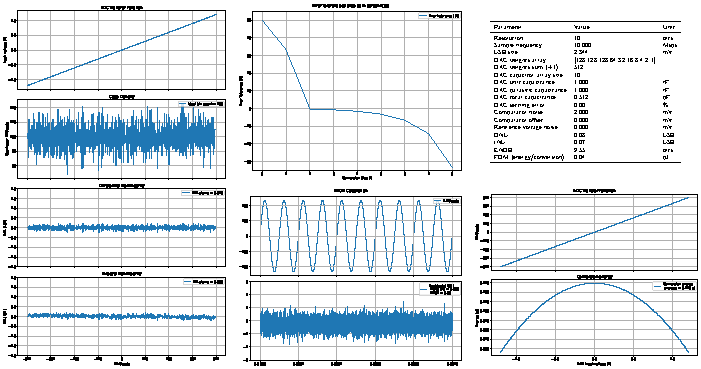
\includegraphics[width=\textwidth]{behavioral_10b_seterror_splitmsb_combine.pdf}}

\frame{\frametitle{10-bit w/ mismatch}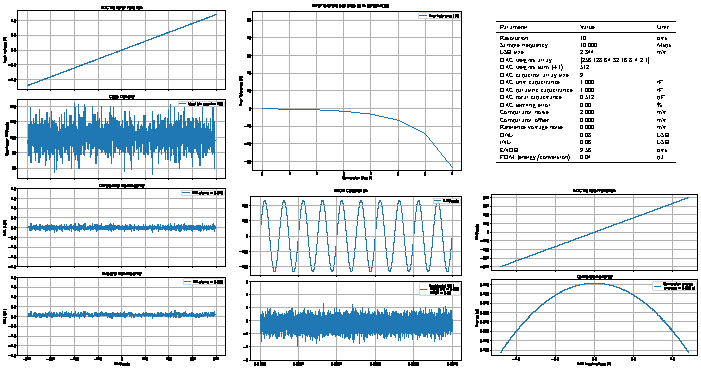
\includegraphics[width=\textwidth]{behavioral_10b_mismatch_combine.pdf}}
\frame{\frametitle{10-bit w/ mismatch and binary recombination}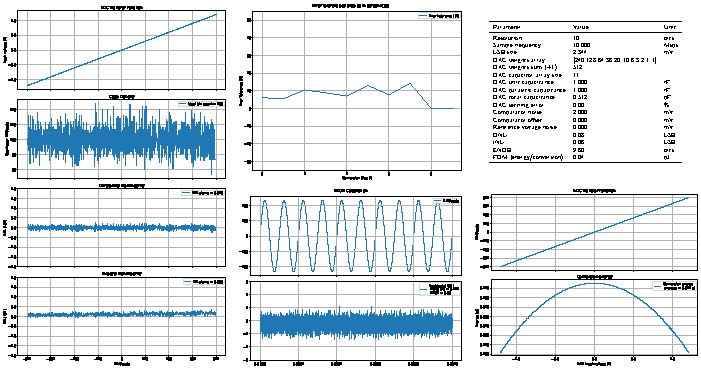
\includegraphics[width=\textwidth]{behavioral_10b_mismatch_binrecomb_combine.pdf}}
\frame{\frametitle{10-bit w/ mismatch and radix 1.75 normalized}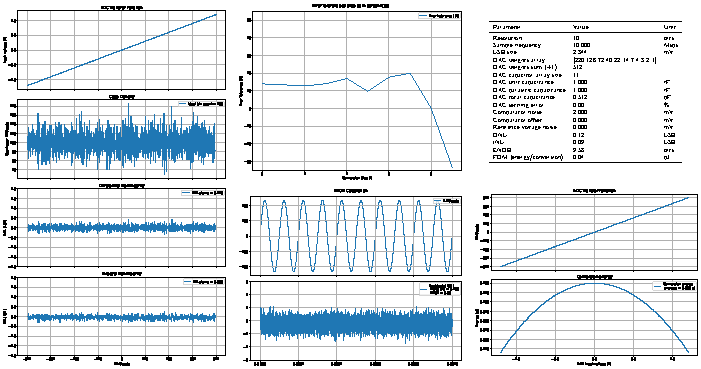
\includegraphics[width=\textwidth]{behavioral_10b_mismatch_radix175norm_combine.pdf}}
\end{document}